\documentclass[12pt]{book}
\usepackage[a4paper,left=1.5in, right=1.2in, top=1in, bottom=1in, includefoot, headheight=13.6pt]{geometry}
\usepackage[utf8]{inputenc}
\usepackage[T1]{fontenc}
\usepackage[a4paper]{geometry}
\usepackage{minted}
\usepackage{csquotes}
\usepackage[spanish,french,main=english]{babel}
\usepackage{fancyhdr}
\usepackage{titling}
\usepackage{epigraph}
\usepackage{graphicx}
\usepackage{tabularx}
\usepackage{makecell,siunitx}
\usepackage{multirow}
\usepackage{enumitem}
\usepackage{amssymb}
\usepackage{multicol}
\usepackage{placeins}
\usepackage{xspace}
\usepackage{subcaption}
\usepackage[table,xcdraw]{xcolor}
\usepackage[autolanguage]{numprint}
\usepackage[backend=biber,style=alphabetic]{biblatex}
\usepackage{lipsum}

\renewcommand*{\labelalphaothers}{}

\robustify\bfseries

% Links
\usepackage{hyperref}
\hypersetup{
    colorlinks=true,
    linkcolor=blue,
    filecolor=magenta,      
    urlcolor=cyan,
    citecolor=blue
}

% URL if DOI not present
\DeclareSourcemap{
  \maps[datatype=bibtex]{
    \map[overwrite]{
      \step[fieldsource=doi, final]
      \step[fieldset=url, null]
      \step[fieldset=eprint, null]
    }  
  }
}

%\usepackage[acronym,toc]{glossaries}
\usepackage[acronym]{glossaries-extra}
\setabbreviationstyle[acronym]{long-short}

\graphicspath{{images/}}

% Title, author
\title{Navigating Diverse Datasets in the Face of Uncertainty}
\author{Alejandro Álvarez Ayllón}
\date{\today}

% Page style
\pagestyle{fancy}
\setlength{\headheight}{28pt}
\fancyhead[LE,RO]{}
\fancyhead[RE,LO]{\rightmark}
\fancyfoot[CE,CO]{\thepage}

% Space between paragraphs
\parindent 0pt
\parskip 1.5ex

% extra spacing
\renewcommand{\baselinestretch}{1.33}

% Quotations
\renewcommand{\mkbegdispquote}[2]{\itshape}

% Et al
\newcommand{\etal}{\textit{et al}. }

% Math symbols
\newcommand{\eqdist}{\stackrel{d}{=}}

% Quotes in italic
\renewcommand{\mkbegdispquote}[2]{\itshape}

% Table header bold
\renewcommand\theadfont{\bfseries}% bold tabular headers

% Align on +/-
\sisetup{separate-uncertainty}

% Epigraph style
\setlength\epigraphrule{0pt}
\setlength\epigraphwidth{.6\textwidth}

% Environments
\newtheorem{example}{Example}
\newtheorem{definition}{Definition}
\newtheorem{property}{Property}
\newtheorem{proof}{Proof}

% Bibliography
\addbibresource{references.bib}

% Glossary
\makeglossaries

\newacronym{Cosmos}{Cosmos}{Cosmic Evolution Survey}
\newacronym{CDF}{CDF}{Cumulative Distribution Function}
\newacronym{CERN}{CERN}{European Organization for Nuclear Research}
\newacronym{CRISPDM}{CRISP-DM}{CRoss Industry Standard Process for Data Mining}
\newacronym{CSV}{CSV}{Comma-separated Values}
\newacronym{ECDF}{ECDF}{Empirical Cumulative Distribution Function}
\newacronym{EMD}{EMD}{Earth-Mover Distance}
\newacronym{FK}{FK}{Foreign-Key}
\newacronym[longplural=Equally-Distributed Dependencies]{EDD}{EDD}{Equally-Distributed Dependency}
\newacronym[longplural=Unary Equally-Distributed Dependencies]{uEDD}{uEDD}{Unary Equally-Distributed Dependency}
\newacronym{FITS}{FITS}{Flexible Image Transport System}
\newacronym{FWHM}{FWHM}{Full Width at Half Maximum}
\newacronym{HEP}{HEP}{High Energy Physics}
\newacronym{IDE}{IDE}{Interactive Data Exploration}
\newacronym{KLD}{KL Divergence}{Kullback-Leibler Divergence}
\newacronym[longplural=Inclusion Dependencies]{IND}{IND}{Inclusion Dependency}
\newacronym{JCR}{JCR}{Journal Citation Reports}
\newacronym{KDD}{KDD}{Knowledge Discovery in Databases}
\newacronym{KiDS}{KiDS}{Kilo Degree Survey}
\newacronym{PDF}{PDF}{Probability Density Function}
\newacronym{PK}{PK}{Primary-Key}
\newacronym{PGN}{PGN}{Probabilistic Graphical Network}
\newacronym{Q1}{Q1}{First quartile}
\newacronym{SDSS}{SDSS}{Sloan Digital Sky Survey}
\newacronym{SOM}{SOM}{Self-Organizing Map}
\newacronym{ESOM}{ESOM}{Emergent Self-Organizing Maps}
\newacronym{SVM}{SVM}{Support Vector Machine}

% Used: \gls{SDSS}

% Aliases for Find2, Mind and PresQ to avoid repeating textsc
\newcommand{\Find}[0]{\textsc{Find2}\xspace}
\newcommand{\Mind}[0]{\textsc{Mind}\xspace}
\newcommand{\Zigzag}[0]{\textsc{Zigzag}\xspace}
\newcommand{\PresQ}[0]{\textsc{PresQ}\xspace}
\newcommand{\PresQG}[0]{\textsc{PresQ(G)}\xspace}
\newcommand{\Hyperclique}[0]{\textsc{Hyperclique}\xspace}
\newcommand{\SOMA}[0]{\textsc{SOMA}\xspace}

% Code environment
\newenvironment{code}{\captionsetup{type=listing}}{}
\renewcommand\listingscaption{Code}

\usemintedstyle{vs}
\setminted{
frame=lines,
bgcolor=lightgray,
linenos,
framesep=2mm,
baselinestretch=1.2,
fontsize=\footnotesize
}

% Document
\begin{document}

\frontmatter

\begin{titlepage}
\begin{center}
    \vspace*{1cm}
    
    \Huge
    \textbf{\thetitle}
    
    %\vspace{0.5cm}
    % Subtitle
    
    \vspace{1.5cm}
    
    \Large
    \textbf{\theauthor}
    
    \vfill
    
    A thesis presented for the degree of \\
    Doctor in Computer Engineering
    
    \vspace{0.8cm}
    
\includegraphics[width=0.3\textwidth]{images/uca-logo.pdf}
    
    \vspace{0.5cm}
    
    \large
    Departamento de Ingeniería Informática \\
    Universidad de Cádiz \\
    España \\
    \today
    
\end{center}
\end{titlepage}

\chapter*{Resumen}
\begin{otherlanguage}{spanish}
\lipsum[1-2]
\end{otherlanguage}

\chapter*{Abstract}
\lipsum[1-2]

\chapter*{Agradecimientos}
\begin{otherlanguage}{spanish}
\lipsum[10-11]
\end{otherlanguage}

% Style reference
\chapter*{Style reference}
In this document the following style guide is used:

\begin{displayquote}
    Literal quotations from other authors are indented, and in italics.
\end{displayquote}

The name of algorithms and software products are written with \textsc{Small Caps};
names of variables, filenames, etc. are displayed with a \texttt{fixed-width font}.

\begin{listing}[ht]
\begin{minted}{python}
def code_is_inlined():
    """
    With a fixed-width font and syntax highlighting whenever possible
    """
    pass
\end{minted}
\caption{Code example}
\end{listing}


% Table of content, figures, etc.
\cleardoublepage
\tableofcontents

\cleardoublepage
\addcontentsline{toc}{chapter}{\listfigurename}
\listoffigures

\cleardoublepage
\addcontentsline{toc}{chapter}{\listtablename}
\listoftables

\cleardoublepage
\renewcommand\listoflistingscaption{List of Codes}
\addcontentsline{toc}{chapter}{\listoflistingscaption}
\listoflistings

\printglossary
\printglossary[type=\acronymtype,title=List of Acronyms, toctitle=List of Acronyms]
\glsresetall

% Epigraph
\chapter*{}
\markboth{}{}
\epigraph{
\foreignlanguage{french}{\textit{Il semble que la perfection soit
atteinte non quand il n'y a plus rien à ajouter, mais quand il n'y
a plus rien à retrancher.}}
}{--- Antoine de Saint Exupéry}

\mainmatter

\chapter{Introduction}
\label{chapter:introduction}

Nowadays, it is not uncommon for many types of users
--- from proficient data scientists to enthusiasts without formal
training, from finance to physics --- to dive into overwhelming
data sets looking for any relevant pattern they can find. This data
may consist of files that have not yet been ingested into a
database system. The researcher must curate
these files, understand and sieve their content, and 
extract and communicate information. This activity
is known as \emph{data exploration}, and it is an integral part
of a new, data-intensive process of doing science that
can be considered a new paradigm of scientific exploration,
the fourth after the experimental, theoretical, and computer-simulation paradigms~\cite{bell2009beyond,hey2009the}.

Data exploration is also known as \gls{KDD}
because ``knowledge'' is the product of this process
\parencite{Piatetsky-Shapiro1991,Fayyad1996a}.
\emph{Data Mining} is sometimes used as a synonym or as an integral
part, as shown in figure~\ref{fig:kdd} \cite{Fayyad1996a,Reinartz1999}.
The latter interpretation is preferred for this work. 

\begin{figure}[htbp]
    \centering
    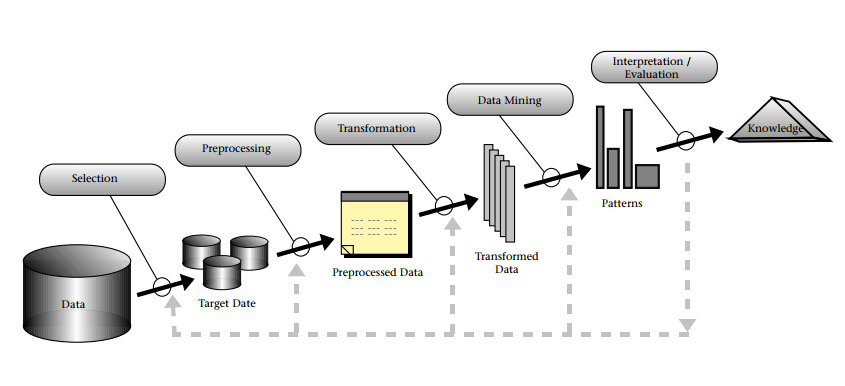
\includegraphics[width=\linewidth]{images/1_introduction/kdd.jpg}
    \caption{\glsfmtfull{KDD}.}
    \label{fig:kdd}
\end{figure}

The \gls{CRISPDM}~\cite{Shearer2000} proposes a model for the data
mining step, composed of six phases, shown in figure~\ref{fig:crispdm}:

\begin{description}
    \item[Business Understanding] Definition of the requirements and objectives of a data mining project
        from the business (or domain) perspective.
    \item[Data Understanding] Familiarization with the data collection. Domain knowledge
        is needed to understand the data, but the original project can be refined as the data is best understood.
    \item[Data Preparation] Attribute selection, cleaning, imputation, \ldots are applied over the raw data.
    \item[Modeling] Various modeling techniques are implemented, calibrated and assessed. Different models may require different data preparation ---
    for instance, cleaning, imputation, or normalization.
    \item[Evaluation] The proposed models need to be thoroughly reviewed to make sure they meet the required quality and that they achieve the stated
    objectives.
    \item[Deployment] The new knowledge has to be useful and actionable.
    Depending on the original objectives, the model can be integrated 
    or transformed into an automatic system; or ``simply'' summarized into a report.
\end{description}

\begin{figure}[htb]
    \centering
    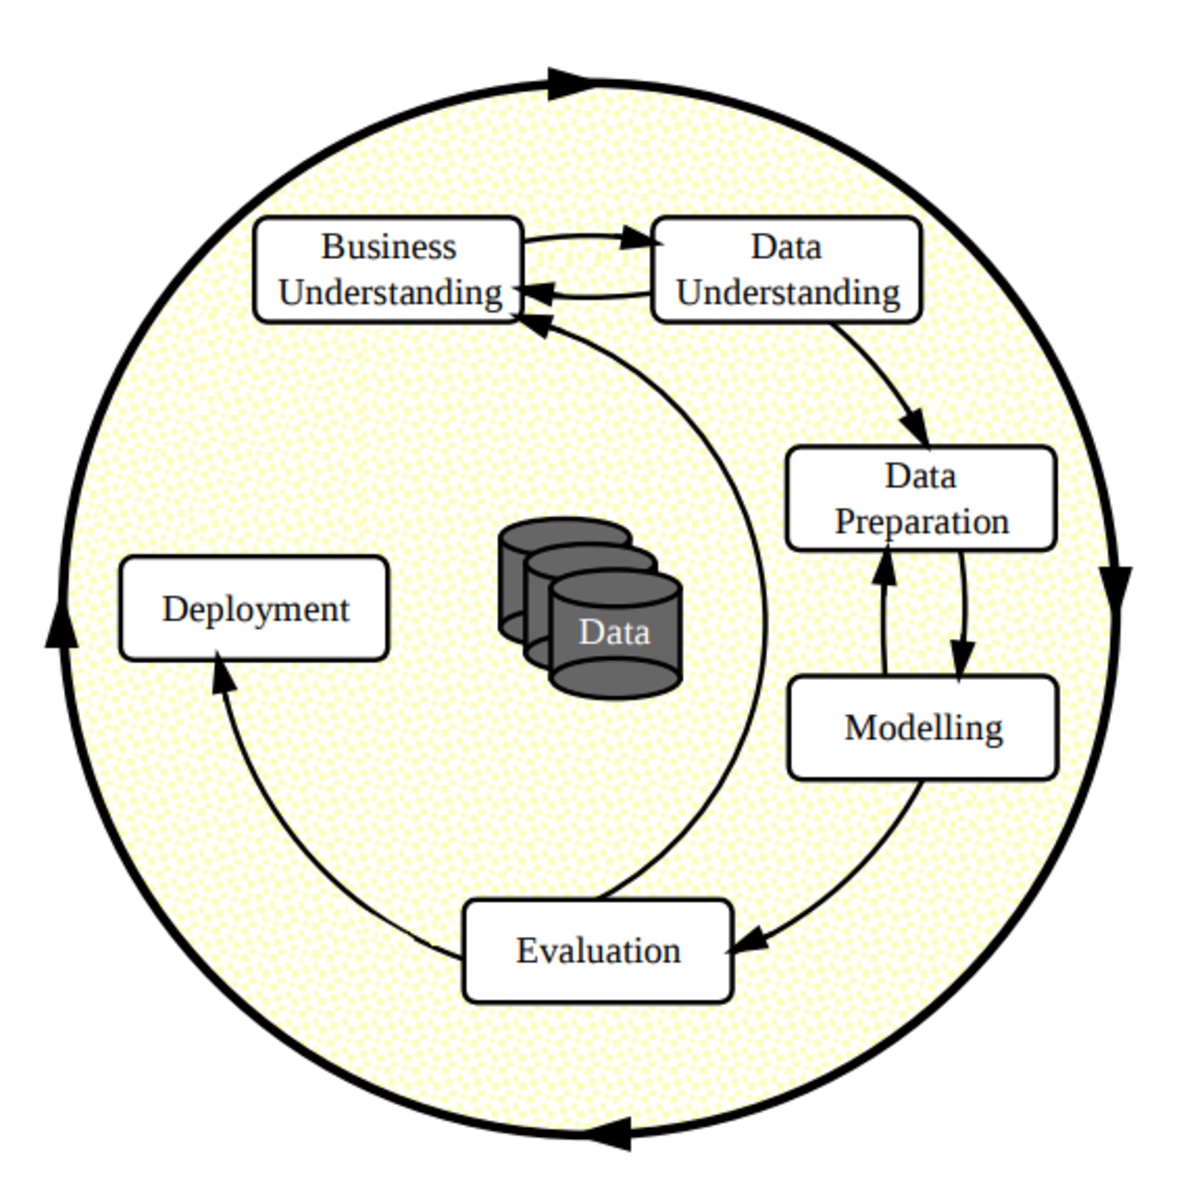
\includegraphics[width=0.8\linewidth]{images/1_introduction/crisp-dm.pdf}
    \caption{\glsfmtfull{CRISPDM}.}
    \label{fig:crispdm}
\end{figure}

In this thesis, we focus on the \textbf{Data Understanding} phase, where the user interactively
explores the data, gaining insight, and generating hypotheses during the process.

When starting the initial analysis, the data may be in a \emph{raw} format: unprocessed files not 
optimized for access. Even worse, their schema may be inconsistent or poorly documented, and they may
originate from different sources. These factors combined make the task of the data scientist more
difficult:

\begin{itemize}
    \item Ingestion into a ``proper'' database introduces latency. Since the data is not well
        understood, any early design decision will soon become obsolete~\cite{Kersten2011}.
        Techniques for \emph{in-situ} exploration try to overcome this difficulty
        by allowing direct examination of the data files performantly~\cite{Idreos2011}.
    \item The data may be split into multiple files~\cite{Baud2012}, and these files may not
        follow the same schema~\cite{Alawini2014}. Data profiling and schema-matching tools
        can be helpful for this type of problem.
\end{itemize}

Astronomy is an example of a scientific discipline where there are vast amount of digitized data
readily accessible to the scientist, and, therefore, where \emph{Data Mining} has been gaining
more momentum~\cite{Ball2010}. A considerable portion of this data is made available by the community
itself as independent files with little to no coordination in terms of schema consistency~\cite{Pepe2014}.
Unfortunately, existing \emph{in-situ} techniques leave out schema-matching, while the existing
data profiling approaches require either relational data from discrete domains or they are restricted to matching based on a single attribute. This motivates our
research.

\section{Objectives}
\label{sec:main_objective}

Given the problem stated above, the main objective of this
thesis is:

\begin{quote}
    To assist data scientists during the exploration of 
    unprocessed, numerical, raw data distributed across
    multiple files based solely on its intrinsic distribution.
\end{quote}

To make this objective attainable, we define the following sub-objectives:

\begin{enumerate}
    \item \textbf{Find existing techniques} that help users
        to  explore the data \emph{in-situ}. A survey of the 
        literature help users by directing them to algorithms
        and tools suitable for their use case.
        
    \item \textbf{Identify gaps in the coverage of the existing
        techniques}, helping to direct the effort of present
        and future research into areas that need better
        coverage, widening the options available to users.

    \item \textbf{Design new algorithms} tailored to numerical 
    and uncertain data that cover part of the identified gaps,
    putting new tools at the disposal of data scientists.
\end{enumerate}
\label{enum:objectives}

\section{Structure of this document}

First, we described the methodology followed for this thesis in chapter~\ref{chapter:methodology}.
Chapter~\ref{chapter:literature_review} contains a systematic literature mapping
of the \emph{in-situ} processing of scientific data.
Then, chapter~\ref{chapter:diverse} identifies gaps in the literature regarding
the exploration of diverse numerical datasets and summarizes some initial prototypes
that remain open for further research.
Chapter~\ref{chapter:presq} proposes an algorithm suitable for schema matching
tailored to scientific data. Chapter~\ref{chapter:som} outlines a statistical
test based on \glspl{SOM}, which can bridge the gap between schema matching and
\emph{in-situ} access.
Chapter~\ref{chapter:discussion} discusses our contributions
and analyses the threats to the validity of the present thesis.
Finally, chapter~\ref{chapter:conclusions} summarizes our findings and contributions and proposes potential future lines of work.


\chapter{Methodology}
\label{chapter:methodology}
We use \emph{Researching Information Systems and Computing}~\cite{Oates2006} as the
general framework for defining the methodology for our research. On it, Oates describes
six fundamental aspects of research, using the mnemonic `6P':

%\begin{itemize}
    %\item \textbf{Purpose}: The reason for doing the research.
    %\item \textbf{Products}: Its outcomes.
    %\item \textbf{Process}: The sequence of activities.
    %\item \textbf{Participants}: People involved with the research.
    %\item \textbf{Paradigm}: Way of thinking.
    %\item \textbf{Presentation}: Dissemination and explanation of the research.
%\end{itemize}

\paragraph{Purpose}
\label{method:purpose}
A research project needs a well-defined objective in order to be able
to define what means for it to succeed --- either totally or partially.

To be honest, the final objective of this project is \emph{obtaining the
degree of Doctor in Computer Engineering}. This is important to define
a hierarchy of objectives, from the most general to the most specific. 

With this objective in mind, the current research project must
\emph{increase the body of knowledge} of its area. Had we not been honest
about the final objective, we could have risked a purely technical approach.

Nevertheless, we want to \emph{solve an existing problem}. In our case,
as discussed on chapter~\ref{chapter:introduction}, we target the
\gls{IDE} research area.

\paragraph{Products}
\label{method:products}
Oates lists five different types of contributions to the body of knowledge, based on
an existing classification from Davis \& Parker\cite{Oates2006,Davis1997}:
evidence, methodology, analysis, theories, and computer-based products. Note
that an improvement of an existing product is still considered a contribution.

For the current thesis, we aim to produce a new computer-based product
for \gls{IDE}, understanding as such novel algorithms and techniques.
The literature review is also a contribution (analysis).

\paragraph{Process}
\label{method:process}

\begin{figure}[htpb]
  \centering
  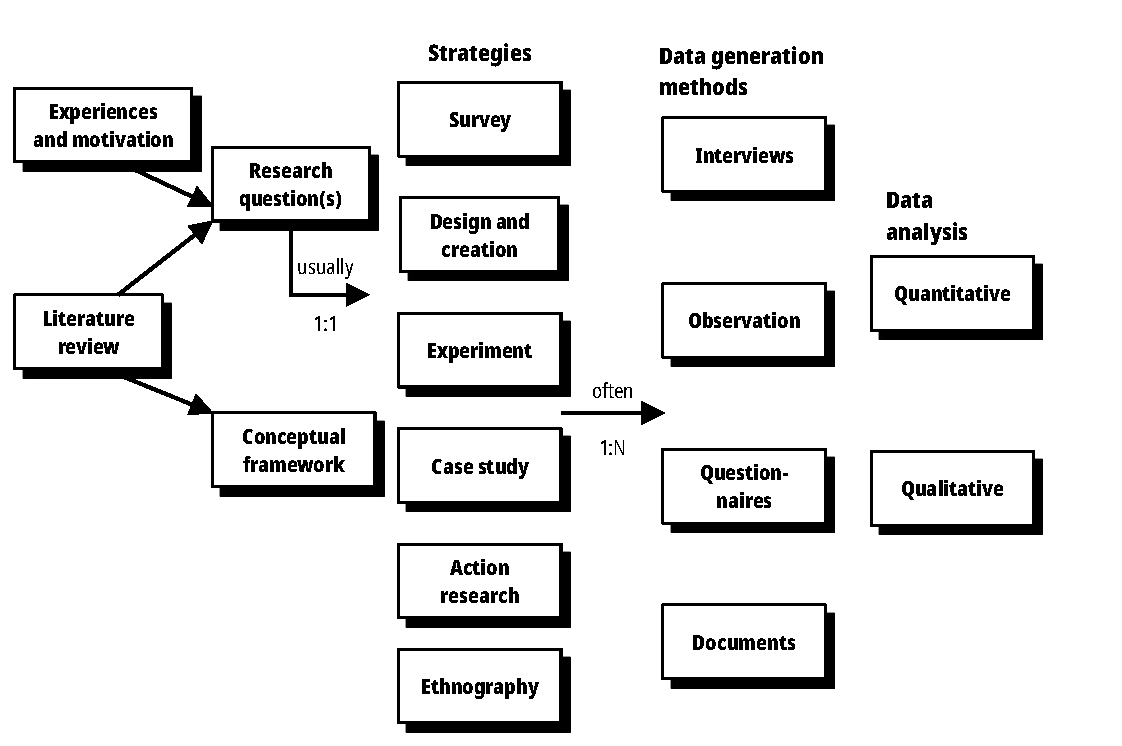
\includegraphics[width=\linewidth]{images/2_methodology/modelo_proceso}
  \caption[Model of the research process]{Model of the research process~\cite{Oates2006}}
  \label{fig:method_process_model}
\end{figure}

Figure~\ref{fig:method_process_model} shows the model of the research process.
The time working at \gls{CERN} and at the \emph{Astronomy Department of the University of Geneva}
set up the experiences and motivations for this research: \gls{IDE} on physical measurements,
which have an intrinsic uncertainty. In chapter~\ref{chapter:introduction} we have
introduced the research questions for this thesis.
We will be shortly defining the methodology for the literature review,
the research strategy, the data generation methods, and data analysis.

\paragraph{Participants}
\label{method:participants}
The direct participants of the current research will be the researcher, the tutor, and
the thesis director. Journal editors and reviewers are indirect participants.

\paragraph{Paradigm}
\label{method:paradigm}
The paradigm is the philosophical model that frames the research.
It defines what the researcher believes\footnotemark on the nature
of reality (\emph{ontology}), how the researcher interacts with
knowledge (\emph{epistemology}), and how knowledge is acquired
(\emph{methodology})~\cite{Guba1990}.
\footnotetext{By definition, this framework can not be proven~\cite{Guba1994}.}

We can find different classifications of different paradigms depending on
their views on these questions. For instance, Oates and Chua~\cite{Chua1986}
consider three branches: `positivism' (reality is objective and the researcher neutral),
`interpretative' (truth is subjective and subject to the context), and
`critic research' (the social structure is the main focus).
Shull \etal~\cite{Shull2008} extends this classification with a fourth paradigm:
the \emph{pragmatism}. In this paradigm, knowledge is evaluated based on its
utility and is considered, in any case, approximate.

Considering our purpose and objective, and given the restricted list of
participants, we will follow the paradigm of \emph{pragmatism} for this research project.

\paragraph{Presentation}
\label{method:presentation}
The main results from our research are compiled into the present thesis
and published in peer-reviewed journals. Drafts have been published in \texttt{arXiv}.
All the relevant source code is publicly available.

\section{Literature review}
\label{sec:method_literature_review}
A systematic mapping study is a process for the exploration of the
situation of a wide research area with a high level of granularity,
allowing us to identify areas in the domain where it may be interesting to
explore in more detail~\cite{Kitchenham2007}. Because we are trying to obtain
an overview of the situation of the research on data exploration techniques
and identify where additional work may be required, we have decided to follow this
approach, and, more specifically, the guidelines proposed in
\emph{Systematic Mapping Studies in Software Engineering}~\cite{Petersen2007}.
For completeness, we include in figure \ref{fig:systematicmapping_diagram} the
diagram of the process for a systematic mapping study, as defined by
Petersen \etal.

\begin{figure}[htbp]
    \centering
    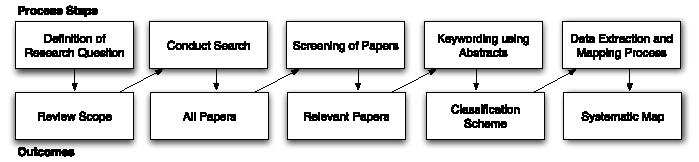
\includegraphics{images/3_mapping/systematicmapping_diagram}
    \caption{The Systematic Mapping process}
    \label{fig:systematicmapping_diagram}
\end{figure}

\section{Research strategy}
\label{sec:method_strategy}
From the list of strategies shown in figure~\ref{fig:method_process_model},
we follow \emph{Design and Creation} and \emph{Experiments}.

\paragraph{Design and Creation} Is an adequate strategy since we aim for a
computer-based product. The resulting artifacts should be carefully studied
and developed and result from a careful engineering approach.
Thus, we follow \emph{Engineering Design}:
    
\begin{displayquote}
  Engineering design is the systematic, intelligent generation and evaluation
  of specifications for artifacts whose form and function achieve stated
  objectives and satisfy specified constraints~\cite{Dym2012}.
\end{displayquote}

Figure~\ref{fig:engineering_design} summarizes the different stages for this method.
We want to emphasize that this method is inherently iterative since each stage
provides feedback to the precedent stages. This work results from many such
iterations: the research plan defined the initial task: \gls{IDE} of raw scientific data.
We performed a systematic literature mapping to identify solution principles and existing problems.
As a result of this literature review, we refined the initial task: data exploration of multiple files with related raw scientific data but incomplete metadata.

\begin{figure}[htbp]
  \centering
  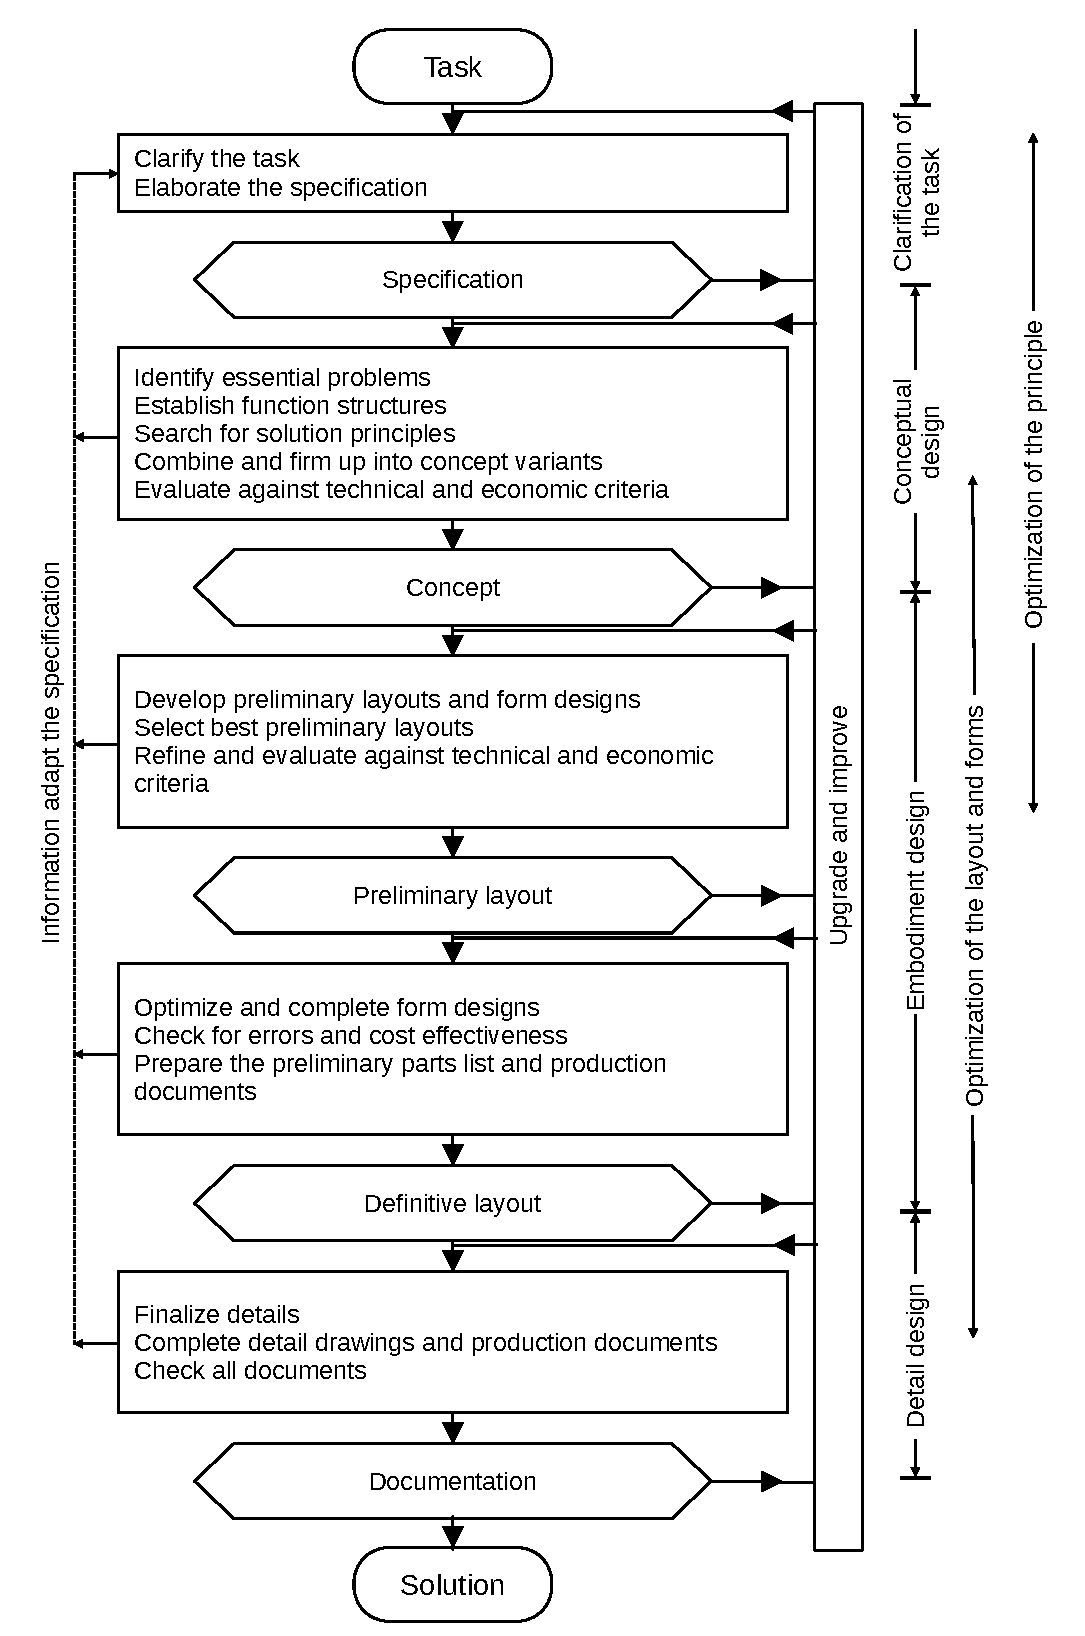
\includegraphics[width=\linewidth]{images/2_methodology/design_process}
  \caption[Engineering Design]{Engineering Design~\cite{Dym2012,Pahl1984}}
  \label{fig:engineering_design}
\end{figure}

\paragraph{Experiments} \emph{Engineering Design} incorporates the development of
multiple preliminary products, which need to be compared and evaluated before refining
them into the final deliverable. Thus, experiments are a central aspect of this method.

%Research question introduction (chap.1), literature review chap.3 (link with methodology here).
%Data generation, observations (experiments), Data Analysis quantitative and qualitative (SOM),
%link with chapter about discussion/results?
%Documentation is the thesis itself.
%Insist on the feedback loop!

%Task -> Specification -> Concept -> Preliminary chap 4 (bridge, plus preliminary excuse for dead ends)
%Definitive layout 5 and 6 (presq and som).


\section{Data generation methods}
From the proposed data generation methods, we use \textbf{documents},
such as scientific papers to obtain datasets for the experiments.

With these datasets, we run experiments and \textbf{observe} the results,
using performance metrics to compare different algorithms and their parameterizations.

\section{Data analysis}
We base our comparisons on \textbf{quantitative} metrics: run-time, success rate,
statistical significance, etc.

\section{Open Science}
This research adheres to the \emph{Open Science} principles~\cite{oro44719}.

\begin{itemize}
    \item \textbf{Open Access} Papers are published either on \emph{Open Access} journals,
        or made accessible on pre-print servers.
    \item \textbf{Open Data} The results from our experiments are uploaded to a public
        server (such as \textsc{GitHub}, together with the source code, using \texttt{git-lfs}).
    \item \textbf{Open Reproducible Research} 
        \begin{itemize}
            \item \textbf{Open Notebooks} Notebooks used to summarize the results are
                included next to the source code.
            \item \textbf{Open Source} The source code is under a permissive free software license
                (MIT\footnote{\url{https://opensource.org/licenses/MIT}}).
            \item \textbf{Reproducibility Guidelines} Even if the original results become
            inaccessible, the repositories include a list of the required dependencies so the
            environment can be replicated. The procedure followed to generate our results is documented.
        \end{itemize}
    \item \textbf{Open Repositories} All the delivered software is in \textsc{GitHub},
        and a copy archived in \href{https://zenodo.org/}{\textsc{Zenodo}}~\cite{zenodo} with an
        associated DOI. Papers are available in pre-print servers such as
        \href{https://arxiv.org/}{\textsc{arXiv}} and
        \href{https://www.techrxiv.org}{\textsc{TechRxiv}}.
\end{itemize}


\chapter{Literature Review}
\label{chapter:literature_review}
\glsresetall

Following the \emph{Engineering Design Process}, we have defined the task in
section~\ref{enum:objectives}. For clarification, and as a required step prior
to identifying the essential problems and solution principles, the natural next
step is a literature review, one of the initial stages of our process.

This chapter summarizes the results of the \emph{Systematic Mapping of the Literature},
following the method defined in section~\ref{sec:method_literature_review}.

Since the \emph{Engineering Design Process} is iterative and includes feedback loops, in
section~\ref{sec:mapping/overview}, we estate the objectives of the
\emph{original} literature mapping. These objectives were later refined,
incorporating the results of this study.
In section~\ref{sec:mapping/method}, we describe our method.
In section~\ref{sec:mapping/results}, we summarize the results of the literature mapping.
Finally, in section~\ref{sec:mapping/discussion}, we discuss the interpretation of our findings
and insights.

Part of the content of this chapter appears in the article \emph{Interactive Data Exploration
of Distributed Raw Files: A Systematic Mapping Study}~\cite{Alvarez2019},
published on IEEE Access.

\section{Overview}
\label{sec:mapping/overview}
\gls{IDE} tools target the Data Understanding phase of \gls{CRISPDM}. They have
human intuition as a core part of the process, where the user tentatively
explores the data, iterating and reformulating the queries as
their knowledge and insight changes with each iteration.

A system that is able to be used in such a way needs to be lightweight, adaptive
and have reasonably low response times---\cite{Miller1968} considers two seconds
to be the upper limit for the continuity of thoughts---,
helping and assisting, without getting in the way of the person involved in
the loop.

Because of this exploratory nature, any early decision on data structure,
storage and indexing are inappropriate~\cite{Kersten2011}. They introduce latency,
and optimize for a pattern that only happens for a brief period of time.

This problem can be tackled at different levels---from the physical layout on disk,
to the interface interacting with the user. In 2015, Idreos~\cite{Idreos2015}
classified several of these solutions depending on which approach they take
on the issue. This paper originally attracted our attention  due to the potential
applications in \gls{HEP}\footnotemark, although
the techniques found can be of interest for other scientific domains.

\footnotetext{
    This research was initiated while employed at \gls{CERN},
    so \gls{HEP} was the original target use case
}

In summary, we need to satisfy three main requirements:

\begin{enumerate}
  \item \emph{Interactive response times}, as already discussed
  \item \emph{Access to raw data files}. Pre-loading data in main memory is not an
    option due to the data volume and because we aim for a system that extends and does
    not replace the existing data management solution
  \item Ideally, \emph{distributed}, since files are stored and replicated by an already existing
    distributed storage system~\cite{Baud2012}.
\end{enumerate}

The granularity of the access has to be higher than \emph{file level} because
scientists normally care about datasets that are defined by the data origin,
year, conditions, etc\ldots, and one dataset may be distributed across
several files.

\section{Method}
\label{sec:mapping/method}

Idreos \etal~\cite{Idreos2015} propose a classification of different possible approaches
to our problem.
This study provides an excellent introduction but we wanted to expand on it by answering
two questions that were not covered by the original paper and we also wished to survey
the subsequent evolution of the domain.

\subsection{Research questions}
\label{sec:mapping/research_questions}

\subsubsection{RQ1. How has the research area evolved?}
Given that this is an active research area, it has probably progressed since
the tutorial that we are using as a baseline. Therefore, the first
question to answer to decide how to focus future research is:
How has it evolved since 2015?

\subsubsection{RQ2. What is the maturity level of the research area?}
How many complete and reliable solutions are available?
Are they successfully implemented in practice?
How do they improve the users' experience? Identifying publications is not enough,
we also want to assess in what part of the software life-cycle they focus.

\subsubsection{RQ3. How far are we from a tool that solves our three requirements?}
The final target of this research is to identify solutions that cover our three
requirements.
Even though Idreos closed their tutorial by
mentioning the importance of interconnection research~\cite{Idreos2015}, they do not provide
any references or study on this area.

\subsection{Search strategy}
\label{sec:mapping/search_strategy}

For the retrieval of studies, it is necessary to clearly define
how the search is going to be performed. This work combines
three different strategies, as follows:

\begin{itemize}
  \item Set of known works obtained from \cite{Idreos2015} because our RQ2 is
    not covered by the original classification.
  \item Forward snowballing~\cite{Webster2002} from the known set of publications using Google Scholar.
  \item For completeness, database searches to improve the coverage of our study.
\end{itemize}

Jalali and Wohlin~\cite{Jalali2012} argue that snowballing and database searches
can lead to similar patterns but they also agree that it is
``not easy to draw any general conclusions'' about if the conclusions obtained are the same
using the two different approaches. Thus, we have opted to follow both.

The set of digital libraries consulted is:

\begin{itemize}
  \item ACM Digital Library
  \item Elsevier (Science Direct)
  \item Springer
  \item IEEE Digital Library
  \item Wiley Online Library
  \item World Scientific Net
\end{itemize}

Given the fast pace at which the field moves, older papers have been probably
superseded or, if still relevant, we expect them to be already included in \cite{Idreos2015}.
Consequently, we have limited the scope in time to studies published from 2010 onwards.

All of the references obtained by any of the previous method were imported into
a group in the \emph{Mendeley Reference Manager}. Any obviously non-interesting entry
---such as book or proceeding indexes---were removed at this stage.
The definitive list can be found on a public group in
\href{https://www.mendeley.com/community/interactive-data-exploration-in-science-systematic-mapping/}{Mendeley.com} and in
\href{https://www.zotero.org/groups/4517638/interactive-data-exploration-in-science-systematic-mapping/library}{Zotero.com}\footnotemark.

\footnotetext{Both groups are
    \texttt{interactive-data-exploration-in-science-systematic-mapping}
}

\subsection{Study selection criteria}
We based the initial screening of studies on title, abstract, and keywords.
In some cases, when the information provided by these fields was
insufficient to take a decision, we also considered their conclusions
or read the complete study.

We have focused here on finding primary studies related to data exploration.
The filtering was performed using the following exclusion criteria:

\begin{itemize}
  \item \emph{Unsupported language} Studies written in a language different than
  English, Spanish or French
  \item \emph{Incomplete publication} Abstract only, or presentations were excluded
  \item \emph{Off topic} Out of the data exploration domain
  \item \emph{Not a primary study} Secondary, tertiary and surveys
  \item \emph{Duplication} In case of duplication or high similarity for the same
  set of authors, only the most complete or the most recent was
  taken into account.
\end{itemize}

Those publications that passed the inclusion criteria were reviewed to make
sure all their fields were correct. Normally, this should have been done during
the previous stage but due to the sheer volume of publications yielded by the
search strategy this step was postponed until the filtering was done. Because only
title and abstract were used for the filtering, this did not affect the end
result.

\subsection{Classification}
Publications that pass the selection criteria will be classified into two axes:
data exploration facet and research type.

\subsubsection{Category}
\label{sec:mapping_category}
As mentioned in section~\ref{sec:mapping/research_questions}, we base our study on
the classification done by Idreos \etal~\cite{Idreos2015}, which is included for
convenience in table~\ref{tab:mapping/clustering}. For more details, we refer the
interested reader to Idreos' tutorial.

For our purposes, we have assigned one single category to each work covered
by our study, choosing the most prominent topic when more than one category
could fit.

\begin{table}[hptb]
  \footnotesize
  \begin{tabularx}{\textwidth}{>{\hsize=10.5em}X X X X}
    \hline
    \multicolumn{4}{l}{\textbf{User Interaction}} \\
    \hline
    \textit{Data Visualization} & Visual Optimizations & Visual Tools & \\
    \textit{Exploration Interfaces} & Automatic Exploration & Assisted Query Formulation & Novel Query Interfaces \\
    \hline
    \multicolumn{4}{l}{\textbf{Middleware}} \\
    \hline
    \textit{Interactive Performance Optimizations} & Data Prefetching & Query Approximation & \\
    \hline
    \multicolumn{4}{l}{\textbf{Database Layer}} \\
    \hline
    \textit{Indexes} & Adaptive Indexing & Time Series & Flexible Engines \\
    \textit{Data Storage} & Adaptive Loading & Adaptive Storage & Sampling \\
  \end{tabularx}
  \caption{Categories of Interactive Data Exploration solutions}\label{tab:mapping/clustering}
\end{table}

\subsubsection{Research type}
To answer our second research question---the maturity of the area---we follow
the classification of research approaches done by \cite{Wieringa2006},
as our guidelines for systematic mapping do~\cite{Petersen2007}.

We summarize the different research types in table~\ref{tab:mapping/research_type}.

As per this classification, we expect mature solutions that have been
implemented in practice to be covered by one or more \emph{Evaluation Research}
studies. If, on the contrary, they are on very early stages, then most
related studies will fall into the \emph{Philosophical} or
\emph{Opinion} categories.

\begin{table}[hptb]
  \small
  \begin{tabularx}{\textwidth}{l >{\raggedright\arraybackslash}X}
    \hline
    \textbf{Research type} & \textbf{Description} \\
    \hline
    \textit{Evaluation research} & Investigation of a problem or implementation in practice. \\
    \textit{Proposal of solution} & These papers propose a solution and argue for its relevance without
      complete validation. A proof-of-concept may be offered. \\
    \textit{Validation research} & These papers investigate the properties of a solution proposal that
      has not yet been implemented in practice. \\
    \textit{Philosophical papers} & These papers sketch a new way of looking at things, a conceptual
      framework, etc. \\
    \textit{Opinion papers} & These paper contain the author's opinion. \\
    \textit{Personal experience papers} & These paper should contain a list of lessons learned by the
      author from his or her own experience. The evidence can be anecdotal. \\
  \end{tabularx}
  \caption{Research type for the Systematic Mapping}\label{tab:mapping/research_type}
\end{table}

\subsection{Data extraction and visualization}
At this stage, the papers were filtered and classified. We needed to summarize
the obtained data in a way that is useful to answer our research questions.

To answer \emph{RQ1}, we focused on the counting of each category
and their visualization on a time series plot.

To answer \emph{RQ2}, a bubble plot can help to more easily identify
the most frequent research type per category. In this way, we can identify if
one area is more mature than other. Additionally, we also counted and displayed
how many publications include some sort of user study, which should prove
if any particular solution is successful at improving the integration of a
human on the loop.

Finally, for \emph{RQ3}, we flag interesting papers classified under
\emph{Proposal of Solution} with the three requirements separately, if stated
on their abstract or conclusions.

Additionally, while it was not in the original research questions, we can
also extract which publication forums are the most prominent on our results.

\section{Results}
\label{sec:mapping/results}
In this section, we describe the outcome of each stage of the systematic mapping.

\subsection{Study selection}
As previously described, we have three different sources of papers:
the references from \cite{Idreos2015}, search engines, and forward snowballing
from those that pass the selection criteria.

Table \ref{tab:mapping/searches} displays the search queries that were used for
each digital library.
All searches were done on May 16, 2017 and they yielded a total of \numprint{5 525} articles.

Idreos' tutorial provided 47 papers and the forward snowballing provided 116.

From this total of \numprint{5 688}, only \numprint{242}---4.25\%--were accepted, the details are
shown in table \ref{tab:mapping/acceptance}. This rather low hit ratio
comes mostly from the on-line searching of digital libraries
because the lack of well defined, or univocal, keywords makes it difficult to decide what
to search for. We do not seem to be alone in this respect~\cite{Kitchenham2013,Jorgensen2007}.

Even once defined, and because we must use different search engines, there are
few or no commonalities between the way queries can be written and handled
between different archives~\cite{Bailey2007, Brereton2007}.

This yield is no smaller than those of systematic studies in
other fields, which can be as low as 0.3\%~\cite{Oakley2003}.

\begin{table}[hptb]
  \small
  \begin{tabularx}{\textwidth}{l X X} \hline
    \textbf{Library} & \textbf{Scope} & \textbf{Search} \\ \hline
    ACM Digital Library & Full text & \texttt{("RAW data" OR "RAW file" OR "ROOT file") AND (query OR exploration)} \\
    ScienceDirect & Title, abstract, keywords (computer science) & \texttt{((RAW OR ROOT) AND (query OR exploration))} \\
    Springer & Full text (computer science) & \texttt{("RAW data") AND (query OR exploration) + ("RAW file") AND (query OR exploration)} \\
    Wiley Online Library & Abstract & \texttt{RAW AND query} \\
    IEEE Digital Library & Abstract & \texttt{RAW AND query} \\
    World Scientific Net & Full text (computer science) & \texttt{RAW AND query} \\
  \end{tabularx}
  \caption{Search queries used to obtain the first set of articles for the Systematic Mapping}\label{tab:mapping/searches}
\end{table}

\begin{table}
    \small
    \begin{tabularx}{\textwidth}{r r r r r r} \hline
    \bf Accepted & \bf Duplicated & \bf Not Primary & \bf Off Topic & \bf Too Old & \bf Total \\ \hline
    242 & 9 & 16 & \numprint{5 295} & 126 & \numprint{5 688} \\
    \numprint[\%]{4.25} & \numprint[\%]{0.16} & \numprint[\%]{0.28} & \numprint[\%]{93.09} & \numprint[\%]{2.22} & \numprint[\%]{100}
  \end{tabularx}
  \caption{Accepted and rejected papers count}\label{tab:mapping/acceptance}
\end{table}

\subsection{Study data extraction}

Table \ref{tab:mapping/category_summary} displays the frequency of publications for each
classification cluster proposed by Idreos~\cite{Idreos2015}. It is worth mentioning that
four papers on the \emph{Database Layer} did not fall into
the predefined clusters, given their genericity~\cite{Kersten2011}, or as an
evaluation of different techniques~\cite{Siddiqa2017,Zoumpatianos2015,Palpanas2015}.

Figure \ref{fig:mapping/layer_vs_type} displays the frequency of each major cluster
against the research type count for each one. In table~\ref{tab:mapping/publication},
we display the publication forums where more than one study has been published.
While there are two main forum, summing 30.58\% of all the publications,
most of the papers are spread out on different conferences and journals.

It is worth noting that this table includes gray literature; that is, outside of the
formal academic publishing.
While one may argue that this papers have not been yet subject of a peer
review, they are still included because gray literature can be, and is, a useful
source of knowledge for information users~\cite{Lawrence2015}. In fact,
Kitchenham \etal~\cite{Kitchenham2007} recommended in their guidelines for systematic
reviews to include gray literature in searches.

\begin{table}[hptb]
  \small
  \begin{tabularx}{\textwidth}{X r} \hline
    \textbf{Category} & \textbf{Count} \\ \hline
    \textbf{User Interaction} & \textbf{86} \\
      \hspace{0.5em} Assisted Query Formulation & 28 \\
      \hspace{0.5em} Visual Optimizations & 25 \\
      \hspace{0.5em} Novel Query Interfaces & 14 \\
      \hspace{0.5em} Visualization Tools & 11 \\
      \hspace{0.5em} Automatic Exploration & 7 \\
      \hspace{0.5em} Exploration Interfaces & 1 \\
    \textbf{Middleware} & \textbf{48} \\
      \hspace{0.5em} Query Approximation & 34 \\
      \hspace{0.5em} Data Prefetching & 14 \\
    \textbf{Database Layer} & \textbf{108} \\
      \hspace{0.5em} Adaptive Indexing & 26 \\
      \hspace{0.5em} Flexible Engines & 16 \\
      \hspace{0.5em} Time Series & 16 \\
      \hspace{0.5em} Sampling & 15 \\
      \hspace{0.5em} Adaptive Storage & 14 \\
      \hspace{0.5em} Adaptive Loading & 10 \\
      \hspace{0.5em} Spatial Query & 6 \\
      \hspace{0.5em} Other & 5
  \end{tabularx}
  \caption{Frequency of \gls{IDE} papers by category}\label{tab:mapping/category_summary}
\end{table}

\begin{figure}[hptb]
    \centering
    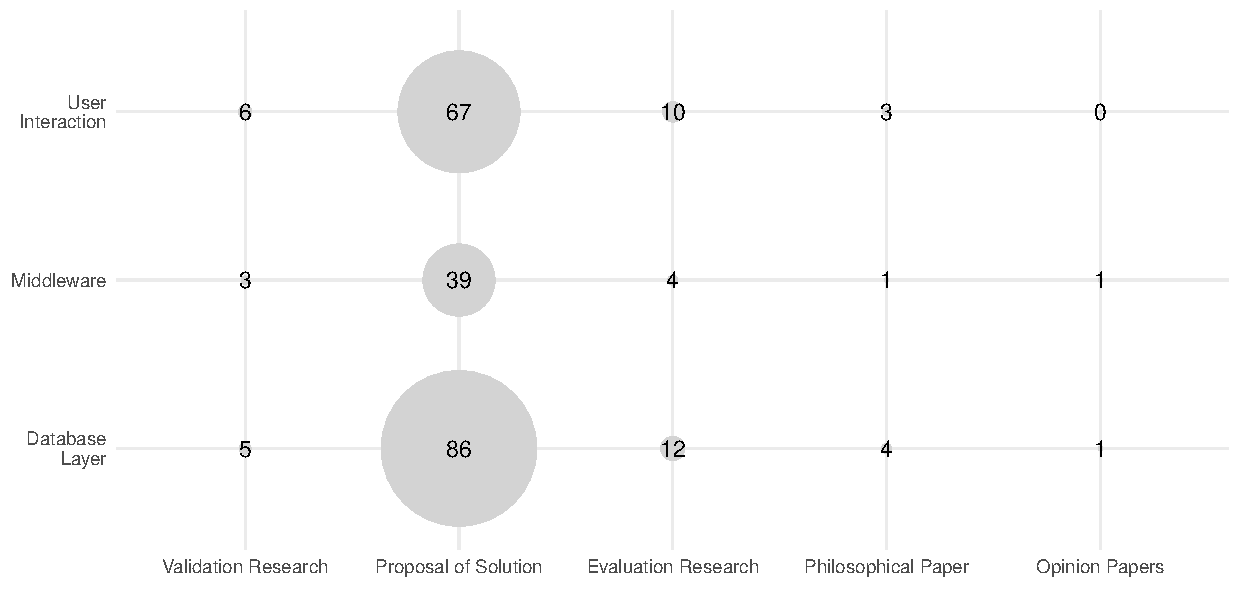
\includegraphics[width=\textwidth]{images/3_mapping/layer_vs_type}
    \caption{\gls{IDE} Layer vs Study research type}
    \label{fig:mapping/layer_vs_type}
\end{figure}

\begin{table}[hptb]
  \small
  \begin{tabularx}{\textwidth}{X r} \hline
    \textbf{Publication} & \textbf{Count} \\ \hline
    \textbf{Journal} & \textbf{55} \\
      \hspace{0.5em} The VLDB Journal & 11 \\
      \hspace{0.5em} IEEE Transactions on Knowledge and Data Engineering & 3 \\
      \hspace{0.5em} IEEE Transactions on Visualization and Computer Graphics & 3 \\
      \hspace{0.5em} International Journal of Cooperative Information Systems & 3 \\
      \hspace{0.5em} Journal of Big Data & 3 \\
      \hspace{0.5em} ACM Transactions on Database Systems & 2 \\
      \hspace{0.5em} Future Generation Computer Systems & 2 \\
      \hspace{0.5em} SIGMOD Record & 2 \\
      \hspace{0.5em} Others & 26 \\
    \textbf{Conference} & \textbf{181} \\
      \hspace{0.5em} ACM International Conference on Management of Data (SIGMOD) & 33 \\
      \hspace{0.5em} Proceedings of the VLDB Endowment & 30 \\
      \hspace{0.5em} IEEE International Conference on Data Engineering & 11 \\
      \hspace{0.5em} Conference on Innovative Data Systems Research (CIDR) & 9 \\
      \hspace{0.5em} Database Systems for Advanced Applications & 5 \\
      \hspace{0.5em} International Conference on Scientific and Statistical Database Management & 5 \\
      \hspace{0.5em} IEEE International Conference on Big Data & 4 \\
      \hspace{0.5em} International Conference on Extending Database Technology & 3 \\
      \hspace{0.5em} International Workshop on Data Management on New Hardware & 3 \\
      \hspace{0.5em} ACM SIGMOD Symposium on Principles of Database Systems (PODS) & 2 \\
      \hspace{0.5em} Advances in Visual Computing & 2 \\
      \hspace{0.5em} Big Data Analytics & 2 \\
      \hspace{0.5em} Database and Expert Systems Applications & 2 \\
      \hspace{0.5em} IEEE International Conference on Mobile Data Management & 2 \\
      \hspace{0.5em} Intelligent Information and Database Systems & 2 \\
      \hspace{0.5em} International Conference on Advanced Cloud and Big Data & 2 \\
      \hspace{0.5em} Workshop on Human-In-the-Loop Data Analytics & 2 \\
      \hspace{0.5em} Others & 62 \\
    \textbf{Gray literature} & \textbf{6}
  \end{tabularx}
  \caption{Frequency of papers by publication forum}\label{tab:mapping/publication}
\end{table}

We refer to our published work~\cite{Alvarez2019} for the complete list of classified publications.

\section{Discussion}
\label{sec:mapping/discussion}

With this results, we now answer the three research questions in
section~\ref{sec:mapping/answers}. Then, in section~\ref{sec:mapping/insights}
we explain the insights we obtain from these answers. Finally,
we enumerate the threats to the validity of this study in
section~\ref{sec:mapping/threats}.

\subsection{Answering the research questions}
\label{sec:mapping/answers}

\subsubsection{RQ1. How has the research area evolved?}
Figure \ref{fig:mapping/layers_histogram} displays the evolution during time
of each of the three major classification clusters: user interaction,
middleware and database.

Considering our search strategy, most of the
results are posterior to 2012. Different approaches seem to be, in general, well
balanced---we refer again to table \ref{tab:mapping/category_summary}---, although there
is space for more works focused on \emph{exploration interfaces} and
\emph{automatic exploration}, which are the less frequent published approaches.

\begin{figure}[hptb]
    \centering
    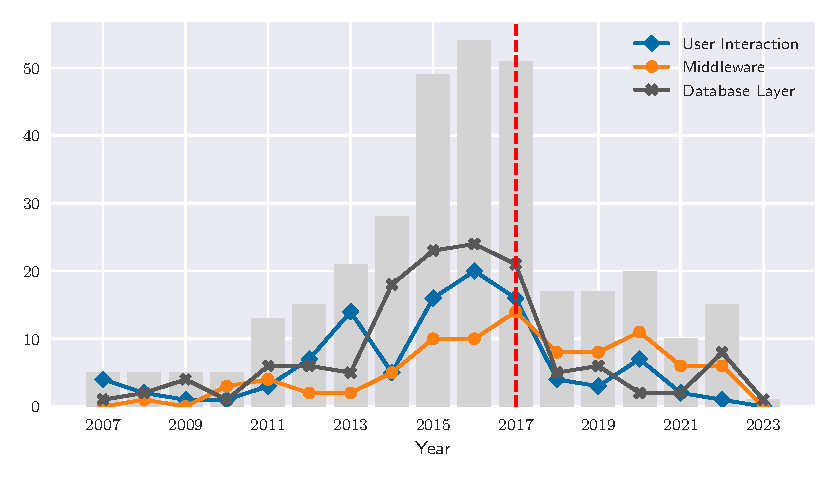
\includegraphics[width=0.6\textwidth]{images/3_mapping/layer_histogram}
    \caption[Number of studies per \gls{IDE} layer and year]{
        Number of papers per layer and year.
        Note that the drop during 2017 is due to the search having been done in May 2017.
    }
    \label{fig:mapping/layers_histogram}
\end{figure}

\subsubsection{RQ2. What is the maturity level of the existing solutions?}
We can use the figure~\ref{fig:mapping/layer_vs_type} to answer this question.
The vast majority of papers considered by this study---79.35\%---fall within the
\emph{proposal of solution} research type.

Meanwhile, \emph{evaluation} and \emph{validation} research are represented
just by a \numprint[\%]{11} and \numprint[\%]{6.07}, respectively.
Only 32 documents (\numprint[\%]{13}) include some sort of user study:
24 for `User Interaction', 4 for `Database  Layer' and 2 for `Middleware'.
Research on how different solutions ---either existing or proposed--- perform in
practice is lacking.

These figures are hardly surprising because they seem to have been commonplace
in computer science for a long time now~\cite{TICHY1995,ZELKOWITZ1997,Sjoberg2005}.
For instance, Sjøberg \etal survey the status of controlled experiments
in software engineering and the numbers they find are equally low, with
only 113 controlled experiments found on \numprint{5 453} papers~\cite{Sjoberg2005}.

It is hard and also out of the scope of this study to make some inferences from these
results. Tichy \etal~\cite{TICHY1995} mention some potential reasons and measures
to improve this situation, namely: difficulty on performing experiments where humans
are involved, the lack of common benchmarks, or even that empirical work is not
encouraged by the journals and conferences of this area.

\subsubsection{RQ3. How far are we from a tool that solves our three requirements?}

\begin{figure}[htbp]
    \centering
    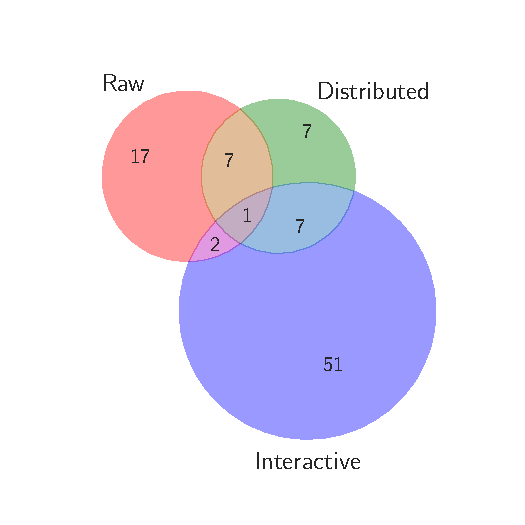
\includegraphics[width=0.5\textwidth]{images/3_mapping/venn}
    \caption{Venn diagram with solutions that satisfy the initial requirements}
    \label{fig:mapping/venn_requirements}
\end{figure}

In figure \ref{fig:mapping/venn_requirements} we display a Venn diagram with our three
requirements. We can see there is a single study that covers the three requirements:
\textit{{A} {D}istributed {I}n-situ {A}nalysis {M}ethod for {L}arge-scale
{S}cientific {D}ata}, by D.Han \etal~\cite{Han2017}. While they mention the
access over raw files and the fact that it is distributed, they do not
explicitly state anything about their interactivity. However, the measured times
for selective queries that they report are in the order of a few seconds. Consequently, we
decided to consider it to be suitable for interactive usage.

The tests they perform use datasets that are close
to the memory available on the system and, therefore, more tests with bigger dataset sizes
could be needed.

Aside from this paper, no other study combines access to raw data with low
response times.

The solutions that cover at least two out of the three requirements are 
summarized in more detail in section~\ref{sec:mapping/details}.

\subsection{Study insights}
\label{sec:mapping/insights}
Research in data exploration is very active and there has been---and there is---
a myriad of solutions proposed. In fact, this should not come as a surprise:
in 2005 Stonebraker~\cite{Stonebraker2005} had already predicted this was bound to
happen and predicted that there would be an increase of domain-specific tools.
This would explain why, of the all classified studies, only one tool satisfies our
three prerequisites.

In general, several different systems and approaches have been proposed, which could,
perhaps, be seen as building blocks. Not all combinations necessarily make sense
but it seems that there are research opportunities in this direction, depending
on the specific needs to be covered.

For instance, in our particular case, we could consider combining distributed
access over raw files, as Han~\cite{Han2017} does, but using approximate query
processing to reduce the response times.

Code generation is a popular approach for querying raw data files
and approximation aware code generation has been noted as a challenge
that is yet to be addressed~\cite{Mozafari2017AQP}. Consequently, more work on this
particular overlap of approaches may provide interesting results.

On a orthogonal consideration, since the generation of data volume will likely
not slow down, the trend for more tools covering specific
niches is probably going to continue. This diversity of tools is a
challenge in itself in many respects, for example: How do we choose the right solution? What is
the cost of making the wrong choice? What happens if the chosen tool goes
unmaintained in the future and there is no community around it? Will it
be hard to maintain? Of course, these questions are not new in software
engineering but typically there are not many choices when it comes to decide
on traditional data storage systems, such as DBMS.
In the last decade, there has been an increase of available options
(relational, object oriented, schema-less, key-value, \ldots) and, while opting
for a DBMS has become harder, it has remained rather manageable. However, looking at the
results of this study, the difficulty for users to decide will likely become
more challenging.

\subsection{Threats to validity}
\label{sec:mapping/threats}
\subsubsection{Search bias}
The gaps identified may be covered in
journals and conferences associated with the user domain---e.g. astrophysics---,
rather than with computer science and engineering. The forward snowballing
step reduces this risk because these hypothetical publications would most likely
cite the original proposal of solution. However, considering that our research method has
allowed us to find even gray literature, we consider this risk to be low.

\subsubsection{Filtering of articles}
Given the huge number of papers that resulted from the search,
a first filtering was done just based on title and abstract.
This is a difficult challenge. Unlike in other disciplines, sometimes abstracts
do not contain enough information about the paper and keywords can be inconsistent
between journals and authors~\cite{Budgen2008,Brereton2007,Jalali2012}.
As recommended by \cite{Brereton2007}, we have also taken into consideration
the conclusions to cover this issue.

\subsubsection{Classification}
Another concern about these classifications is the bias of the researcher's own
interpretation~\cite{MacLure2005}.
For instance, \emph{Jorgensen and Shepperd} report on a disagreement over
39\% of the reviewed papers in their systematic review~\cite{Jorgensen2007}
due to different interpretations of the description of each category. We
have been careful in this respect to guarantee the internal validity of the
study, although some misclassification may still exist.

Additionally, it can be hard to identify if a solution covers or not one of the
three predefined requirements based just on a paper. They may not have been
explicitly mentioned if the authors did not consider them relevant for the
purposes of their publication. Therefore, there may have been false negatives.

The present paper documents our process and the resulting
publication list has been made publicly available---see
section~\ref{sec:mapping/search_strategy}---, so any interested reader can
replicate and/or validate our results.

\section{Discussion of relevant methods}
\label{sec:mapping/details}
Included for completeness is a summary of each of the nine publications 
that cover, at least, two out of the three requirements.

\subsection{All three requirements}
\newcommand{\scidb}[0]{\textsc{SciDB} }

As already mentioned, the only solution that covers the three requirements is
documented on the paper ``A Distributed In-situ Analysis Method for Large-scale
Scientific Data''~\cite{Han2017}, classified as ``adaptive loading''.

The authors build on top of \scidb~\cite{Stonebraker2011}, a distributed
array-based scientific database, and focus on \textsc{HDF} files~\cite{HDF}.
To avoid the overhead of data pre-loading, they leverage the flexible
architecture of this database engine, providing their own scan operator to read
the data directly from the raw files when needed, which needs to be adapted
to the internal representation of \scidb.

This adaptation is done in two different stages: local and global mapping.

During the local mapping, they read on demand the data that matches the filters 
associated to the query, adapting it to the \scidb chunk representation: pieces 
of array data that are distributed together based on some policy - e.g hashing, 
range partitioning.

At the global mapping stage, the resulting chunks are redistributed across the 
storage nodes following the \scidb policies.

Although not relevant for our use case, it is worth mentioning that they also
merge small files together to reduce the performance penalty of processing many
small files.

This approach is interesting as it compartmentalizes well the logic
required to access the raw data from the file distribution and the query engine.

However, the paper notably misses information about the network traffic caused 
by their global mapping stage, since the network overhead depends on how the 
actual data distribution matches \scidb expectations.


\subsection{Distributed access to raw files}
\textbf{\textsc{DiNoDB}}~\cite{Tian2014} is oriented towards the interactive development
of data aggregation algorithms, where the user needs to move quickly between 
the batch processing stage and the interactive evaluation of the quality of 
the results.

It is deployed together with \textsc{Hadoop} and it generates the auxiliary metadata 
using user defined functions executed by the reducers during the batch 
processing stage. Therefore, the metadata ends up stored together with the raw 
data - the output of the reducers, and will also be replicated by the \textsc{Hadoop} 
Distributed File System (\textsc{HDFS}) across the cluster. Additionally, the output 
data may be cached optionally in memory - via ramfs or the filesystem cache.

For the interactive stage, on each HDFS Data Node it is deployed an 
instance of a customized \textsc{PostgresRaw}~\cite{Alagiannis2012Adaptive}
database, a modified version of \textsc{PostgreSQL} with additional support for 
raw files based on positional maps - positions of attributes within the file.

With this architecture deployment, the client 1) issues the query to each 
node separately; 2) \textsc{PostgresRaw} uses the indices to retrieve the offsets of the 
relevant records and the positional maps to find the fields within the 
raw file; and 3) the client aggregates the results.

This approach gets good response times for the interactive stage,
but the latency increases significantly when the output data does not 
fully fit into memory.

\medskip

\textbf{ARMFUL}  (Analysis of Raw data from Multiple Files)~\cite{Silva2017}, 
probably has the most strict requirement set of all the analyzed papers. Its 
authors need to access raw data generated during the execution of a 
workflow and collect their provenance with high granularity. While other 
tools keep track of the data provenance at the file level - leaving to the user 
the cross-match of records stored in different files - they are able to 
associate related data entries contained in the raw data files at the record 
level.

To do so, the authors formally define two additional workflow 
algebraic data operators~\cite{Ogasawara2011}, which allows to address 
specific records stored on a file within a data-flow: \emph{Raw Data Extraction} 
- read, tokenize, filter, parse - and \emph{Raw Data Indexing}. These 
operators can be composed with the existing ones, as \emph{Map} or 
\emph{Filter} - for instance, a user could map a list of file names to their 
content and then filter records with a specific threshold, keeping track of 
the provenance of the data during all the process.

The indexing can rely on external tools, and two implementations are provided:
one based on bitmap indexes generated by FastBit~\cite{Wu2009},
and another one on positional maps, implemented following RAW's 
approach~\cite{Karpathiotakis2014}.

Since this study focus particularly on raw data access during simulations, the 
interactivity only applies to the queries made to the provenance database. 

\subsection{Distributed and interactive}
This combination is the one with the most matching methods. Five 
out of the six ones are classified as ``query approximation'', and the 
remaining one, even though labeled as ``visual optimization'', relies heavily 
on query approximation as well.

It would seem that to get fast responses some compromises on the precision 
have to be made. This makes sense intuitively as processing less 
data will reduce the processing time at the cost of less accuracy. 
Additionally, on a distributed system, some nodes may be offline, 
unresponsive or overloaded. In order to keep the latency low, the results 
need to be aggregated within a reasonable deadline, even if parts of the system 
have not responded yet.

It is worth noting that most of these papers also match the ``sampling''
category, but since sampling is just an aspect of the overall solution and their 
authors normally use ``query approximation'' to refer to their methods, we have 
decided to classify them as such.

\medskip

\textbf{BlinkDB}~\cite{Agarwal2013} allows users to perform SQL-like aggregation 
queries on data stored on HDFS, specifying time or error constraints. First, 
the authors base their system on the assumption - supported by evidence - that 
the column sets used for the aggregation queries are predictable, regardless of 
the actual grouping value. With this information, they perform a stratified 
sampling~\cite{Lohr2009} to avoid the under-representation of rare subgroups. 
Finally, the system chooses the suitable samples based on the query constraints 
provided by the user, profiling them at run time so it can improve the 
execution plan for later queries.

\medskip

\textbf{ScalaR}~\cite{Battle2013} improves the performance of the visualization 
of big data sets dynamically reducing the size of the response returned to the 
front-end layer. Its authors provide an intermediate layer that consumes the 
queries issued by the user and uses the statistics computed by the database 
back-end to evaluate in advance the expected size of the result set. If this 
size is above a given threshold, the query is rewritten to either aggregate, 
sample or filter the data, generating a smaller approximate response that can be 
displayed more performantly.

Although their solution is back-end agnostic, their proposed implementation 
relies on \scidb~\cite{Stonebraker2011}. It quickly comes to mind that this could 
potentially be integrated with the previous method by Han \etal~\cite{Han2017}, 
resulting on a visual exploration tool for raw data files.

\medskip

The authors of \textbf{DICE} (Distributed and Interactive Cube 
Exploration)~\cite{Kamat2014} attack the problem on three fronts: speculative 
query execution, online data sampling, and an exploration model - 
\textit{faceted} cube exploration - that limits the number of possible queries, 
improving the efficacy of the speculative execution.

Probably, the most interesting idea from this paper is the notion of 
the exploration being done in ``sessions'': The authors do not attempt to 
optimize for any possible query, but only for those that are likely to follow 
from the state of the current session. Predicting a set of potential following 
queries is made possible thanks to their exploration model, which
restricts the possible number of ``transitions'' from the current state 
for a session.

The predicted queries are then ranked based on their likelihood and 
accuracy gain, and those that are most likely and provide the most accuracy gain 
will be speculatively executed in advance, populating the cache. When the final 
query arrives, the response can be built from the content of the cache if the 
predictions were successful. Otherwise, it will be scheduled to the underlying 
nodes.

For more information about ``data cubes'', we refer to the DICE paper,
or the original proposal~\cite{Gray1997}.

\medskip

\textbf{AccuracyTrader}~\cite{Han2016} is a distributed approximate processing 
system comprised of two components: one online and one offline.

First, the offline part reduces the dimensionality of the original data using 
Single Value Decomposition - so it only supports numerical values. 
Then, it groups similar entries using an R-Tree, where each node represents an 
aggregated data point, and all nodes at the same level correspond to a 
``synopsis''. This tree is flattened into an index at a level that balances 
between the number of leaves under each aggregated data point and the 
selectivity of the tree at that level. Finally, it aggregates the data for 
each index entry using the original dimensions of the indexed points and stores 
this aggregated data into the ``synopsis''.

When a query arrives, the online part uses these ``synopsis'' to produce 
an approximate result with an accuracy estimation. It then iterates 
using the detailed data points to improve the response accuracy until the
deadline specified by the user expires.

In this paper, the authors prove that the system scales well in terms 
of tail latency and accuracy when the number of requests increases for a 
``search engine''-like workload. However, the data has to be aggregated into 
the synopsis beforehand.

\medskip

\textbf{KIWI}~\cite{Kim2015} is a SQL front-end built on top of Hadoop that aims 
to provide both batch processing and interactive analytics via approximate
query processing. It generates both vertical (column) and horizontal (row) 
samples, and re-writes the queries to use these samples instead of the original 
data. However, it is hard to assess the technical soundness of this 
solution, since the paper is very short - 2 pages including citations -
and we have not been able to find any later citations nor do the authors cite 
other papers about the same tool.

\medskip

Finally, Wang \etal~\cite{WangYi2015} introduce a framework based on the 
map-reduce paradigm. Instead of the traditional batch processing approach 
where the analysis is performed on big chunks of data, their system executes the 
analysis logic iteratively on samples, updating an estimator in each round 
until a stop condition is satisfied - both estimator and condition provided by 
the user. When the termination condition is satisfied, the remaining jobs are 
canceled, saving computing cycles and reducing the latency. Similarly to other 
analyzed solutions, they use a stratified sampling to ensure a good accuracy and 
the coverage of rare cases. 
The sampling is done without replacement, so in each iteration new data points 
are taken into account, improving the selectivity of the method.

\subsection{Summary}
We can see some commonalities looking at the underlying techniques used by the 
solutions described above:

First, for providing access to raw files, code generation and positional 
mapping seem to provide a good solution. Both are implemented either directly - 
PostgresRaw - or used via integration with an existing implementation - DiNoDB. 
Isolating the raw data access as a database operator composes well for all 
studied solutions regardless of the framework of reference - workflow, 
PostgreSQL or \scidb.

Second, to provide the interactivity on a distributed system, the engine 
needs to approximate the results using a deadline or an accuracy requirement as 
a stop condition. The resiliency and the low latency are achieved by 
being capable of processing only parts of the data, via sampling - BlinkDB -, 
pre-computed summaries - AccuracyTrader - or both. In either case, error 
estimation becomes an important part of the system, both internally and as 
part of the interface exposed to the user.

\section{Conclusions}
\label{sec:conclusions}
In this systematic mapping study we have detailed the method that we followed
to gather and filter papers related to \emph{data exploration}, searching
for solutions that tackle big data volumes, stored in a distributed way and with
a low latency. This process have produced 242 papers, which we have classified
according to their approach~\cite{Idreos2015} on one axis, and to their research
type~\cite{Wieringa2006} on another.

The results suggest that  plenty of solutions have been proposed by researchers.
However, there is rarely any follow up, at least published, on their
practical implementation, be it to confirm a successful introduction to users
or to evaluate other tools already in place.
Unfortunately, this is not different to the state of other areas of the computing sciences.

We have found evidence that code generation is a well-proven approach for
accessing raw data files, although most solutions have not been generalized
onto a distributed environment.



\chapter{Identifying gaps}
\label{chapter:diverse}
As a result of the survey presented in chapter~\ref{chapter:literature_review},
we realized that most solutions treat files
as separate, independent, relations, leaving it to the end-user to work out how they are related,
an observation shared by other authors~\cite{Silva2016}.
These files may have not yet been ingested into a database system and 
the schema may be unfamiliar and not adequately documented, or even be
composed of multiple files with heterogeneous schemes~\cite{alawini2016,zhang2015astronomy}.
We consider that Idreo's classification misses a category for this problem:
\emph{Schema Homogenization}. This new category belongs to the \emph{Middleware} layer.

In \emph{Data Mining in Astronomical Databases}, Borne
describes how data exploration of this kind of diverse datasets is
relevant since it can drive serendipitous discoveries~\cite{Borne2001}. He proposes
two groups of data mining approaches in this respect: event
based and relationship based:

\begin{itemize}
    \item \textbf{Event based}
        \begin{itemize}
          \item \emph{Known events / known algorithms}
            Use physical models to locate known phenomena of interest spatially
            or temporally within a large database.
          \item \emph{Known events / unknown algorithms}
            Use pattern recognition and clustering to discover new relationships between known
            phenomena.
          \item \emph{Unknown events / known algorithms}
            Use predictive models to predict the presence of unseen events within a
            large and complex database.
          \item \emph{Unknown events / unknown algorithms}
            Use thresholds to identify transient or unique events.
        \end{itemize}

    \item \textbf{Relationship based}
        \begin{itemize}
            \item \emph{Spatial}
                Identify objects in the same location.
            \item \emph{Temporal}
                Identify events occurring within the same time period.
            \item \emph{Coincidence}
                In general, apply clustering techniques to
                identify objects that are co-located within a multidimensional space.
        \end{itemize}
\end{itemize}

Borne then enumerates a list of science requirements for data mining:

\begin{itemize}
    \item \emph{Object Cross-Identification} between catalogs. Similar to the natural join
        in relational algebra, but based on spatial or multidimensional co-location.
    \item \emph{Object Cross-Correlation} comparing sets of attributes over the full set of objects.
        For instance, identify remote galaxies as those that are \emph{not} present on
        the ultraviolet spectrum.
    \item \emph{Nearest-neighbor identification} or, in general, application of clustering
        algorithms in multidimensional spaces.
    \item \emph{Systematic Data Exploration} via event- and relationship-based queries to a database
        hoping to make serendipitous discoveries.
\end{itemize}

Following the methodology described in chapter 2, we have identified an essential problem:
exploring multiple files with uncertain numerical data is a neglected aspect in the \gls{IDE}.
With this insight, we have returned to the clarification stage and used Borne's description
of data exploration in astronomy to better understand data exploration in
this context.


In section~\ref{sec:real_use_cases} we use an existing astronomy database
to expand our understanding of how users explore datasets. Then,
in section~\ref{sec:objectives} we refine and concretize the objectives
of the present thesis. In section~\ref{sec:gaps/principles} we identify
solution principles from the literature. Finally, in
section~\ref{sec:gaps/proposed}, we list two proposals of solution and refer
to the respective chapters that document them.

\section{Examining real use cases}
\label{sec:real_use_cases}

We looked for concrete examples of queries mentioning \emph{astronomy} on the
242 articles classified on the systematic literature mapping from
chapter~\ref{chapter:literature_review}.

It is soon evident that the \gls{SDSS}~\cite{SDSS14} is popular as a test
set since it is readily available and well documented~\cite{Gray2002}.
Furthermore, there are easily accessible sample queries~\cite{SDSSSamples}
and real ones~\cite{SDSSSqlLogs}.
Listing~\ref{sql:get_queries} shows an example of how to obtain a list
of queries performed by users.

\begin{listing}[htbp]
\begin{minted}[linenos]{sql}
    SELECT clientIP, seq, statement, elapsed
    FROM SQLlog
    WHERE yy=2018 AND mm>=10 AND rows>0 AND dbname LIKE 'BestDR14%'
\end{minted}
\caption[Obtaining a list of queries performed by \glsentrylong{SDSS} users]{
    Example of how to obtain a list of queries performed by users during the end of 2018 over the 14th data release.
}\label{sql:get_queries}
\end{listing}

In total, 25 articles ($10.3\%$) use \gls{SDSS} as a test dataset.
Table~\ref{tab:sdss_queries_count} classifies these 25 articles following the same schema as described
in section~\ref{sec:mapping_category}.

\begin{table}[htbp]
  \begin{center}
    \begin{tabular}{l r r r}
      \textbf{Category} & \textbf{Total} & \textbf{SDSS} & \textbf{\%} \\ \hline
      Exploration Interfaces & 34 & 3 & $8.8\%$ \\
      Indexes & 58 & 5 & $8.6\%$ \\
      Storage & 39 & 11 & $28.3\%$ \\
      Data Visualization & 36 & 2 & $5.6\%$ \\
      Interactive Performance Optimizations & 48 & 4 & $8.3\%$ \\
    \end{tabular}
  \end{center}
  \caption{Classification of the articles that use the data from the \glsentrylong{SDSS}}\label{tab:sdss_queries_count}
\end{table}

To obtain an overview of the type of usual utilization of this database, we processed
the results from query~\ref{sql:get_queries}. We extracted the columns, relations,
and filters usually affected by the queries.
Table~\ref{tab:most_tables} shows the most frequent queried combinations
of relations.

\begin{table}[htbp]
\centering
\begin{tabular}{l r r}
    \textbf{Tables} & \textbf{Count} & \textbf{Percentage} \\ \hline
    fGetNearbyObjEq, PhotoPrimary          &  264785 &  37.62\% \\
    DBObjects\textdagger         &  150458 &  21.37\% \\
    PhotoTag, fGetObjFromRectEq            &   93094 &  13.23\% \\
    IndexMap\textdagger          &   41265 &   5.86\% \\
    Galaxy, fGetNearbyObjEq                &   31130 &   4.42\% \\
    sppParams, PhotoTag, fGetObjFromRectEq &   29805 &   4.23\% \\
\end{tabular}
\caption[Most frequently queried relations from the \glsentrylong{SDSS}]{
    Combination of relations most frequently queried. Tables marked with (\textdagger)
    are meta-data tables (i.e., describe the schema)
}\label{tab:most_tables}
\end{table}

Interestingly, introspection queries are widespread, indicating that
users spend a considerable time familiarizing themselves with a complex schema.
This has led to attempts at reducing this friction by methods such as context-aware auto-completion~\cite{Khoussainova2010}.

\section{Refining objectives}
\label{sec:objectives}

We summarize here our insights after the literature survey and examination
of real use cases:

\emph{Support for data distributed across multiple files} is generally neglected by
\emph{in-situ} data exploration solutions~\cite{Silva2016,alawini2016}.
However, indexing, storage, and
interactivity are well covered, as seen in chapter~\ref{chapter:literature_review}.

\emph{Exploring the database schema} itself, as the \gls{SDSS} query logs suggest, is
non-negligible user activity. Our observation is consistent with an IBM study that finds
that even data architects can spend up to 70\% of their time just discovering the metadata of
databases~\cite{Wu2008}.

Our refined question is: can we help users to navigate datasets split across multiple
files, with unknown schema, facilitating relationship-based mining?
We can rely on name matching when metadata is present, but what can be done when
it is missing, or if correspondences are not unambiguous?

\section{Solution principles}
\label{sec:gaps/principles}

Our use case looks like the following: an astronomer facing several
data files containing raw astronomical measurements
with little or no explanation about their schema. These files may come from different
surveys or different sets of observations from the same region of the sky,
and the user can only make the following educated guesses:

\begin{itemize}
    \item The populations are likely the same, or at least very similar
    (i.e., stars).
    \item A subset of the attributes is shared between the relations (i.e.,
    brightness on different electromagnetic bands).
    \item The measurements have an associated uncertainty~\cite{Stonebraker2009},
    either explicitly stated or not (i.e., random errors, instrument precision,
    floating point precision).
\end{itemize}

To help cross-matching the files, the first intuition would be to run a statistical
test between all possible pairs of columns,
such as the Kolmogorov-Smirnov~\cite{Hodges1958} or Wilcoxon~\cite{Wilcoxon1945} tests.
However, as figure~\ref{fig:pairwise_ind} exemplifies, this information is not enough to 
do a cross-match.

\begin{figure}[htpb]
    \centering
    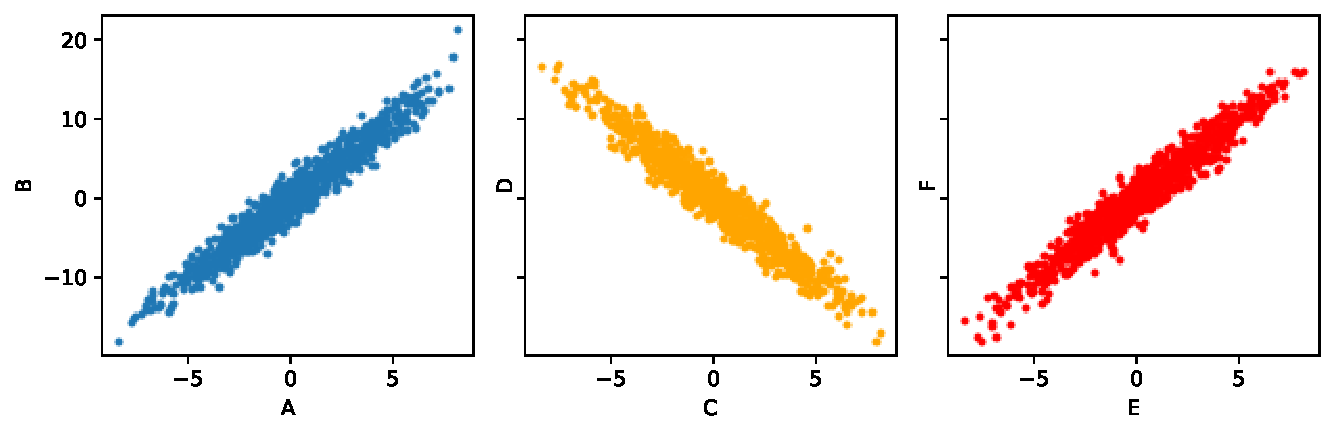
\includegraphics[width=\linewidth]{images/4_gaps/no2ind}
    \caption[Example of a 2D distribution where the pairwise matching is not enough]{
        Example of a 2D distribution where the pairwise matching would not be accurate enough.
        Pairwise tests would tell us that $A$ matches $C$ and $E$; and that $B$ matches $D$ and $F$.
        However, $A,B$ does not match $C,D$.
    }
    \label{fig:pairwise_ind}
\end{figure}

Therefore, a solution to our research question must take multidimensionality into account.

To bridge this gap, we propose the concept of \glspl{EDD}, which is inspired by the idea of
\glspl{IND} from the relational algebra:

\begin{displayquote}
An inclusion dependency between column A of a relation
R and column B of a relation S, written $R.A \subseteq S.B$, or $A \subseteq B$
when the relations are clear from the context, asserts that each
value of A appears in B. Similarly, for two sets of columns X
and Y , we write $R.X \subseteq S.Y$ , or $X \subseteq Y$ , when each distinct
combination of values in X appears in Y \cite{abedjan2015}
\end{displayquote}

The definition of \gls{IND} is based on set theory, which is not directly applicable to
numeric data where measures are in the real domain (e.g. spatial coordinates
or flux measurements) and usually
have an associated uncertainty that may or may not be explicitly stored.

However, this definition can be naturally reformulated in terms of
equality of distribution $X \eqdist Y: F_X(x) = F_Y(x) \; \forall x$, where $F_X$ and
$F_Y$ are the cumulative distribution functions of X and Y, respectively:

\begin{definition}
An equally-distributed dependency between a set of columns X from
of relation R and a set of columns Y of relation S, written $R.X \eqdist S.Y$ or
$X \eqdist Y$ asserts that the values of X and Y follow the same probability distribution.
\label{def:eqdist}
\end{definition}

The term \emph{arity} refers to the cardinality of the sets of attributes $X$ and $Y$. For instance, if $|X| = 1$, we talk about unary \glspl{EDD}; if $|X| = 2$,
binary or 2-\glspl{EDD}; and, in general, for $|X| = n$, $n$-ary \glspl{EDD}.

Finding high arity \glspl{IND} is an NP-hard problem~\cite{kantola1992}.
For instance, for two sets of $n$ attributes in $R$ and $S$,
there are $n!$ different possible permutations to check.
In comparison, finding unary \glspl{IND} seems a relatively simple problem,
as the worst case has complexity $O(n^2)$. Nonetheless,
testing over real files may require expensive input/output operations.
Furthermore, as we will see later, false positives at this stage can quickly make
finding high arity \glspl{IND} unfeasible. This is because the search space tends to grow exponentially
with the number of one-attribute matches, making unary \glspl{IND} search time much less important
than reducing the number of false positives.

We used a published experimental evaluation of \gls{IND} finding techniques~\cite{Dursch2019} as a starting point for
assessing how adequate existing solutions are for our problem. The authors carried out a
set of experiments with thirteen \gls{IND} algorithms, of which seven are for unary \glspl{IND},
four for $n$-ary \glspl{IND}, and two for both types. A more recent survey confirms that this
work contains the current state-of-the-art for Inclusion
Dependencies~\cite{kossmann_data_2022}.

We will now describe briefly the $n$-ary finding
algorithms evaluated by the authors and discuss their suitability for our needs.

\subsection{n-IND finding algorithms}
\label{sec:nind_finding}
\begin{figure}[ht]
    \centering
    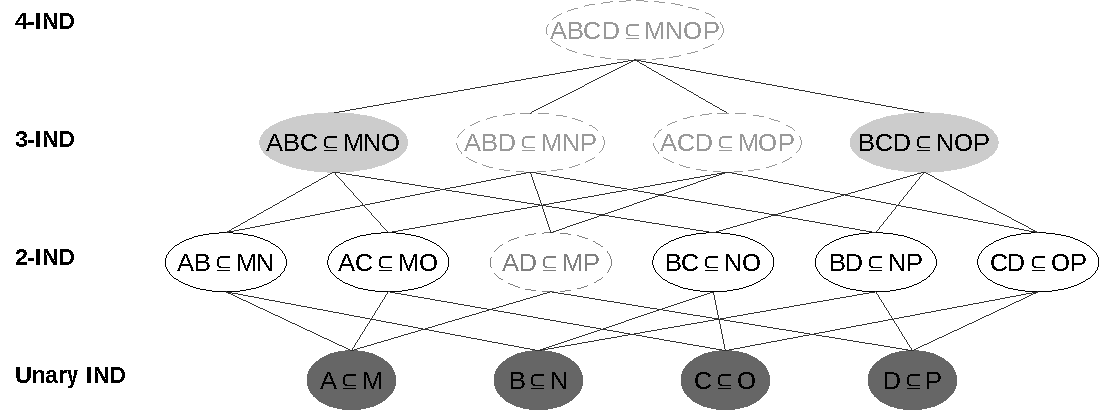
\includegraphics[width=\linewidth]{images/5_presq/lattice}
    \caption[Example structure of the search space as a lattice for an initial set
        of 4 unary \glslongpluralkey {IND}.]{
        Example structure of the search space as a lattice for an initial set
        of 4 unary \glspl{IND}.
        As an illustration, if the 2-INDs surrounded by a solid line were valid,
        a bottom-up traversal would only need to check the validity of the 3-INDs with a 
        gray background since the others could not be valid.
    }
    \label{fig:lattice}
\end{figure}

Given two relations $R$ and $S$, with attributes A and B respectively,
a unary Inclusion Dependency (uIND) exists if $R.A \subseteq S.B$.
More generally, for two sets of attributes $X$ and $Y$, both of cardinality $n$, an
$n$-ary Inclusion Dependency (nIND) exists if every combination of values in X appears in Y
\cite{DeMarchi2002,abedjan2015}.

Given a set $U$ of valid uINDs, the search space for
higher-arity candidates is defined by its power set and a partial order relation
called specialization~\cite{DeMarchi2002}:

\begin{definition}
    \label{def:specialization}
    Let $I_1 = R[X] \subseteq S[Y]$ and
    $I_2 = R'[X'] \subseteq S'[Y']$. $I_1$ \textbf{specializes} $I_2$ (denoted $I_1 \prec I_2)$ iff
    
    \begin{enumerate}
        \item $R = R'$ and $S = S'$.
        \item $X$ and $Y$ are sub-sequences of $X'$ and $Y'$, respectively.
    \end{enumerate}
    
    We can also say that $I_2$ \textbf{generalizes} $I_1$.
\end{definition}

\begin{example}
$(R[AB] \subseteq S[EF]) \prec (R[ABC] \subseteq S[EFG])$. However,
$R[AB] \subseteq S[DE]) \nprec (R[ACD] \subseteq S[DFG])$
\end{example}

This partial order enables us to structure the search space as a lattice, as exemplified in figure
\ref{fig:lattice}. Most solutions leverage this property to explore the search space bottom-up
---from level $k$ to $k$+1--- or top-down ---from level $k$ to $k$--1--- order.

\textsc{Mind}~\cite{DeMarchi2002} is a bottom-up approach: it starts
from a set of known, satisfied unary \glspl{IND} and builds higher arity candidates
combining them.
These new candidates are then validated against the database, and those satisfied
are used for computing the next-level candidates until no more candidates are available.

\Zigzag~\cite{DeMarchi2003zigzag} starts with a \textsc{Mind} bottom-up approach
up to a given arity $n \ge 2$. Then, it uses all satisfied \glspl{IND} to initialize a \textit{positive border}
and the non-satisfied to initialize a \textit{negative border}. The set of satisfied \glspl{IND}
is used to generate the set of candidates with the highest arity possible, called
\textit{optimistic border},
which is then validated against the database. This is the bottom-up part of the search.
Valid candidates are directly added to the positive border.
Invalid candidates are treated depending on how many tuples are different between relations.
Those above a given threshold (too many different tuples) are added to the negative border.
Those below are top-down traversed, from level $n$ to $n$--1, validated, and then added
to the positive border if they are satisfied. The algorithm then iterates, building a new
optimistic border until it is impossible to generate new \glspl{IND}. The optimistic approach
can prune the search space very aggressively when there are high-arity \glspl{IND},
but when most arities are low,  \textsc{Mind} may perform better.

\Find~\cite{koeller2003discovery} is based on the equivalence
between finding $n$-INDs and finding cliques on $n$-uniform hypergraphs (a generalization
of the concept of a graph where each edge connects $n$ nodes). Each unary \gls{IND} corresponds
to a node, and an $n$-IND corresponds to an edge on an $n$-uniform hypergraph.
Once such a graph is built, each \gls{IND} corresponds to a clique and maximal \glspl{IND}
correspond to maximal cliques. They present the \Hyperclique algorithm,
capable of finding maximal cliques performantly, which can be mapped back to candidate
maximal \glspl{IND}. These are finally validated using database queries.
As \Zigzag, \Find starts with a bottom-up
approach to look for maximal cliques (i.e., potential maximal \glspl{IND}). The invalid ones
are used to generate a new ($n$+1) uniform graph. This is a stage that corresponds to the top-down
traversal.

While these three algorithms were evaluated on \glspl{IND} between relational datasets
and with attributes that can be directly compared (i.e. from discrete domains), their
traversal of the search space and their validation steps are well decoupled. They
can be easily be adapted to the equality-of-distribution statistical tests.

Furthermore, the reference benchmark shows that \Mind, \Find
and \Zigzag have a comparable run-time, sometimes even
faster than the alternatives.
While \textsc{Faida} is generally faster, its
validation strategy requires computing hashes over the
attributes and their combinations, which is inapplicable
for continuous data that can very possibly have an associated uncertainty.

From the three suitable candidates, \Mind's bottom-up approach can be performant enough for
relatively low arity \gls{IND} relations. However, it has one substantial disadvantage:
it requires an exponential number of tests, prohibitive for higher arity \glspl{IND}.
Both \Zigzag and \Find overcome this limitation by alternating between \emph{optimistic}
(top-down) and \emph{pessimistic} (bottom-up) traversals.
Finally, \Find maps the search of \glspl{IND} to the search of maximal cliques. We know that
using statistical tests will introduce unavoidable false negatives, which would
translate into missing edges.
A clique with missing edges is a quasi-clique, and finding quasi-cliques, while at least
as hard as finding cliques, is doable.

\subsection{Foreign Key Discovery}

We briefly survey this area since we consider it complementary to
\gls{IND} discovery. A \gls{FK} constrain on an attribute
$A$ over a \gls{PK} $B$ implies that all values present on $A$ must also be
present on $B$.
Therefore, there exists an inclusion dependency between $A$ and $B$.
However, the reverse is not necessarily true. For instance, two auto-increment attributes from
two different relations may have an accidental \gls{IND} with no semantic meaning.

To distinguish between accidental and meaningful \glspl{IND}, Rostin \etal~\cite{Rostin2009} propose to
train machine learning models over a set of features extracted from positive
\gls{PK}/\gls{FK} relations and negative, non-meaningful \glspl{IND}. However, their proposal
is limited to unary \glspl{IND}.

Zhang \etal~\cite{Zhang2010} present an algorithm capable of handling multi-column
\gls{PK}/\gls{FK} relations.
They define the concept of \emph{Randomness Test}, which assumes that an \gls{FK} is a representative
sample of a \gls{PK} and, therefore, should follow a similar distribution.
They use an approximation of the \gls{EMD} ---the cost of transforming one distribution into another---
to measure the similarity between \gls{PK} and \gls{FK}.
Their algorithm ranks \gls{PK}/\gls{FK} candidates by distance ---closest first--- and selects
the top $X\%$, where $X$ must be chosen to balance precision and recall.

More recently, Jian \etal~\cite{jiang_holistic_2020} introduced an approach that identifies
both \gls{PK} and \gls{FK} holistically. They validate Zhang's concept of \emph{Randomness}
and propose a simplified estimator that treats each attribute separately. They do not need
the \glspl{PK} to be known but require a list of \glspl{IND} as input.

It is worth noting that even though the latter two publications use the idea of the
\gls{FK} being a random sample of the \gls{PK}, their methods use the \emph{distance} between
distributions for ranking candidates~\cite{Zhang2010} or as a feature~\cite{jiang_holistic_2020}.
Our method is based, however, on statistical hypothesis testing\footnotemark.

\footnotetext{While the \gls{EMD} could be used as a test statistic, it would be computationally
expensive~\cite{hallin2021multivariate}.}

\subsection{Complementarity}

\textsc{ReDiscover}~\cite{alawini2016} uses machine learning techniques, such as
\glspl{SVM}, to identify matching columns between scientific tabular data.
The author defines different ways in which datasets may be related:
containment, partial containment, augmentation, completion, equality, \ldots
This solution focus does not only focus on correspondences (i.e., $A$ is a subset of $B$),
but it also pays attention to the semantics of the \emph{relationship} (i.e., $A$
is a selection of $B$).
Yet, this system focuses mainly on the correspondence between \emph{individual columns},
which is insufficient for spatial and coincidence associations, as they are multidimensional.
We are left only with a set of pairwise correspondences that may not be enough to cross-match
tuples between files.

\subsection{Schema Homogenization}
\label{sec:schema_homogeneization}

For completeness, table~\ref{tab:missing_middleware} classifies these solutions
under the proposed \emph{Schema Homogenization} category,
expanding on the result from the literature mapping shown in chapter~\ref{chapter:literature_review}.

\begin{table}[ht]
    \centering
    \begin{tabularx}{\linewidth}{p{7em} >{\raggedright}X >{\raggedright}X X}
    \hline
    \multicolumn{4}{l}{\textbf{Middleware}} \\
    \hline
    \textit{Schema \mbox{Homogenization}} &
    \gls{IND}     \cite{DeMarchi2002,DeMarchi2003zigzag,koeller2002integration} &
    \gls{FK}      \cite{Rostin2009,Zhang2010,jiang_holistic_2020} &
    Complementarity \cite{alawini2016} \\
    \hline
    \end{tabularx}
    \caption[Articles under Schema Homogenization]{
    Expansion of Idreos~\cite{Idreos2015} classification with \emph{Schema Homogenization}}
    \label{tab:missing_middleware}
\end{table}


\section{Proposed solution}
\label{sec:gaps/proposed}
In the following chapter, we propose a novel algorithm, \PresQ, that
can recover multidimensional correspondences between datasets with different,
undocumented --- or unknown --- schemas. \PresQ relies on statistical tests to
accept or discard these correspondences.

To complement this method, chapter~\ref{chapter:som} describes a multidimensional
statistical test based on \gls{SOM} offering additional interpretability. It can be
used with \PresQ for studying with more details accepted or rejected correspondences,
or afterward over the merged dataset for clustering or as a pre-processing for nearest-neighbor
coincidence search~\cite{silva2011som}.

Appendix~\ref{appendix:prototypes} briefly describes the preliminary ideas that were
discarded during the phase of \emph{Embodiment Design}.


\chapter{Discovery of Multidimensional Dependencies via Quasi-Cliques on Hypergraphs}
\label{chapter:presq}
\glsresetall

Most of the content in this chapter appears in the article
\emph{\textsc{PresQ}: Discovery of Multidimensional Equally-Distributed Dependencies via Quasi-Cliques on Hypergraphs}~\cite{AlvarezAyllonPresQ2022},
published on \emph{IEEE Transactions on Emerging Topics in Computing}.

\medskip

\PresQ is a statistically robust algorithm for finding \glspl{EDD}, as described
in definition~\ref{def:eqdist}.

Following the \emph{Engineering Design} process, \PresQ is the \emph{output} of
the \emph{embodiment design} phase of the design process, and the present chapter
is its documentation.
In section~\ref{sec:presq_definitions}, we list the set of rules needed to be able
to define a search space for \glspl{EDD} and introduce the concepts of
hypergraph and quasi-clique. In section~\ref{sec:presq_inferring}, we propose
a novel algorithm based on quasi-cliques to infer common equally-distributed
multidimensional attributes.
In section~\ref{sec:presq_experiments}, we show experimental results
that prove that \PresQ successfully finds dependencies in a reasonable amount of time.
Finally, in section \ref{sec:presq_conclusions}, we compile the conclusions and
propose areas for further work.

\section{Definitions}
\label{sec:presq_definitions}

\subsection{Equally Distributed Dependencies}
\label{sec:edd}
An Inclusion Dependency exists if all combinations of
values from a given set of attributes in one relation are contained within
a set of attributes from another.
However, we will hardly ever find a strict
subset relation between two attributes in the real domain. Measurements may have associated uncertainty,
and even floating-point representation may vary (i.e. 32 vs 64 bits). It is generally a
flawed idea to compare floating-point numbers with strict equality.

Instead, we can use $R.X \eqdist S.Y$ as an approximation, meaning that the two sets of
attributes are equally distributed. This relation is, unlike the subset relation, symmetrical.

Following the parallelism with \gls{IND} finding, we say that the dataset $d$ satisfies
the relation defined by equality of distribution $\eqdist$ when a statistical test
fails to reject the null hypothesis
\begin{equation}
    H_0: P(R[X]) = P(S[Y])
    \label{eq:eqdist}
\end{equation}
Three inference rules can be used to derive some additional \glspl{IND} from an already known
set of \glspl{IND}. They are defined using sets and subsets \cite{Casanova1984},
but they translate to the equality of distribution:

\begin{description}
    \item[Reflexivity] \hfill \\
        $R[X] \eqdist R[X]$
    \item[Permutation and projection] \hfill \\
        If $R[A_1,\dots,A_n] \eqdist S[B_1,\dots,B_n]$ then
        $R[A_{i_1},\dots,A_{i_m}] \eqdist S[B_{i_1},\dots,B_{i_m}]$ for each sequence
        $i_1,\dots,i_m$ of distinct integers from $\{1,\dots,n\}$
    \item[Transitivity] \hfill \\
        $ R[X] \eqdist S[Y] \land S[Y] \eqdist T[Z] \implies R[X] \eqdist T[Z]$
\end{description}

The reflexivity, permutation, and transitivity rules are well-known to hold
for $\eqdist$ \cite{randles1979introduction}.

%We have proven that the projection rule also holds, as is logical~\cite{Alvarez2021inference}.
For the projection, we need to prove that if two sets of random variables
$X_1,\dots,X_n$ and $Y_1,\dots,Y_n$ are equally distributed, so are
any of their possible sub-sequences.

\begin{proof}
Let $X'$ and $Y'$ be the sequences $X_1,\dots,X_m$ and $Y_1,\dots,Y_m$ with $m < n$.
Their corresponding  \gls{CDF} are just the \emph{marginal} \gls{CDF}:

\begin{equation}
\begin{split}
    F_{X_1,\dots,X_m}(x_1,\dots,x_m) = & F_{X_1,\dots,X_m,X_{m+1},X_n}(x_1,\dots,x_m,x_{m+1},\dots,x_n) \\
    F_{Y_1,\dots,Y_m}(y_1,\dots,y_m) =& F_{Y_1,\dots,Y_m,Y_{m+1},Y_n}(x_1,\dots,x_m,x_{m+1},\dots,x_n)\\
    & \forall (x_1,\dots,x_m) \in \mathbb{R}^m \textrm{ and } x_i \xrightarrow{} \infty \; \forall i > m
\end{split}
\end{equation}

By definition \ref{def:eqdist}, the right hand-side of both equations must be the same.
By transitivity, 

\begin{equation}
\begin{split}
    & F_{X_1,\dots,X_m}(x_1,\dots,x_m) = F_{Y_1,\dots,Y_m}(y_1,\dots,y_m) \\
    & \implies X_1,\dots,X_m \eqdist Y_1,\dots,Y_m
\end{split}
\end{equation}

\end{proof}

Thanks to the validity of these rules, particularly the permutation and projection,
we can use the specialization relation seen in definition \ref{def:specialization}
when dealing with distributions.

With these rules we have defined the search space similar to the one from \gls{IND} discovery.
The last requirement is a property that allows the pruning of the
search space as illustrated in figure~\ref{fig:lattice}.

Let $I = R[X] \eqdist S[Y]$.
A dataset $d$ \emph{satisfies} $I$ iff  a statistical test fails to reject $H_0: P(R[X]) = P(S[Y])$
given a significance level $\alpha$.
This is denoted as $d \models I$.

\begin{property}
    Given $I_1 \prec I_2$:
    
    \label{prop:prob_spec}
    \begin{enumerate}
        \item If $d \models I_2$, then $d \models I_1$ (Accepting $H_{0_2}$ implies accepting $H_{0_1}$\footnotemark)
        \item $d \not\models I_1$ with a probability $\alpha$ when $d \models I_2$
            (Rejecting $H_{0_1}$ \emph{does not} imply the rejection of $H_{0_2}$)
    \end{enumerate}
\end{property}

\footnotetext{Strictly speaking, \emph{not rejecting} $H_{0_2}$ implies that we can not reject $H_{0_1}$.}

This property is similar to that proposed for \glspl{IND}~\cite{DeMarchi2002}, with the exception that even if $d \models I_2$, there is a probability to falsely reject $I_1$ bound by the significance level $\alpha$.

\begin{example}
    If we have two sets of $10$ attributes that are equally distributed, the number of
    3-dimensional projections (specializations) that must be equally distributed will be $\binom{10}{3} = 120$ .
    If we have a significance level of $\alpha = 0.1$, the expected number of
    falsely rejected 3-dimensional equalities is then $12$.
\end{example}

\subsection{Uniform n-Hypergraphs and quasi-cliques}

A hypergraph is a generalization of a graph where the edges may connect any number
of nodes.
It is defined as a pair $H = (V, E)$, with $V$ the set of nodes and $E$ the set of edges. An edge $e \in E$ is a set of distinct elements from $V$.

\begin{definition}
    \label{def:khypergraph}    
    Given the hypergraph $H = (V, E)$, $H$ is a \emph{n-hypergraph} iff
    all of its edges have size $n$.
\end{definition}

A clique or hyper-clique on a $n$-hypergraph $H = (V, E)$ is a set of nodes
$V' \subseteq V$ such that
every edge defined by the permutations of distinct $n$ nodes from $V'$ exists in $E$
\cite{koeller2003discovery}.

A quasi-clique or hyper-quasiclique (sometimes named pseudo-clique) is a generalization of a clique
where a given number of edges can be missing. The exact definition can be based
on the ratio of missing edges or based on the node degrees. Another option
is to combine both measures \cite{brunato2007effectively}, which is our preferred method.

We generalize the definition of quasi-cliques to $k$-uniform hypergraphs :

\begin{definition}
    \label{def:quasi_clique}
    Given a k-uniform hypergraph $(V,E)$, and two parameters $\lambda, \gamma \in [0,1]$
    the sub-graph $H'=(V',E')$ induced by a subset $V' \subseteq V$ is a
    $(\lambda-\gamma)$ quasi-clique iff:
    
    \begin{equation}
        |E'| \ge \gamma \cdot \binom{|V'|}{k}
        \label{eq:edge_hyperclique}
    \end{equation}
    
    \begin{equation}
        \forall v \in V': deg_{V'}(v) \ge \lambda \cdot \binom{|V'| - 1}{k - 1}
        \label{eq:deg_hyperclique}
    \end{equation}
    
    Where $deg_{V'}(v)$ represents the degree of $v$, and $E'$ is a subset of $E$ such that
    $\forall e \in E' : e \subseteq V'$
\end{definition}

In other words, condition~\ref{eq:edge_hyperclique} allows for some edges to be missing,
while condition~\ref{eq:deg_hyperclique} enforces a lower bound on the degree of each
node. Intuitively, the latter is essential to avoid quasi-cliques where most nodes
are densely connected and a handful of nodes are connected only to a few.

The hyper-clique problem is a particular case when either $\lambda = 1$ or $\gamma = 1$.


%%%%%%%%%%%%%
% ALGORITHM %
%%%%%%%%%%%%%

\section{Inferring common multidimensional data}
\label{sec:presq_inferring}

The first required step to find multidimensional \glspl{EDD} is to
find a set of unary \glspl{EDD}, for which a naive approach would
mean quadratic complexity. To reduce the complexity, we
propose an algorithm based on interval trees in
section \ref{sec:presq_unary}. In section
\ref{sec:multidimensional_edd}, we discuss the
difficulties of the existing adaptable algorithms
when dealing with uncertainties. Finally, in section
\ref{sec:presq}, we propose a novel algorithm, based on 
quasi-cliques, which is more resilient to both false positives
and false negatives.

\subsection{Uni-dimensional EDDs}
\label{sec:presq_unary}

The first required step for any of the three algorithms is to find a set of valid unary
\glspl{EDD} on the datasets. i.e., attribute pairs that follow
the same distribution. It can be done with the non-parametric
Kolmogorov-Smirnov (KS) two-sample test~\cite{Hodges1958}.
More formally, for a possible pair of attributes $A$ and $B$ from two different relations,
the null hypothesis $H_0$ for the KS test is $A \eqdist B$. As for any statistical test,
this null hypothesis is accepted or rejected with a significance level $\alpha \in [0,1]$,
which is the probability of falsely rejecting $H_0$ (false negative).

Consider a dataset containing the relations $R_1,R_2,\ldots,R_n$ with a total number of
attributes $N = \sum_{i=1}^n |R_i|$. A naive approach to finding unary \glspl{EDD} requires $N - 1$
statistical tests for each attribute. Since the \gls{EDD} relation is symmetric
($A \eqdist B \iff B \eqdist A$) half of the tests can be avoided, bounding the total number
of tests by the quadratic expression $(N \times (N - 1)) / 2$.

We propose using an interval tree built over the complete dataset to reduce the number of tests.
The building of the tree can be performed in $O(N \log(N))$ time, and each query done in
$O(\log(N) + m)$, where $m$ is the number of overlapping intervals for a given attribute.
When $m \ll N$, which we expect to be generally the case, the number of operations can be thus
reduced to $O(N \log(N) + M)$, where $M$ is the total number of overlapping pair of attributes.
Note that $M \le (N \times (N - 1)) / 2$, so the worst-case remains quadratic.

However, the cost of the tests themselves is almost negligible when compared to the cost of
finding $n$-ary \glspl{EDD}, which is exponential with
the number of unary \glspl{EDD}. Therefore, a low significance level $\alpha$ for finding unary \glspl{EDD}
will considerably increase the cost at later stages.

\subsection{Multidimensional EDDs}
\label{sec:multidimensional_edd}
Once we have a set of unary matches, we need to find which, if any, higher dimensional
sets of attributes are shared between each pair of relations. As discussed in section
\ref{sec:gaps/principles}, only three of the existing \gls{IND} finding solutions are not strongly
dependent on discrete types: \Mind, \Zigzag and \Find.
However, replacing the \emph{inclusion} tests with statistical tests affects their behavior.

\Mind traverses the search space bottom-up. Thus, for two relations with a single
multidimensional \gls{EDD} with $n$ attributes, every combination of $k$ nodes from $k = 2$
to $k = n$ must be tested, as shown in equation~\ref{eq:mind_tests}.

\begin{equation}
    \sum_{k=0}^{n}{\binom{n}{k}} = \sum_{k=0}^{n} \frac{n!}{n!(n - k)!}
    \label{eq:mind_tests}
\end{equation}

Since statistical tests are not exact, the chances of having
at least one false rejection in the validation chain
increases with the maximal \gls{EDD} arity, introducing
discontinuities in the search space. This makes its traversal more difficult.

The search algorithm of \Find is capable of finding
maximal \glspl{IND} with fewer tests. As an input, it requires a set of valid unary and $n$-ary
\gls{IND} relations. A k-uniform hypergraph $G(V,E)$ is then constructed, where the set of accepted
unary \glspl{IND} are mapped to the set of vertices $V$, and the set of accepted $k$-INDs to 
the set of edges $E$. 
Given this initial hypergraph, the authors of \Find prove that finding higher arity \glspl{IND} can be
mapped to the problem of finding cliques, since all the generalized $k$-ary \glspl{IND}
\emph{must} appear as edges.

However, this is not always true for the \gls{EDD} finding problem. The statistical test
will yield some false positives and some false negatives, a combination that makes it
difficult for \Find to find the true relations. Cliques will likely be \emph{broken} due
to the false rejections, and there will be spurious edges due to false positives.
Higher arity \glspl{EDD} do not appear as cliques in this scenario.

Finally, \Zigzag can not recover well from missing
\glspl{EDD}. Any rejected \gls{EDD} is added to the negative border
and will not be considered any further. Additionally, some
early experiments with \Zigzag indicated
that the combination of false positives and false negatives
makes the algorithm run close to its worst-case complexity (factorial).

\subsection{\PresQ algorithm}
\label{sec:presq}

As we have discussed, \gls{EDD} finding does not map well to the clique-finding
problem due to missing and spurious edges caused by the statistical tests. We propose instead
an algorithm based on quasi-cliques as described in definition~\ref{def:quasi_clique}.
This approach is better suited to the uncertainties associated to hypothesis testing.

\textbf{Finding quasi-cliques \emph{seeds}:} Some initial experiments with \Find showed that,
by only modifying the validation strategy to use statistical tests, the algorithm was able
to find relatively high arity \glspl{EDD} regardless of the missing edges.

The modified \Find maps the initial set of \glspl{EDD} into a graph and lets the \Hyperclique
algorithm find the set of maximal cliques, then maps them back to \glspl{EDD} and validates the
inferred \glspl{EDD}. Therefore, if \Find finds high arity \glspl{EDD} is because \Hyperclique finds
maximal cliques close to the maximal quasi-clique. This makes sense since, generally,
a quasi-clique contains smaller but denser sub-graphs~\cite{SaneiMehri2018} and a clique
is denser than a quasi-clique.

Therefore, we use a modified version of \Hyperclique to search for quasi-clique \emph{seeds},
accepting a candidate if it is a quasi-clique, as per the joint definition of equations
\ref{eq:edge_hyperclique} and \ref{eq:deg_hyperclique}.
We combine both definitions since limiting only the number of missing edges tends to accept
quasi-cliques with too many vertices.

\textbf{Growing the quasi-clique \emph{seeds}:} This is similar
to \textsc{KernelQC}'s idea~\cite{SaneiMehri2018}, but based on
a quasi-clique enumeration algorithm. Given a quasi-clique
\emph{seed} from the first stage, candidates are \emph{grown} following a tree-shaped,
depth-first traversal~\cite{uno_efficient_2010}.

Let $v$ be a node on a graph $G[V]$ with a degree lower or equal to the average degree.
The density (i.e. $\gamma$) of $G[V \backslash v]$ is no less than the density of $G[V]$.
In other words, if we remove from a $\gamma$-quasi-clique a node $v$ with a
degree lower than the average degree, the resulting graph is still
\emph{at least} a $\gamma$-quasi-clique.
This is consistent with the observation that a quasi-clique contains
denser sub-graphs~\cite{SaneiMehri2018}.

Consequently, removing the vertex with the lowest degree means that the resulting
quasi-clique is still a $\gamma$-quasi-clique. In the case of a tie, we can choose
the vertex by its index (or name). This node is named $v^*(V)$.

Finally, a quasi-clique $K'$ is considered a child of another quasi-clique $K$
if and only if $K' \backslash K = {v^*(K')}$, i.e a quasi-clique $K'$ is a child
of $K$ if it has one additional
node that is the first node when sorted in ascending order by degree and index.
This defines a strict parent-to-child relationship between quasi-cliques,
which can be modelled and traversed like a tree.

The original algorithm \cite{uno_efficient_2010} is exclusively oriented towards
$\gamma$-quasi-cliques, and
this traversal would include many candidates that are not $\lambda$-quasi-cliques.
To prune the search space and avoid branches that will not yield any valid
quasi-clique, at each recursion step, we compute the degree that the nodes on
$K'$ should have, so that $K'$ is a $\lambda$-quasi-clique.
When adding a node, the expected minimum degree may increase.
By knowing this value, we can ignore all nodes with a degree lower than the threshold
\emph{in the input graph}, as no matter how many more nodes we were to add
afterwards, no child candidate would satisfy the $\lambda$ threshold.

This step successfully increases the number of quasi-cliques found.
However, the number of maximal cliques is bound in general by an exponential expression of the form
$\Omega(a^{|V|/b})$, where $a, b$ are two constants that depend on the rank of the hypergraph~\cite{Tomescu1981}.
Since cliques are a particular case of quasi-cliques, we can expect the lower bound for the
maximum number of quasi-cliques also to be exponential.
Even if enumerating quasi-cliques can be done in polynomial time
\emph{per quasi-clique}~\cite{uno_efficient_2010}, the total run-time has a worst-case exponential
complexity for dense hypergraphs. Therefore, it would be advisable to disable this stage for datasets
with attributes hard to differentiate at low dimensionality or restrict it to the top-$k$ 
seeds found.
\newpage

\begin{multicols}{2}

\begin{figure}[H]
    \centering
    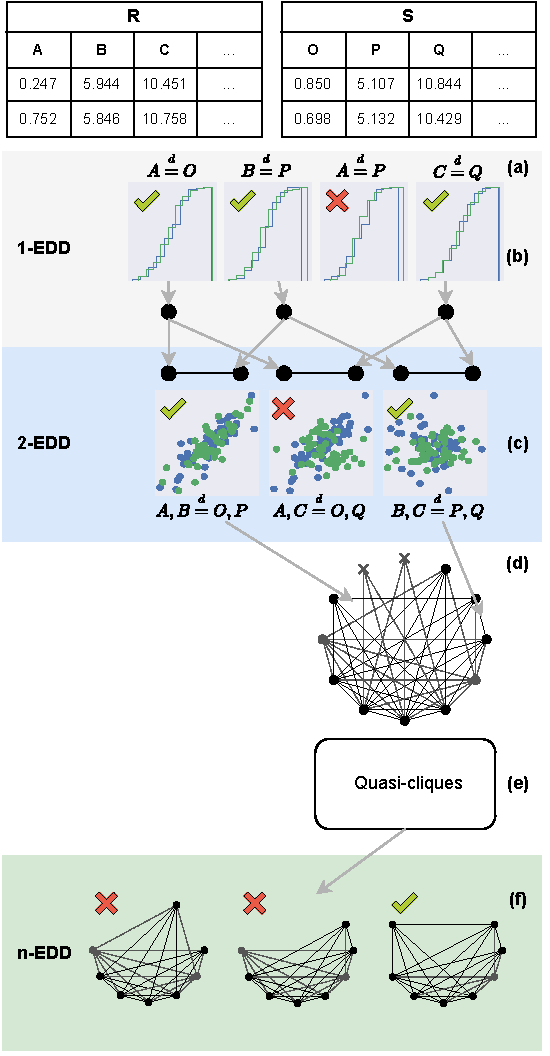
\includegraphics[width=\linewidth]{images/5_presq/pipeline}
    \caption{Simplified schematic of \PresQ.}
    \label{fig:presq_pipeline}
\end{figure}

 Given datasets $R$ and $S$,

(a) Candidate $1$-\glspl{EDD} are found applying the interval-tree as described in section~\ref{sec:presq_unary}.

(b) Those for which the Kolmogorov-Smirnov finds a significant difference are discarded,
    and the rest are mapped to nodes.

(c) All pairwise combinations are tested, and those equally distributed are
    (d) mapped to edges on a 2-hypergraph. The algorithm works with hypergraphs of any rank
    (e.g., triplets mapped to edges on a 3-hypergraph).
    
(e) \PresQ searches for quasi-cliques as described in section~\ref{sec:presq}.

(f) A quasi-clique of cardinality $n$ corresponds to an $n$-EDD, which is then validated by
a statistical test. Those rejected are decomposed to generate the edges for a 3-hypergraph, which are
verified (c), used to build a $3$-hypergraph (d) and finally passed as input back to (e).

The graph above displays spurious nodes and edges (light grey, dotted) and false negatives
(missing edges between dark nodes) based on attribute names. The full graph is not a valid
quasi-clique because the hypergeometric
test on the node degree (eq.~\ref{eq:deg_hyperclique_hypergeom}) prunes the two nodes shown with
crosses.
Three candidates of arity 8 are generated given the constrain on the number of edges 
(eq.~\ref{eq:edge_hyperclique}). Two of them are rejected by the $n$-dimensional statistical test and used to compute the edges of the $3$-hypergraph.

\end{multicols}
    
\newpage

\subsubsection{Parameters}

Before explaining how to tailor the parameterization of the quasi-clique finding for the purpose
of searching \glspl{EDD}, we need to remind that, given two sets of attributes $R[X]$ and $S[Y]$,
our algorithm builds on the null hypothesis $H_0: P(R[X]) = P(S[Y])$.
In other words, it is based on the \emph{assumption} that any \gls{EDD} candidate is valid.

Let $\alpha$ be the significance level chosen by the user before running the algorithm.
Let $G$ be the initial $k$-uniform hypergraph and let $K$ be a quasi-clique candidate.
Under $H_0$, $K$ represents a $|K|$-ary EDD, and by the projection rule,
all possible edges between the nodes in $K$ are also valid $k$-ary \glspl{EDD}.
If we run null hypothesis tests over these $k$-ary specialized \glspl{EDD},
by the definition of type-I error, we can expect as many as $\alpha \times \binom{|K|}{k}$ false rejections.
In other words, under $H_0$, we can expect a ratio of $\alpha$ missing edges.
This is equivalent to setting the threshold for equation~\ref{eq:edge_hyperclique} as:

\begin{equation*}
    \gamma = 1 - \alpha   
\end{equation*}

Adjusting $\lambda$ is less straightforward: a high threshold
will reject good candidates. A low one will accept spurious ones, triggering
unnecessary tests. Even worse, the spurious quasi-cliques tend to have a high cardinality.
Once rejected, they will cascade and cause an increase on lower-arity \glspl{EDD}
to be tested as much as $\binom{n}{k+1}$, where $n$ is the arity of the \gls{EDD} candidate,
and $k$ is the current level of the bottom-up exploration.

To solve this dilemma, we propose to use an adaptive value for $\lambda$ based on the
quasi-clique being checked: under $H_0$, there is no reason to think that any
particular subset of the edges from the clique has a higher probability of
having missing members. In other words, if a given node has an
unexpected low degree, it is most likely connected by spurious edges.

Let $N$ be the number of edges and $n$ the
maximum degree of the nodes on a clique with $|V'|$ nodes. Under this null hypothesis,
the degree of the nodes should roughly follow a hypergeometric distribution:
\begin{equation}
    \Pr(\operatorname{Degree}(v) = d)  = \frac{\binom{|E'|}{d} \binom{N - |E'|}{n - d}}{\binom{N}{n}}, \textrm{ for } v \in V'
    \label{eq:hypergeometric}
\end{equation}
This fact allows us to perform a statistical test and accept or reject our
quasi-clique candidate with a given significance level.
Figure~\ref{fig:hypergeom_sf} shows some examples of this distribution for a
quasi-clique with 29 nodes and the critical value for
a one-tail test with $\alpha = 0.05$. In other words, if the degree of a
node within a quasi-clique candidate is less than the critical value, we can reject the
null hypothesis and accept that the set of edges connecting the node are spurious.

\begin{figure}[ht]
    \centering
    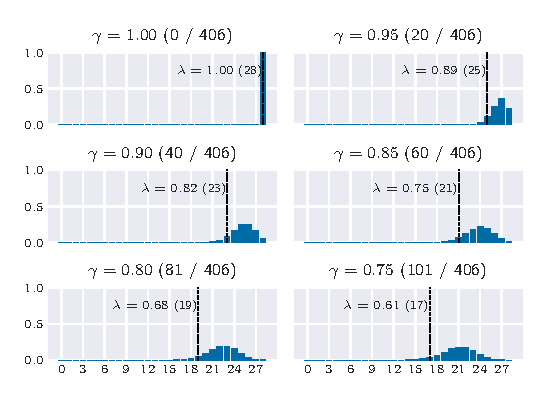
\includegraphics{images/5_presq/hypergeom}
    \caption[Distribution of the degree of the nodes under the assumption that missing edges
    are due to the expected false negative rate.]{
    Distribution of the degree of the nodes under the null hypothesis that the 
    missing edges on the quasi-clique are due to the expected false negative rate of the
    statistical test.
    The vertical line corresponds to the one-tail test with $\alpha = 0.05$.}
    \label{fig:hypergeom_sf}
\end{figure}

In summary, as a constant number of missing edges could be considered
too restrictive \cite{brunato2007effectively}, we consider a fixed ratio to be
limiting as well, and harder to make sense of ---i.e., why choose $\lambda = 0.6$
and not $\lambda = 0.7$?.
We propose that instead, replacing equation~\ref{eq:deg_hyperclique}
with equation~\ref{eq:deg_hyperclique_hypergeom} could be a more intuitive and
flexible approach.
\begin{equation}
    \forall v \in V': \operatorname{CDF}(\operatorname{Degree}(v)) \ge \Lambda
    \label{eq:deg_hyperclique_hypergeom}
\end{equation}
Where $0 \le \Lambda \le 1$. As with $\gamma$ and $\lambda$, a value of 1 would only accept
regular cliques.

The proposed parameterization for $\gamma$ and $\Lambda$ are internally consistent
since they are both constructed under $H_0$.

Figure~\ref{fig:presq_pipeline} visually summarizes the stages of \PresQ algorithm,
and the effects of the parameters $\gamma$ and $\Lambda$ on the quasi-clique finding stage.

In the following section, we will show that adapting \Find clique validation with ours
is enough to improve its performance in run-time and results. The \emph{growing}
step improves the efficacy (i.e. more maximal \glspl{EDD} found) at the cost of a higher run-time.

\section{Experiments}
\label{sec:presq_experiments}
We have implemented in Python a version of \Find that validates candidates with statistical
tests, and the proposed \PresQ.
Both share most of the code, including initialization and statistical
tests. Any difference in run-time is only because the modified version
searches for quasi-cliques instead of full cliques.

We focus on comparing these algorithms for two main reasons:
1) To prove that quasi-clique finding can outperform clique finding both in run-time and
results when the data is noisy, an advantage not necessarily exclusive to \gls{EDD} finding;
2) While \glspl{IND} are targeted towards inferring foreign-key relationships and generally of low arity,
we expect \glspl{EDD} to be of high arity ---\emph{co-located within a multidimensional space}---,
and \Find performs well when the arity is high~\cite{Dursch2019}.

\subsection{Experimental design}
\label{sec:experiment_design}
We have performed two different sets of experiments: one exclusively benchmarks the
quasi-clique search, while the other runs over real-world datasets.

\subsubsection{(Quasi-) clique search}
This experiment decouples the testing of the quasi-clique search from the uncertainty
associated with the data. The test accepts as parameters the rank
for the hyper-graph $k$, the cardinality for the clique $n$, the number of additional
nodes $N$, the fraction of missing edges $\alpha$ and the fraction of \emph{spurious}
edges $\beta$.
With these parameters, the test performs the following initialization procedure:

\begin{enumerate}
    \item Create $n$ nodes belonging to the clique
    \item Create $N$ additional nodes
    \item Create the set $E$ of $\binom{n + N}{k}$ edges connecting \emph{all nodes}
    \item Create the set $Q$ of $\binom{n}{k}$ edges belonging to the clique
    \item Obtain the set of all edges not belonging to the clique $C = E \setminus Q$
\end{enumerate}

With these sets, and to obtain an estimation of the distribution of the target measurement,
it then repeatedly generates noisy versions of the original clique through the following steps:

\begin{enumerate}
    \setcounter{enumi}{5}
    \item Remove $\alpha \times |Q|$ random edges from the original full clique $Q$
    \item Add $\beta \times |C|$ random edges from $C$
    \item Run \Find and \PresQ over the resulting graph
\end{enumerate}

The parameters $\alpha$ and $\beta$ simulate the effect of type I and type II errors
respectively.

\PresQ is configured with $\gamma = 1 - \alpha$ and $\Lambda = 0.05$. The number of additional nodes
is fixed to half the number of nodes in the clique: $N = \frac{n}{2}$.

This experiment measures, in a controlled manner, the capability of the
algorithms to find the \emph{true} clique and how their run-time is affected by the number of
missing and spurious edges.
Since the inputs are randomized, some will unavoidably run with exponential complexity,
the worst case for all the algorithms. To avoid spending too much time on these extreme cases,
the test also accepts a timeout parameter.
We describe the measurements we have taken in table \ref{tab:quasi_measurements}, and
the different parametrizations in table \ref{tab:quasi_params}.

\begin{table}[tbp]
    \caption{Set of measurements taken for the quasi-clique finding problem.}
    \label{tab:quasi_measurements}
    \centering
    \begin{tabular}{p{0.23\linewidth} p{0.7\linewidth}}
        \emph{Recovery ratio} & For each quasi-clique $Q'$ found, we compute the
        Jaccard index for each found quasi-clique,
        $J(Q, Q') = {|Q \cap Q'| \div |Q \cup Q'|}$.
        From all the obtained values, we report the maximum. A value of
        $1$ signals a perfect match. \\
        \emph{Time}           & Wall-clock time. \\
        \emph{Timeouts}       & How many runs exceeded the timeout. \\
    \end{tabular}
\end{table}

\begin{table}[tbp]
    \caption{Combination of parameters for the quasi-clique find problem.}
    \label{tab:quasi_params}
    \centering
    \begin{tabular}{c c c c r}
    \thead{Rank} & \thead{$\alpha$} & \thead{$\beta$} & \thead{Timeout (s)} \\
    \multirow{2}{*}{$2$} & $[0.05, 0.30]$, step $0.05$ & $0.0$ & \multirow{2}{*}{$240$} \\
    & $0.1$ & $[0.0 - 0.8]$ step 0.2 & \\[0.5cm]
    
    \multirow{2}{*}{$3$} & $[0.05, 0.30]$, step $0.05$ & $0.0$ & $300$ \\
    & $0.1$ & $[0.0 - 0.8]$ step 0.2 & $1200$ \\[0.5cm]
    
    \multirow{2}{*}{$4$} & $[0.05, 0.30]$, step $0.05$ & $0.0$ & $1200$ \\
    & $0.1$ & $[0.0 - 0.8]$ step 0.2 & $3000$ \\
    \end{tabular}
\end{table}

\subsubsection{Real-world datasets}
For the statistical tests, we use a non-parametric multivariate test based on
\gls{kNN}~\cite{Henze1988,Schilling1986b}, but any other multivariate
test could be used. However, regardless of the chosen test, there will always
be a number of false negatives bound by the significance level. In any case, the techniques
here discussed remain relevant.

The initialization stage of the test is as follows:

\begin{enumerate}
    \item We load two separate datasets.
    \item The constant columns, where every tuple has the same value ---including \emph{null}---
        or only a handful of different values, are dropped. \textsc{Faida} authors followed
        a similar procedure to reduce the number of columns to check \cite{Kruse2017}.
    \item A random sample is taken from both relations (it defaults to 200).
    \item The algorithm described in section~\ref{sec:presq_unary} is used to find a set of valid
        unary \glspl{EDD}.
    \item \emph{All} possible $n$-EDDs (for $n \in \{2, 3\}$) are generated and validated.
        The tests begin at different arities in order to compare the resiliency of
        \Find and \PresQ for different initial conditions.
    \item Valid $n$-EDDs are used to create the initial graph passed as input to \PresQ.
\end{enumerate}

The fifth step is performed at different significance levels of
$\alpha \in \{0.05, 0.10, 0.15\}$
to verify how the number of missing and spurious edges affects the search algorithms.
Typically, \Mind would generate the graph (i.e. 3-EDDs are generated from valid 2-EDDs).
Nonetheless, we start with all possible $n$-EDDs for simplicity: it is easier to
model and understand how many missing edges are expected as a function of $\alpha$.

The input for both search algorithms is, thus, identical at every run. However, since
there is an unavoidable effect of the randomization of the sampling in step 3 and the
$N$-dimensional permutation tests, we have repeated the experiment.
As a result, we are confident that the difference is significant and not due to chance.

While \Find has no parameters beyond the initial set of \glspl{EDD},
\PresQ requires a value for both $\gamma$ and $\Lambda$. As we mentioned earlier,
it makes sense to bind $\gamma$ to the expected number of missing edges
(false negatives): $\gamma = 1 - \alpha$. For $\Lambda$, we have tested with the
values 0.05 and 0.1 since lower values yield too many accidental quasi-cliques,
while higher values defeat the tolerance introduced by $\gamma$.

To measure the efficacy (\glspl{EDD} finding) and efficiency (run-time) of the algorithms,
we took the measurements summarized in tables \ref{tab:raw_measurements}
and \ref{tab:derived_measurements}.

\begin{table}[tbp]
    \caption{Set of measurements taken from individual runs.}
    \label{tab:raw_measurements}
    \centering
    \begin{tabular}{p{0.28\linewidth} p{0.63\linewidth}}
        \emph{Time}  & Wall-clock time, without accounting for the initialization stage,
                       as this is shared. \\
        \emph{Number of tests} & Time spent looking for quasi-cliques and validating the
                                   candidates.
                                   Tests can be potentially expensive, so we measure how many
                                   statistical tests are necessary. \\
        \emph{EDD count} & Without removing non-maximal \glspl{EDD}. \\
        \emph{Maximal EDD count} & Removing non-maximal \glspl{EDD}. \\
        \emph{Timeouts} & The execution time has a time limit of 3000 seconds. We report the
         percentage of runs that could not finish within the allocated time window. \\
        \emph{Highest arity} & The maximum \gls{EDD} arity found. \\
    \end{tabular}
\end{table}

\begin{table}[ht]
    \caption{Set of measurements derived over the complete set of runs.}
    \label{tab:derived_measurements}
    \centering
    \begin{tabular}{p{0.16\linewidth} p{0.75\linewidth}}
        \emph{Match ratio} & It is a ratio between the maximum arity of the maximal
        quasi-clique found and the \textit{true} maximum \gls{EDD} possible to find on
        each separate run.
        This \emph{truth} is solely based on attribute names. The algorithms can
        find higher arity \glspl{EDD} when the values are taken into account.
        This is a proof of success: the metadata would not have sufficed to capture
        this trait. \\
        
        \emph{Accuracy} & Measured as the number of total returned \glspl{EDD}, divided by
        the number of statistical tests executed. A ratio of $1$ (best) means that every
        candidate was accepted by the statistical test, while a ratio of $0$ (worst)
        means that all candidate quasi-cliques were rejected. This value is
        also affected by the power of the statistical test as a function of
        dimensionality.\\
    \end{tabular}
\end{table}

Given the variability and the number of dimensions, it can be hard to assess the quality
of the results. As a general guideline, we consider:

\begin{itemize}
    \item The higher the match ratio, the better: the highest arity EDD
    is potentially the most interesting and selective candidate for cross-matching.
    \item For a similar match ratio, the lower the run-time, the better.
\end{itemize}

For a similar match ratio, a higher number of maximal \glspl{EDD} is desirable. Arguably not
for the \gls{IND} discovery ---after all, a few good candidates may suffice---,
but it proves the capacity of finding maximal quasi-cliques.

It is important to note that some of these measures are interdependent. For instance,
if a maximal \gls{EDD} with a higher arity is found, the number of \glspl{EDD} should generally decrease.
Conversely, if a true, high arity candidate is rejected, multiple generalizations will be considered
and possibly accepted, increasing the number of unique \glspl{EDD}.
Similarly, finding more maximal \glspl{EDD} implies running more statistical
tests, so the run-time will be worse. Ultimately, it is up to the user to decide what is
more important and parameterize the algorithm accordingly.

We have run the tests disabling the limitation on the degree ($\Lambda = 0$) and
the limitation on the total number of edges ($\gamma = 0$). In this manner, we can
evaluate if there is any difference when using one, the other, or both.

\begin{table}[ht]
    \caption{Summary of the datasets used for validation.}
    \label{tab:dataset_summary}
    \centering
    \begin{tabular}{l c c r r}
        \textbf{Dataset}   & \textbf{Tables} & \textbf{Rows} & \textbf{Columns} & \textbf{1-EDD} \\
        Mortgage/Treasury  & 2               &   1k + 1k   & 16 + 16 &  26 \\
        Ailerons/Elevators & 2               &  14k + 17k  & 41 + 19 &  44  \\
        DC2                & 2               & 198k + 193k & 39 + 33 & 279 \\
        AFDS               & 4               & $172 \times 4$ & $8 \times 4$ & 63 \\
        Waveform           & 2               & 5k + 5k     & 22 + 41 & 145 \\
        KEEL      & 43              & 43 --- 41k  & 444 & 972 \\
        ChEMBLDB           & 79              & 5 --- 19M   & 418 & 599 \\
    \end{tabular}
\end{table}

\textbf{Datasets:} To test the algorithms, we have run them over two pairs of relations from the KEEL
regression datasets \cite{alcala2011keel}, the training and test catalog from the
\textit{Euclid photometric-redshift challenge} \cite{EuclidDesprez2020},
and a set of sensor measurements from an aircraft fuel distribution
system \cite{Gheraibia2019}. For the scalability tests, we have used the full
KEEL regression dataset, two variants from the Waveform Database
Generator~\cite{Dua:2019,breiman_classification_1984},
and versions 29 and 30 of the ChEMBL database~\cite{gaulton_chembl_2016}.

Some statistics about these datasets are summarized in table~\ref{tab:dataset_summary}.

\emph{Mortgage / Treasury} contain the same data, permuted by rows and by columns.
These datasets are an example of data de-duplication.

\emph{Ailerons /Elevators} share their origin (control of an F16 aircraft)
but have different sets of attributes. These datasets are an example of data fusion.

\emph{DC2} comes from a single catalog of astronomical
    objects, split based on the sky coordinates.
    The authors masked some of the attributes of the training set (i.e., coordinates and the
    target attributes: red-shift). 
    Therefore, both catalogs share some of the attributes but for different sources.
    A naive one-to-one schema matching will
    easily mistake these attributes for small sample sizes. In contrast, for bigger samples
    some true correspondences will be falsely rejected.
    These datasets require some more resilient methods capable of working on a
    multidimensional space.
    These datasets are an example of schema inference/matching and automatic feature discovery.
    
\emph{\gls{AFDS}} comprises five different files,
    all sharing the same schema but containing sensor measurement values for different scenarios:
    one nominal, and four abnormal. Our implementations of \Find and \PresQ can process
    the five files at the same time.

\emph{Waveform Database Generator}
    We use version 1, with 21 attributes, and version 2, which shares the same 21 attributes and adds 19
    extra features that are just Gaussian noise. This 21-ary \gls{EDD} between the datasets goes
    beyond the maximum 7-ary evaluated in previous works~\cite{Dursch2019}.
    Additionally, the number of attributes and their distribution similarity generates many false positives at low
    dimensionality, stressing the capability of processing noisy, dense, graphs.

\emph{ChEMBL Database}
    We use versions 29 and 30 of the ChEMBL database, each of size 20GiB. They are
    stored on \textsc{BeeGFS}, a clustered filesystem. We evaluate the scalability with respect to the number of
    columns, adding tables progressively. In this scenario, the overhead introduced by the sampling becomes significant.

The two pairs from KEEL (i.e. Mortgage/Treasury and Ailerons/Elevators) were found
running over the whole KEEL dataset initial versions of the algorithms described in
this paper, proving their capabilities. We report the performance of this exercise, together
with the other two scalability tests, in section \ref{sec:scalability}.

\subsection{Environment}

The tests were run on a cluster, where each node
is fitted with an Intel(R) Xeon(R) Gold 6240 CPU at 2.60GHz with 36 virtual cores,
running on a standard CentOS Linux 7.9. The default memory allocation per core was
3 GB. 

For the (quasi-)clique search, we submitted one job with as many tasks as
parameter combinations described in table \ref{tab:quasi_params} and 1 CPU per task,
for cliques of size $10, 20$ and $30$.  We chose the time limit based on the measured
run-time from early test runs.

For the real dataset tests, we submitted jobs with 8 tasks and 1 CPU per task,
limited to 24 hours. The objective of concurrent runs was to increase the number
of data points since the code has not been parallelized.

Finally, we executed ten randomized runs for each increment on the number of columns for the scalability tests.

\subsection{Results}
\label{sec:results}

In this section, we will summarize the results from our test setup.

\subsubsection{(Quasi-) clique search}
\label{sec:result_quasi_search}

We summarize the \emph{wall-time} and \emph{recovery ratio} metrics by estimating
their distribution mean and its associated standard error following the Bootstrap method.
The \emph{timeout} is measured by counting how many runs fail to find a quasi-clique within
the allocated time window.

While the \emph{wall-time} distribution is far from Gaussian, we consider that randomizing the
input, pruning the long-running cases, and averaging the results of a few short-running
iterations is a valid usage of the algorithms. This makes comparing the means a reasonable
assessment.

\textbf{Influence of spurious edges:}
We show in figure~\ref{fig:3hyper_beta} the performance of the algorithms for $3$-hypergraphs
and different ratio of spurious edges. The exponential worst-case
complexity becomes more apparent the more connected nodes there are.
\Find is the most affected, but at some point, \PresQ performance also degrades significantly and eventually also fails to finish on time.
These results confirm that spurious edges influence the
\emph{run-time} of these algorithms very negatively~\cite{koeller2006heuristic}.

\begin{figure}[ht]
    \centering
    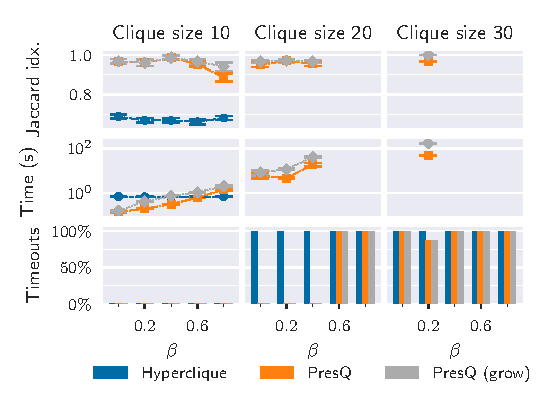
\includegraphics{images/5_presq/3hyper_beta}
    \caption[Recovery ratio and run-times for cliques on uniform $3$-hypergraphs for different ratios of spurious edges.]{
        Recovery ratio and run-times for cliques on uniform $3$-hypergraphs
        for different ratios of spurious edges ($\beta$).
        Each data-point corresponds to 15 runs.
    }
    \label{fig:3hyper_beta}
\end{figure}

\textbf{Influence of missing edges:}
Figure~\ref{fig:3hyper_alpha} shows that our proposal
generalizes for hypergraphs. \PresQ with the growing stage enabled, oscillates very close
to the original clique even when $30\%$ of the edges are missing. However, the number of
timeouts increases given that the algorithm needs to traverse more levels from the seed to the maximal
quasi-clique. Interestingly, there is an inverse correlation between the number
of missing edges and run-time.

\begin{figure}[ht]
    \centering
    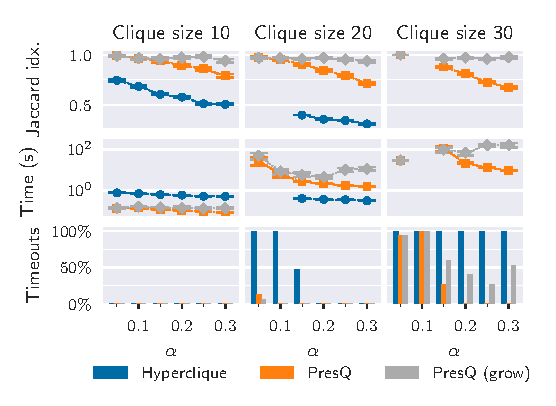
\includegraphics{images/5_presq/3hyper_alpha}
    \caption[Recovery ratio and run-times for cliques on uniform $3$-hypergraphs
    for different ratios of missing edges.]{Recovery ratio and run-times for cliques on uniform $3$-hypergraphs
    for different ratios of missing edges ($\alpha$).
    Each data-point corresponds to 15 runs.}
    \label{fig:3hyper_alpha}
\end{figure}

\textbf{Influence of correlated ratios:}
In a more realistic scenario --- i.e., when using statistical tests --- as the number of missing edges
increases, the number of spurious edges should decrease.
We have run tests with the growing stage enabled for different parametrization on the node degree
threshold. This includes a regular $\lambda$ parameter with a value of $0.8$ chosen based on
good empirical results we obtained during early iterations of this work.
The correlation between $\beta$ and $\alpha$ is based on the empirical statistical power of the
kNN test as a location test on $k$ dimensions and a sample size of 100.
In all cases, $\gamma = 1 - \alpha$.

Figure~\ref{fig:hyper_ab_corr} summarizes the results. A hand-picked parameter of $\lambda = 0.8$ can
perform well for some hypergraphs but quickly underperforms as the hypergraphs become noisier.
To the contrary, our proposal based on the hypergeometric distribution remains stable.
However, disabling the degree limitation performs better for this particular setup.
This makes sense since there is no correlation between missing edges.

\begin{figure}[ht]
    \centering
    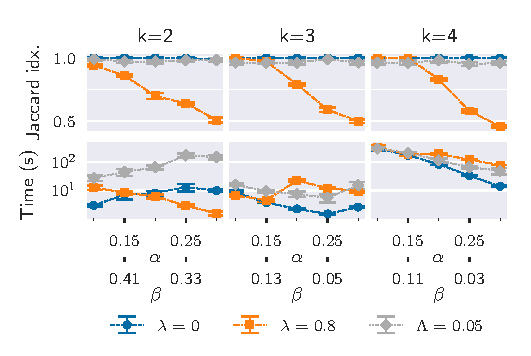
\includegraphics{images/5_presq/quasi_corr_20}
    \caption[Recovery ratio and run-times for cliques of size 20 on uniform $(2,3,4)$-hypergraphs.]{
    Recovery ratio and run-times for cliques of size 20 on uniform $(2,3,4)$-hypergraphs.
    In this setup there were no timeouts. Each data-point corresponds to 5 runs.
    }
    \label{fig:hyper_ab_corr}
\end{figure}

\subsubsection{Real-world datasets}
\label{sec:results_real}

The initial randomized state heavily influences the proposed performance measurements.
Their distribution can not be assumed normal.
Purely comparing their means is not enough to assess the validity of our proposal, and we also need an estimation of variability.

The metric of choice used to compare our measurements is the \emph{percent difference}
between sample means, being its sample estimator~\cite{campelo_sample_2019}:

\begin{equation}
    \label{eq:percent_difference}
    \hat{\phi} = \frac{\hat{\mu}_{\PresQ} - \hat{\mu}_{\Find}}{\hat{\mu}_{\Find}}
\end{equation}

The distribution of
$\hat{\phi}$ can be estimated using bootstrapping.
In this manner, we obtain the estimated population mean and standard deviation. Finally,
we compute the $95\%$ confidence interval $\hat{\mu_\phi} \pm 1.96 \hat{\sigma_\phi}$

Figure \ref{fig:results_summary} shows this confidence interval for match ratio, unique \glspl{EDD},
number of tests and wall time (columns) for a significance level of $0.10$, against the
different datasets (rows).

The DC2 case is particularly interesting. The attributes of the datasets
are relatively numerous ---compared to the others--- and very similar in their distributions.
A low initial significance level will generate very dense graphs, with a few missing edges, and
many spurious, which impacts the performance considerably.
This is a known issue of \Find~\cite{koeller2006heuristic}.
Increasing the significance level reduces the number of spurious edges, at the cost of
missing true ones. Consequently, the efficiency is improved at the cost of the efficacy.
\PresQ allows us to increase the significance
level without sacrificing much efficacy.

For the \gls{AFDS} dataset, when comparing the maximum \gls{EDD} arity found per pair of files,
scenarios two and three are the most similar, as seen in figure~\ref{fig:afds}.
We can obtain this insight without even knowing what the schema nor the content of the files are.
After seeing this result, we checked the original paper from
where the dataset was obtained, verifying that, indeed, they are
``two closely related scenarios'' \cite{Gheraibia2019}.
We consider this another proof of the utility of the proposed techniques.

\begin{figure}[ht]
    \centering
    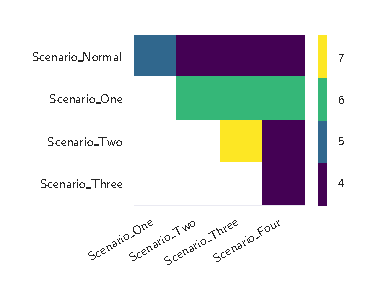
\includegraphics[width=0.5\linewidth]{images/5_presq/afds}
    \caption{
        Pairwise max arity found on the \glsfmtshort{AFDS} dataset for each pair of scenarios
    }
    \label{fig:afds}
\end{figure}

Table~\ref{tab:ind2_summary} summarizes the overall results when
we execute our tests over the datasets \emph{Mortage vs Treasury},
\emph{Ailerons vs Elevators} and \emph{DC2} for different values of $\gamma$ and $\Lambda$ ---
note that \Find is equivalent to either one of the two parameters set to $1.$. For run-time,
match ratio, and the number of unique \glspl{EDD}, we provide the first and third quartiles.
The \emph{precision} column shows a measure of how many candidates are accepted by the
statistical test. A value of $1$ means that all candidates were valid \glspl{EDD}.

When the search algorithm looks for cliques (the first entry for each dataset),
the precision is high since almost all candidates were accepted. However,
these candidates are, on average, of lower arity. This is visible on the \emph{Match}
columns. As the potential maximal arity becomes higher ---e.g., \emph{DC2}--- the
chance of having missing edges increases, thus making the search more resource intensive.

On the other hand, in a too permissive setup where only $\gamma$ constrains the quasi-cliques
(second entry), the algorithm is too eager and accepts \gls{EDD} candidates later rejected either
by the statistical test or by the limitation of not accepting duplicated columns.
The precision is low, and the search time increases as well.

Our proposed $\Lambda$ parameter, based on the \emph{expectation} on the number of missing edges,
is more effective at constraining the set of candidates even when used alone (third entry).
The precision increases and the run-time is reduced.
When combined with $\gamma$ (fourth and fifth entries), the precision increases, and fewer
tests are required.

As an illustration of this balance, let us examine in more detail the consequences of the
different $\Lambda$ parameterization following the process shown in figure~\ref{fig:presq_pipeline}
when running over the DC2 dataset. The first four stages are unaffected by this parameter:

\begin{enumerate}[label=({\alph*}),align=parleft,leftmargin=!,labelwidth=1em]
\item As described in section~\ref{sec:presq_unary}, an interval tree is built over the attributes
    from both relations. Only overlapping ranges are compared,
    reducing by $~27\%$ the number of tests required.
\item $~810$ KS tests need to be done. $~49$ pairwise combinations are considered equally distributed
    (\glspl{uEDD}).
\item $(n \times (n - 1)) \div 2 ~= 1176$ edges are build combining all \glspl{uEDD} and validated
    using the \gls{kNN} test. $~612$ edges are considered valid.
\item The initial graph has half as many edges as the complete graph.
    Since we know the ground truth, we can extract the sub-graph induced by the set of
    true \gls{uEDD} and find the number of missing edges to be $\approx 0.10$ on average,
    as we expected.
\end{enumerate}

\medskip

The following table exemplifies the consequences of different values of $\Lambda$
--- see equation~\ref{eq:deg_hyperclique_hypergeom} --- on
the count and size of the found quasi-cliques (e) and the number validated by the \gls{kNN} test (f).
Those invalid are `decomposed' into candidate $3$-EDDs, validated, and 
used to build a $3$-hypergraph (d) feedback to the stage (e) for the next iteration.

\begin{tabular}{lrrr}
                   & \thead{Quasicliques} & \thead{Valid} & \thead{Median size} \\
$\Lambda = 0.00$   & 2385                 & 292       & 19        \\
$\Lambda = 0.05$   & 107                  & 64        & 12        \\
$\Lambda = 1.00$\footnotemark   & 53053   & 52291     &  6         \\
\end{tabular}

\footnotetext{Equivalent to clique finding}

\medskip

For $\Lambda = 0$, the search algorithm is too greedy and accepts quasi-cliques that are poor candidates.
Too many are invalid and need to be feedback to the algorithm, increasing run-time.
For $\Lambda = 1$, the search algorithm is too restrictive. Its precision is high,
but it spends much time enumerating small cliques. $\Lambda = 0.05$ provides the right balance,
improving the result and performance.

Finally, the growing stage increases the number of candidates of all arities.
This requires a more exhaustive traversal of the search space and the execution of more tests,
increasing the total run-time. While we run the growing stage over
\emph{all} found seeds this stage could be restricted only
to a subset of the most interesting \emph{seeds} ---e.g., highest cardinality.

\begin{figure*}[t]
    \centering
    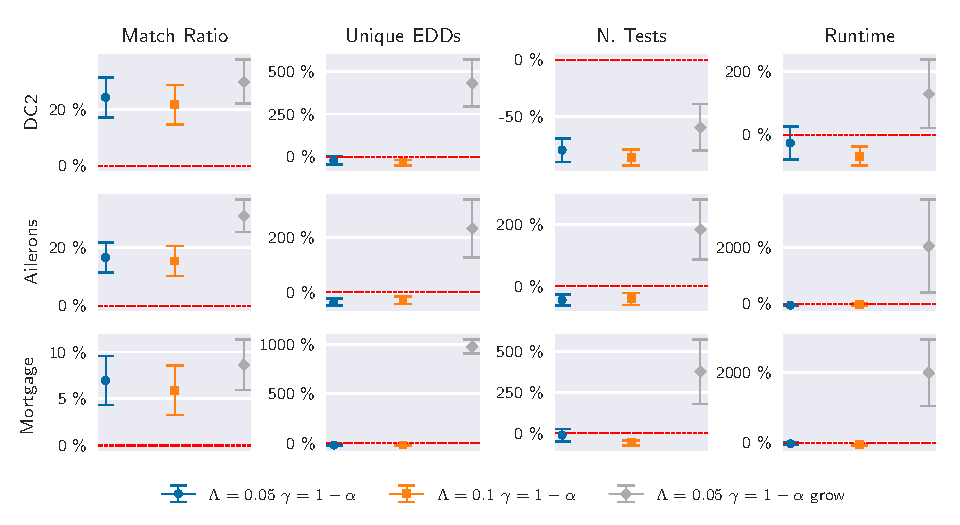
\includegraphics[width=\linewidth]{images/5_presq/all}
    \caption[$95\%$ confidence intervals for the percent difference between \Find and \PresQ.]{
        $95\%$ confidence intervals for the percent difference
        (equation \ref{eq:percent_difference}) between \Find and
        three parameterizations of \PresQ for the DC2, Ailerons vs. Elevator, and
        Mortgage vs. Treasury datasets.
        Intervals that do not intersect the horizontal dashed line at $0\%$  show a statistically
        significant result.
        For ratio, higher is better. For tests and run-time, lower is better. Unique is harder to
        assess since the results also depend on the statistical power of the chosen test.
        Since the growing stage can generate many candidates, a low-powered test will accept
        many false \glspl{EDD}.
    }
    \label{fig:results_summary}
\end{figure*}

% Results starting arity 2
\begin{table*}[htb]
    \caption[Summary of run-time, matching ratio, and number of maximal quasi-cliques found.]{
        Summary of run-time, matching ratio (based on name), and number of maximal quasi-cliques found
        accepted by the statistical test.
        The significance level is $\alpha = 0.1$.
        $N$ corresponds to the number of randomized runs.
        \PresQG identifies \PresQ with the growing stage.
    }
    \label{tab:ind2_summary}
    \centering
    \resizebox{\textwidth}{!}{%
    \begin{tabular}{l r r | r r | r r | r r | r | r | r}
    
    \multicolumn{11}{c}{\textit{Mortgage vs Treasury}} \\
    
    & \thead{$\Lambda$} & \thead{$\gamma$} & \multicolumn{2}{c|}{\thead{Time (s)}} &
        \multicolumn{2}{c|}{\thead{Match}} & \multicolumn{2}{c|}{\thead{Unique}} &
        {\thead{Prec.}} & {\thead{N}} & \thead{Timeouts} \\

    & & & \textit{Q1} & \textit{Q3} & \textit{Q1} & \textit{Q3} & \textit{Q1} & \textit{Q3} & \\ \hline
    
    \Find   &                &               &   0.44 &   0.64 & 0.75 &	1.00 &  12 &  21 & 0.99 & 527 & 0.0\% \\
    \PresQ  & \bfseries 0.00 &           0.9 &  44.86 & 459.04 & 0.94 & 1.00 &  11 &  15 & 0.06 & 212 & 0.0\% \\
    \PresQ  &           0.05 & \bfseries 0.0 &   0.71 &  11.08 & 0.88 & 1.00 &  11 &  17 & 0.49 & 535 & 0.0\% \\
    \PresQ  &           0.05 &           0.9 &   0.76 &  10.61 & 0.88 &	1.00 &  11 &  17 & 0.57 & 507 & 0.0\% \\
    \PresQ  &           0.10 &           0.9 &   0.73 &   1.99 & 0.84 & 1.00 &  11 &  17 & 0.75 & 503 & 0.0\% \\
    \PresQG &           0.05 &           0.9 &  47.10 &	247.39 & 0.88 &	1.00 & 125 & 262 & 0.22 & 503 & 0.0\%\\

    \\
    \multicolumn{11}{c}{\textit{Ailerons vs Elevators}} \\
    
    \Find   &                &               &  5.63 &  48.41 & 0.78 & 1.00 & 142 &	 291 & 0.98 &  93 & 0.0\% \\
    \PresQ  & \bfseries 0.00 &           0.9 &  8.82 &  36.75 & 1.00 & 1.22 &  88 &  174 & 0.24 & 128 & 0.0\% \\
    \PresQ  &           0.05 & \bfseries 0.0 & 22.68 &  52.87 & 1.00 & 1.22 & 113 &  239 & 0.16 & 126 & 0.0\% \\
    \PresQ  &           0.05 &           0.9 &  7.51 & 	20.12 &	1.00 & 1.11 &  86 &	 198 & 0.35 &  60 & 0.0\% \\
    \PresQ  &           0.10 &           0.9 &  6.83 & 	22.40 & 1.00 & 1.11 &  89 &	 205 & 0.41 &  60 & 0.0\% \\
    \PresQG &           0.05 &           0.9 & 57.86 & 674.26 &	1.11 & 1.25 & 321 &	1062 & 0.22 &  60 & 0.0\% \\
    
    \\
    \multicolumn{11}{c}{\textit{DC2}} \\
    
    \Find   &                &               &   74.94 &  805.71 & 0.60 & 0.71 &  73 & 150 & 0.90 &  53 & 34.0\% \\
    \PresQ  & \bfseries 0.00 &           0.9 &  681.51 & 1536.19 & 0.68 & 0.69 & 102 & 200 & 0.01 &  16 & 87.5\% \\
    \PresQ  &           0.05 & \bfseries 0.0 &  40.07 &   189.45 & 0.80 & 0.93 &  46 & 115 & 0.10 &  21 & 47.6\% \\
    \PresQ  &           0.05 &           0.9 &   25.57 &  214.27 & 0.76 & 0.89 &  46 & 113 & 0.14 &  53 & 13.2\% \\
    \PresQ  &           0.10 &           0.9 &   18.61 &  144.98 & 0.76 & 0.87 &  42 &  98 & 0.18 &  52 & 23.1\% \\
    \PresQG &           0.05 &           0.9 &  458.26 & 1881.02 & 0.81 & 0.93 & 518 & 798 & 0.23 &  52 & 50.0\% \\
    \end{tabular}}
\end{table*}

% Results starting at arity 3
\begin{table*}[htpb]
    \caption[Summary of run-time, matching ratio, and number of maximal quasi-cliques found with an initial arity $k = 3$.]{
        Summary of run-time, matching ratio (based on name), and number of maximal quasi-cliques found.
        Significance level is $\alpha = 0.1$, initial arity $k = 3$.
    }
    \label{tab:ind3_summary}
    \centering
    \small
    \resizebox{\textwidth}{!}{%
    \begin{tabular}{l r r | r r | r r | r r | r | r | r}
    
    \multicolumn{11}{c}{\textit{Mortgage vs Treasury}} \\
    
    & \thead{$\Lambda$} & \thead{$\gamma$} & \multicolumn{2}{c|}{\thead{Time (s)}} &
        \multicolumn{2}{c|}{\thead{Match}} & \multicolumn{2}{c|}{\thead{Unique}} &
        {\thead{Prec.}} & {\thead{N}} & \thead{Timeouts} \\
        
    & & & \textit{Q1} & \textit{Q3} & \textit{Q1} & \textit{Q3} & \textit{Q1} & \textit{Q3} & & \\ \hline
        
    \Find    &                &             &   8.75 &  20.54 & 0.75 & 1.00 &  86 & 144 & 1.00 & 160 & 16.3\% \\
    \PresQ   &  \textbf{0.00} &         0.9 &  55.00 & 569.01 & 1.00 & 1.00 &  67 & 102 & 0.17 & 160 &  0.0\% \\
    \PresQ   &           0.05 &         0.9 &   8.43 &  19.45 & 0.81 & 1.00 &  82 & 126 & 0.99 & 160 &  0.0\% \\
    \PresQ   &           0.10 &         0.9 &   9.04 &  19.60 & 0.81 & 1.00 &  83 & 130 & 0.99 & 160 &  0.0\% \\
    \PresQG  &  \textbf{0.00} &         0.9 &   6.71 & 902.57 & 0.87 & 1.00 &  98 & 264 & 0.29 & 160 & 47.5\% \\
    \PresQG  &           0.05 &         0.9 &  36.83 & 358.53 & 0.86 & 1.00 & 204 & 395 & 0.98 & 160 &  0.6\% \\
    \PresQG  &           0.10 &         0.9 &  43.23 & 287.59 & 0.81 & 1.00 & 198 & 376 & 0.98 & 160 &  0.0\% \\
        
    \\
    \multicolumn{11}{c}{\textit{Ailerons vs Elevators}} \\
    
    \Find    &                &               &  24.66 & 1072.74 & 0.89 & 1.00 & 474 &  947 & 1.00 & 114 & 40.4\% \\
    \PresQ   &   \textbf{0.00}&           0.9 &  28.55 &  140.93 & 1.13 & 1.33 & 276 &  627 & 0.45 & 114 &  1.8\% \\
    \PresQ   &           0.05 &           0.9 &  26.59 &   83.72 & 1.11 & 1.22 & 339 &  656 & 0.95 & 114 & 14.0\% \\
    \PresQ   &           0.10 &           0.9 &  25.55 &  105.93 & 1.00 & 1.14 & 357 &  680 & 0.96 & 110 & 14.6\% \\
    \PresQG  &  \textbf{0.00} &           0.9 & 171.81 &  940.15 & 1.19 & 1.33 & 498 & 1044 & 0.34 & 114 &  9.7\% \\
    \PresQG  &           0.05 &           0.9 & 174.88 &  670.84 & 1.13 & 1.29 & 629 & 1330 & 0.95 & 111 & 18.9\% \\
    \PresQG  &           0.10 &           0.9 & 205.63 &  718.51 & 1.12 & 1.29 & 661 & 1245 & 0.95 & 109 & 19.3\% \\

    \\
    \multicolumn{11}{c}{\textit{DC2}} \\
    
    \Find    &                &               & 1050.56 & 1050.56 & 1.00 & 1.00 & 560 & 560 & 0.97 & 83 &  98.8\% \\
    \PresQ   &  \textbf{0.00} &           0.9 &  599.20 &  599.20 & 0.88 & 0.88 & 830 & 830 & 0.06 & 32 &  96.9\% \\
    \PresQ   &           0.05 &           0.9 &  207.28 & 2013.45 & 0.81 & 0.89 & 351 & 747 & 0.56 & 81 &  88.9\% \\
    \PresQ   &           0.10 &           0.9 &   71.85 &  926.94 & 0.80 & 0.93 & 380 & 791 & 0.72 & 78 &  93.6\% \\
    \PresQG  &  \textbf{0.00} &           0.9 &         &         &      &      &     &     &      & 32 & 100.0\% \\
    \PresQG  &           0.05 &           0.9 &  340.72 &  599.10 & 1.02 & 1.21 & 775 & 888 & 1.00 & 80 &  97.5\% \\
    \PresQG  &           0.10 &           0.9 &  413.58 &  670.53 & 1.00 & 1.13 & 808 & 947 & 1.00 & 76 &  97.4\% \\
    \end{tabular}}
\end{table*}

Table~\ref{tab:ind3_summary} summarizes the performance measures when \Find and \PresQ are run over an initial
3-hypergraph. The precision is considerably higher than when starting on a 2-hypergraph.
This is due to the higher power of the statistical test at dimension 3, so fewer spurious edges are introduced.
However, the overall run-time suffers because the number of edges on an hypergraph is determined by the expression
$\binom{|V|}{k}$ where $|V|$ is the number of nodes and $k$ the rank of the hypergraph.
Therefore, for a fixed number of nodes, the number of edges is generally higher for hypergraphs of higher rank.

\subsubsection{Scalability tests}
\label{sec:scalability}

For measuring the scalability of our algorithm, we executed the algorithm over the KEEL, Waveform, and ChEMBL datasets, progressively adding columns, measuring run-time; the
number of $1$, $2$, and $n$-EDDs; and the number of unary tests saved by the interval
tree.
In all cases the chosen parameterization is $\alpha=0.1$, $\Lambda = 0.05$,
$\gamma = 1 - \alpha$ and 200 samples. We set the run-time limit at 3000 seconds.
The relations and their attributes are consistently added in alphanumeric order.
Figure~\ref{fig:scalability} summarizes our results.

The accepted $1$-EDDs are used to compute all the possible $2$-EDDs, while the accepted $2$-EDDs
define the initial edges for the $n$-EDD finding.


The \emph{KEEL} dataset contains 43 different relations. The interval tree saves around 45\% of
the tests since many columns do not overlap. The number of \glspl{EDD} increments in `bursts' when a
relation that matches a previous one enters the pool. This is due to the existence of
high arity \glspl{EDD} (16, 12, 7 and 6).
The high number of $2$-EDDs makes the growing stage eventually impractical.

For the \emph{ChEMBL} databases, we have used a naive random sampling that only requires a single
pass over the entire database. Even then, the reading time is small with respect to the rest of the EDD
finding algorithm. The number of $1$-EDDs steadily increments as relations are added, but $2$
and $n$-EDDs remain relatively stable ---the corresponding error bars overlap---, and so does the run-time.
The arities are lower than those from KEEL, the maximum being 6 for the tables \texttt{molecule\_dictionary}
and \texttt{compound\_properties}. The interval tree saves 57.9\% tests for 1-EDDs.

Finally, while the \emph{Waveform Generator} datasets are the smallest, it is the case for which the
algorithm shows the worst performance. This is due to the high arity possible (up to 20), and 
because the attributes are hard to distinguish ---the interval tree can not save even one test. The
number of $2$-EDDs grows super-linearly with respect to the number of attributes, resulting in a very
dense and noisy initial graph with many possible quasi-cliques.

From these experiments, we can conclude that the algorithm scales well in relation with the number of
relations and columns and that the sampling has a low impact even for big datasets.
However, when the statistical test has low power for the input data, the run-time significantly degrades even for moderate input sizes since the search space is combinatorial and little
pruning is possible. Then the user can choose a different test or increase the sample size to increase the
power. Figure~\ref{fig:scalability_sample_size} exemplifies the effect the sample size has on the result
set and, therefore, run-time for the complete Waveform dataset. The power of the test is low for low
dimensionality, and the initial graph becomes very dense.

\begin{figure*}[htb]
    \centering
    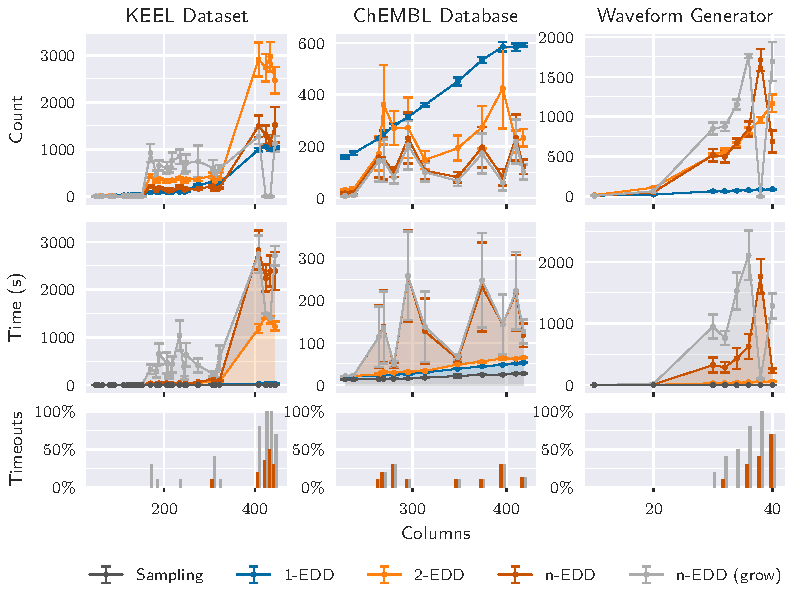
\includegraphics{images/5_presq/scalability}
    \caption[Scalability of \PresQ with respect to the number of columns.]{
        Scalability of \PresQ with respect to the number of columns.
        The top row corresponds to the number of \glspl{EDD} with arities 1, 2, and $n \ge 3$.
        The middle row shows the time spent on each stage: sampling, searching, and testing for the different arities.
        Note that the two n-EDDs variants are stacked over the previous stages, displaying the total run-time.
        The last row shows the percentage of runs timed out at 50 minutes.
        Each data-point summarizes between 10 and 13 randomized runs.
    }
    \label{fig:scalability}
\end{figure*}

\begin{figure}[htb]
    \centering
    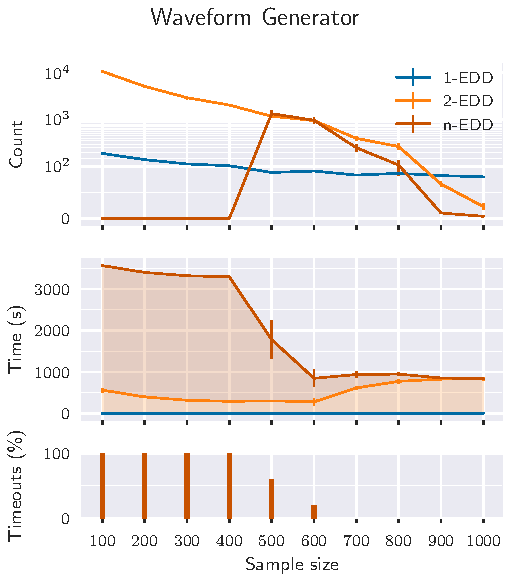
\includegraphics{images/5_presq/scalability_sample_wave}
    \caption[Scalability of \PresQ with respect to the number of samples.]{
        Scalability of \PresQ with respect to the number of samples for the Waveform datasets.
        Note that for the top row the $y$ axis is linear between $0$ and $100$, and
        logarithmic afterwards. Each data-point summarizes 10 randomized runs.
    }
    \label{fig:scalability_sample_size}
\end{figure}

\FloatBarrier

\section{Conclusions}
\label{sec:presq_conclusions}

Finding sets of equally-distributed dependencies between numerical datasets is a similar
problem to that of finding Inclusion Dependencies between tables in a relational model.
However, the statistical nature of tests, with their potential uncertainties, can make
their finding more complicated and considerably degrade the performance of existing algorithms.
This problem can be mapped to finding quasi-cliques, as the \gls{IND} problem can be
mapped to finding full cliques.

In this chapter, we have introduced the concept of EDD, similar to the \gls{IND} from
the relational domain. We have proposed \PresQ, a new algorithm based on the search of
maximal quasi-cliques on hyper-graphs. We have proven that by limiting the quasi-cliques
by the number of missing edges, and the degree of the nodes, our algorithm can successfully
identify shared sets of attributes.

In general, comprehensive approaches will be needed to find very high arity \glspl{EDD},
given the complexity of the \gls{IND}/\gls{EDD} discovery problem.
In chapter~\ref{chapter:conclusions} we discuss some possible directions for future research.

All the necessary code to reproduce our tests, our
measurements, and figures, are publicly available\footnote{\url{https://doi.org/10.5281/zenodo.6865856}}.


\chapter{Two-sample test based on \glsfmtlong{SOM}}
\label{chapter:som}
%I think it is a good idea to include this.
%"Bridge the gap between schema matching and perf.access". I like it.
% Borne, list of science requirements!! Justifies this.

\section{Introduction}

A classification task can be seen as a sort of two-sample statistical test.
If a classifier trained over two samples can effectively distinguish between
them with better-than-chance performance, the classifier rejects the null
hypothesis that both samples come from the same distribution~\cite{friedman2004multivariate}.

While a formal statistical test can be more suitable when the alternative
hypothesis is known, machine learning classifiers can be a good alternative
when the data is complex and abundant~\cite{kirchler2020two,kim2021classification,pmlr-v119-liu20m}.

Furthermore, the representation ``learned'' by some classifiers can be helpful
to examine how the samples differ~\cite{friedman2004multivariate,lopez2016revisiting},
or it could be used later for other purposes, such as directly classifying future samples.

\medskip

\gls{SOM} is a technique for dimensionality
reduction. It is a type of neural network that learns a low-dimension representation
- generally 2D - of the original high-dimensional space while maintaining the topological
layout of the original data~\cite{kohonen1982self, Villmann1999}.

The learned map can be directly used for unsupervised clustering --- when the map is big enough ---
and classification tasks if the training data is labeled~\cite{ultsch2005esom,ultsch2007emergence}.
For instance, the neurons can be labeled according to the training data labels mapped into their
region. During classification, objects can be labeled according to the label of the neuron
into which they are mapped.
Thus, \glspl{SOM} can be used as a building block of an ML-based two-sample test, similar to
\gls{kNN} or \emph{Neural Network} classifiers, with the valuable addition
of producing a representation that can be visualized.

In this chapter, we propose a multivariate statistical test based on
Self-Organizing Maps that shows performance comparable to other techniques based on 
machine learning models and even superior for medium to big sample sizes. In addition to the 
$p$ value for $H_0: P = Q$, the test also outputs a trained \gls{SOM} model that can be of
use for other tasks, such as classification or visualization.
Our proposal uses a $\chi^2$ statistic to compare the densities of both samples on
the projected plane instead of relying on a training-testing split. This allows us to fully
utilize the sample data. To our knowledge, using Self-Organizing Maps
to perform multidimensional two-sample testing has not been proposed
before~\cite{kaski1998bibliography,oja_bibliography_2003,polla_bibliography_2006}.

This statistical set can potentially be used with \PresQ to validate
high-dimensional \glspl{EDD}. The resulting projection can be used to identify objects
from multiple datasets that are co-located in the matched multidimensional space, satisfying
two of Borne's science requirements for data mining: \emph{Object Cross-Correlation} and
\emph{Nearest-neighbor identification}.

In section~\ref{sec:som_chi2}, we describe our proposal
for a multidimensional non-parametric statistical test based on Self-Organizing Maps.
In section~\ref{sec:som_definitions}, we introduce classifier two-sample tests
and \glsxtrlong{SOM}.
In section~\ref{sec:som_exp_setup}, we describe the experimental setup we have used
to validate our proposal --- including the parametrization of the existing techniques
evaluated as a baseline ---. In section~\ref{sec:som_results} we present the results.
Finally, in section~\ref{sec:som_conclusions}, we compile our conclusions and propose areas for future
work.


\section{Definitions}
\label{sec:som_definitions}

\paragraph{Classifier two-sample tests.}
\label{sec:som_classifier2sample}
A binary classifier can be seen as a two-sample test. If a classifier has a better-than-chance
performance, it can be inferred that the two classes do not originate from the same underlying
population~\cite{friedman2004multivariate}. 

More formally, given two sets, $X = \{x_0,x_1,\ldots,x_n\}$ sampled from $P$, and \linebreak
$Z = \{z_1,z_2,\ldots,z_m\}$ sampled from $Q$. A test statistic $\hat t \sim T$ is used to
``summarize'' the difference between both samples and, depending on a pre-established
significance level $\alpha$, used to reject the null hypothesis
$H_0: P = Q$ if $\alpha > P(T \ge \hat t | H_0)$.

When using a binary classifier for performing a statistical test, both samples are pooled
together $U = \{u_i\}_{i=1}^{n+m} = \{x_i\}_{i=1}^n \cup \{z_i\}_{i=1}^m$.
The samples originating from $P$ are labeled $y_i=1$ and the samples originating
from $Q$, $y_i=-1$.

The original proposal trains a classifier on the \emph{complete} pooled sample.
This classifier is then used to score each data point, generating a set of scores
for the first sample $S_+$ and for the second $S_-$. The multi-dimensional comparison
is thus reduced to a regular univariate two-sample test problem~\cite{friedman2004multivariate}.

Another approach is to split the pooled dataset $\{u_i\}_{i=1}^{n+m}$ into training
and testing sets. A classifier is then trained on the former, and the accuracy is
measured for the latter. The accuracy becomes the test statistic $\hat t$, which
follows asymptotically $N(\frac{1}{2}, \frac{1}{4 n_{test}})$~\cite{lopez2016revisiting}.
Alternatively, a permutation test can be used  instead~\cite{kim2021classification}.
Two disadvantages of these kinds of tests are that they can not use the whole sample
for computing the test statistic --- therefore, they are not suitable for small
datasets --- and they are underpowered due to the discrete nature of the test
statistic~\cite{rosenblatt2021better}.

\paragraph{\glsfmtlong{SOM}.}
An unsupervised machine-learning algorithm that learns
a projection from a high-dimension input space into a low-dimension output space,
generally two-dimensional, to aid visualization.
The output space is modeled as a grid of \emph{neurons} --- a neural map ---
that \emph{respond} to a set of values from the input space~\cite{kohonen1982self}.
The output model preserves the topology of the input space: any continuous changes
in the input data cause a continuous change on the neural map~\cite{Villmann1999}.
In other words, input values close in the original high-dimensional space
trigger \emph{neurons} that are close in the low-dimensional projection~\cite{KOHONEN201352}.

Generally, the output space $W$ has to be defined before the training phase.
The user needs to define the shape of the grid --- square or hexagonal ---,
its size, and whether the map \emph{wraps around} (toroidal maps).
Each neuron $i$ from the model has an associated weight vector with the same
dimensionality as the input space, $w_{i}(t)$, where $t$ corresponds to the
\emph{epoch} of the training stage.
The initial values $w_i(t_0)$ can be assigned randomly or based on
Principal Component Analysis~\cite{KOHONEN201352}.

During the training, at each epoch $t$, each point $x$ from the training set
--- or a batch --- is mapped to its \emph{best matching unit} (BMU), which is
just the neuron whose weight vector is the closest given a distance metric $d$:

\begin{equation}
    \operatorname{bmu}(x) = \underset{w_i \in W}{\operatorname{argmin}} \; d(x, w_i)
\end{equation}

Once this is done, the BMU and the weight of the neighboring neurons are updated so they become
\emph{closer} to the input data point:

\begin{equation}
    w_i(t + 1) = w_i(t) + \alpha h_{i,b}(t) (x - w_b(t))
\end{equation}

Where $0 \le \alpha \le 1$ is a learning factor that may or may not depend on $t$,
and $0 \le h_{i,b} \le 1$ is the neighborhood function, with usually a Gaussian shape
that shrinks at each epoch~\cite{Villmann1999,wittek2013somoclu}.

\begin{equation}
    h_{i,b}(t) = \exp(- \frac{||w_i - w_b||}{\delta(t)})
\end{equation}

This process can be repeated for multiple epochs, or until convergence.

\medskip

Thanks to the preservation of topology, when the \gls{SOM}  grid is large enough,
they display emergent properties: they can be directly used for clustering,
classification, and other machine learning techniques. These are referred as
\gls{ESOM}~\cite{ultsch2005esom}.
This motivates our proposal since if a statistical test based on a \gls{SOM}
projection rejects the null hypothesis that two samples are equally distributed,
unlike other methods, it can provide insights as to how they differ.

\section{\texorpdfstring{$\chi^2$}{χ²} test on the projection over a \glsfmtlong{SOM}}
\label{sec:som_chi2}

Thanks to the topology preservation of \glspl{SOM}, a classifier can be trained
on the output space rather than the input space. For instance, for a \gls{kNN}
approach, neurons can be labeled using the training data and a majority rule. Later, test data
can be assigned the label from its BMU. This is almost equivalent to a \gls{kNN} classifier with $k=1$.
Furthermore, neurons belonging to sparse regions can be left unlabeled, so test data projected
into them can be labeled as \emph{unknown class}~\cite{ultsch2005esom,silva2011som}.

While a \gls{SOM} -based classifier could be used in place of the neural or \gls{kNN} classifiers proposed
originally~\cite{lopez2016revisiting}, we propose a different approach that does not require
splitting the input data into training and testing sets and leverages the distribution of the
data on the output space instead. The intuition behind this is that if two samples are equally
distributed on the original space, they must be equally distributed on the output space.

More specifically, our method works as follows:

\begin{enumerate}
    \item We train a Self-Organizing map $M$ of size $(w, h)$ over $U = X \cup Z$
    \item We project $X$ and $Z$ separately over the \gls{SOM}  $M$
    \item We compute how many points from $X$ and how many from $Z$ are mapped to a given neuron $n_i$
\end{enumerate}

\begin{align}
    R_i = \sum_{x \in X} [ \operatorname{bmu}(x) = i ] && S_i = \sum_{z \in Z} [ \operatorname{bmu}(z) = i ]
\end{align}

\begin{enumerate}
    \setcounter{enumi}{3}
    \item Finally, we perform a a $\chi^2$ two sample test comparing the counts for both samples
    on the output space
\end{enumerate}

\begin{equation}
    \label{eq:chi2}
    \chi^2 = \sum_{i=1}^{w \times h}{ \left\{ \frac{(K_1 R_i - K_2 S_i)^2}{R_i + S_i} [ R_i + S_i > 0 ] \right\}}
\end{equation}

Where $K_1$ and $K_2$ are two constants used to adjust for different sample sizes:

\begin{align}
    \label{eq:k1k2} K_1 = \sqrt{\frac{|Y|}{|X|}} && K_2 = \sqrt{\frac{|X|}{|Y|}}
\end{align}

Note that we ignore the bins where there are 0 objects. Under the null hypothesis
(both histograms are equal), the test statistic $\chi^2$ follows a $\chi^2$
distribution with $k - c$ degrees of freedom, where $k$ is the number of cells
where ${R_i + S_i > 0}$, and $c = 1$ if the sample sizes are equal, or $c = 0$
otherwise~\cite{press1993numerical}.

As with any test based on binning, its main disadvantages are that its results may
depend on the binning (in this case, size of the \gls{SOM}) and that it requires
more data points.

On the other hand, since the \gls{SOM}  \textit{adapts} to the topology of the
original data, it is less susceptible to artifacts than a simple 2D histogram
due to the binning.

As with the classifier tests, as a side effect of the test, we are left with a
trained model that can be used for (1) visualization; and (2) for big enough
\gls{SOM}  and samples, even for clustering \cite{ultsch2005esom}.

Unlike other classifier tests, with our proposal, the whole dataset can be used
for computing the statistic~\cite{kirchler2020two}. Additionally, thanks to the
regularization terms shown in equation \ref{eq:k1k2}, it also works with
unbalanced sample sizes, an advantage over most kernel-based methods~\cite{song2021fast}.

We have implemented our proposal using Somuclu~\cite{wittek2013somoclu}, a parallel
tool for training self-organizing maps on large data sets~\cite{wittek2013somoclu}.

The following section will describe the experimental setup used to evaluate our proposal.
Later, in section~\ref{sec:som_results} we will report the results of our tests.

\section{Experimental setup}
\label{sec:som_exp_setup}

\subsection{Evaluated alternatives}

We have considered four different two-samples tests based on machine learning techniques.
All of them have in common the merging of both samples into a single set $Z$,
labeled with 1 if the sample comes from $X$ or -1 if comes from $Y$.

\paragraph{Nearest neighbor type coincidences}

The assumption under $H_0$ is that on the neighboring area of any point the number of samples
belonging to $X$ and to $Y$ should be similar, while if $f \neq g$, then there will be areas with
a higher density of objects coming from one of the two sets~\cite{Henze1988,Schilling1986b}.

To perform the test, consider a neighbor $r$ of a sample $z_i \in Z$. We set

\begin{equation}
\begin{split}
    I_i(r) &= 1, \textrm{ if the label of } z_i \textrm{ and of } z_r \textrm{ match }\\
    I_i(r) &= 0, \textrm{otherwise}
\end{split}
\end{equation}

The statistical test:

\begin{equation}
    T_{n,k} = \sum_{i=0}^{n}\sum_{r=0}^{k} I_i(r)
\end{equation}

Where $n$ is the total number of samples, and $k$ the number of neighbors considered.
The distribution of the statistic is empirically obtained applying a permutation test.
 
\paragraph{Classifier two-sample tests}
We have implemented the classifier two-sample test as described in section~\ref{sec:som_classifier2sample}
using \texttt{scikit-learn}~\cite{scikit-learn} neural
classifier\footnote{\texttt{sklearn.neural\_network.MLPClassifier}},
and \gls{kNN} classifier\footnote{\texttt{sklearn.neighbors.KNeighborsClassifier}}
with their default parameterization. Table~\ref{tab:classifier_diff} summarizes the differences
with respect the original proposal. However, these differences should not affect significantly
the performance~\cite{lopez2016revisiting}.

\begin{table}[htpb]
\centering
\begin{tabular}{lrr}
\multicolumn{1}{c}{\bfseries Parameter}       & \bfseries Revisiting\ldots & \texttt{scikit-learn}     \\ \hline
\multicolumn{3}{c}{\bfseries C2ST-NN} \\
Number of hidden layers &  1     &   1    \\
Number of neurons       & 20     & 100    \\
Activation              & ReLU   & ReLU   \\
Optimizer               & Adam   & Adam   \\
Epochs                  & 100    & 200    \\
\multicolumn{3}{c}{\bfseries C2ST-kNN} \\
$k$                     & $|X|/2$ & 5 \\
\end{tabular}
\caption[Differences between our parameterization]{
    Differences between our parameterization (\texttt{scikit-learn} defaults) and the one
    used in the original proposal~\cite{lopez2016revisiting}.
}
\label{tab:classifier_diff}
\end{table}

\paragraph{Kernel Methods}
Kernel two-sample tests are based on computing the maximum mean discrepancy (MMD) between the samples,
which is the distance between their expected features in a reproducing kernel Hilbert space (RKHS).
The original proposal~\cite{gretton2012kernel}, however, is computationally
expensive to compute the test statistic --- $O(N^2)$ --- and to approximate its distribution under
$H_0$ --- $O(N^2)$ or $O(N^3)$ depending on the method~\cite{zaremba2013b}.
A proposed alternative, MMD-B~\cite{zaremba2013b}, splits the input data into blocks, computes the original,
unbiased MMD statistic on each block --- which are i.i.d ---, and averages the results.
Because of the central limit theorem, this average follows asymptotically a normal distribution.
Song \etal~\cite{song2021fast} propose another test statistic based on MMD-B that allows
unbalanced sample sizes and is more robust to the chosen kernel bandwidth (i.e., $\sigma$ on a Gaussian kernel).

\section{Results}
\label{sec:som_results}

We have performed five experiments to evaluate the performance of our \gls{SOM} 
two-sample test proposal.

For the first three setups - Normal, DC2 and the \emph{Open University Learning Analytics} dataset
- we set the significance level $\alpha = 0.1$. We then measure the run-time, and empirical 
type I and type II error rates over $200$ repeated tests for all the evaluated
tests: (1) \gls{SOM}  (our proposal), (2) the kNN permutation test~\cite{Schilling1986b},
and (3) two classifier tests (kNN and Neural Network)~\cite{lopez2016revisiting}.
To obtain the $95\%$ confidence interval we have used the Wilson score interval~\cite{Wilson1927}.

These values are measured for: (1) a fixed sample size of $n = m = 500$ and variable dimension;
and (2) for variable sample sizes and the full dimensionality.

We have used a \emph{K-Best} feature selection to decide in which order dimensions are added.
Therefore, increasing the dimensionality is expected to have a diminishing return.

%%%%%%%%%%
% NORMAL %
%%%%%%%%%%
\subsection{Normal}
Figure~\ref{fig:normal_location} shows the error rates and run-time for a location
test of two multivariate Gaussian distributions with $D=1000$. For the first distribution,
all dimensions have a mean of $0$, while for the second one, all dimensions have a mean of $0$.

All tests are able to easily reject $H_0$ within a reasonable run-time. For
a high number of samples, however, the kNN permutation test worsens its run-time performance,
probably due to the imbalance of the KDTree.

\begin{figure}[htpb]
    \centering
    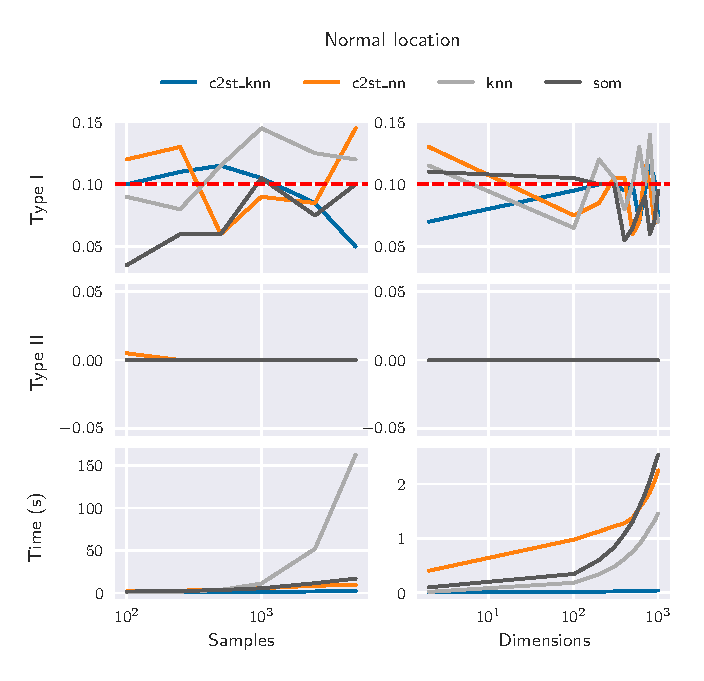
\includegraphics{images/6_som/normal_location}
    \caption{
    Location test for two multivariate Gaussian distributions with $D=1000$
    }
    \label{fig:normal_location}
\end{figure}

Figure~\ref{fig:normal_scale} shows the same variables for a scale test of two multivariate
Gaussian distributions with $D=1000$ and two random co-variances matrices samples from the
Wishart distribution~\cite{smith1972algorithm}. In this case, while the type I errors are
well bounded by the significance level, both algorithms based on neural networks
(C2ST-NN and \gls{SOM} ) require a higher number of samples to be able to reject $H_0$, with respect
to the other methods.

\begin{figure}[htbp]
    \centering
    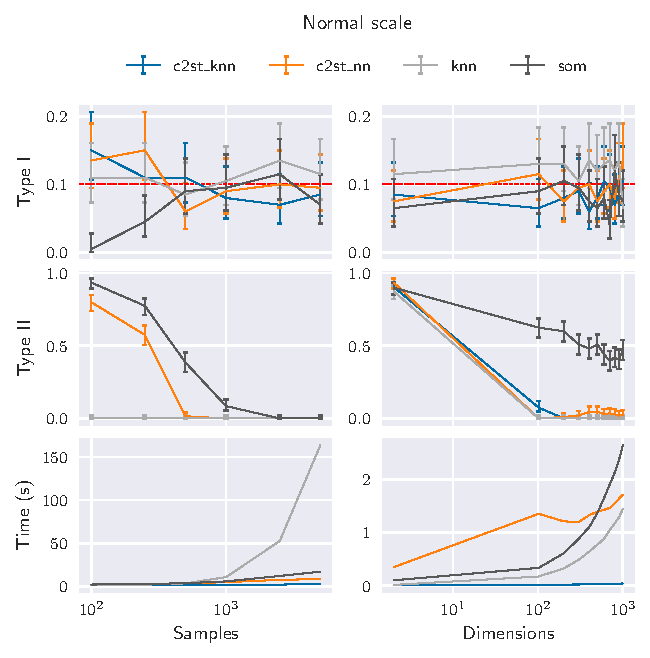
\includegraphics{images/6_som/normal_scale}
    \caption{Scale test for two multivariate Gaussian distributions with $D=1000$}
    \label{fig:normal_scale}
\end{figure}

Ramdas et al.~\cite{ramdas2015decreasing} have argued that a ``fair'' evaluation of the
power of multivariate non-parametric tests as the dimensionality increases is to keep the
amount of information fixed. i.e. the \gls{KLD} between both distributions
should remain constant.

For the location test, this can be achieved by two multivariate Gaussians that only differ
on the first dimension, i.e. $(1, 0, \ldots, 0)$ vs $(0, 0, \ldots, 0)$.

For completeness, figure~\ref{fig:normal_fair_location} shows the performance of the ML two-sample
tests being evaluated under this condition. We can see that, indeed, they all fail to improve
their type II error as the dimensionality increase.

\begin{figure}[htbp]
    \centering
    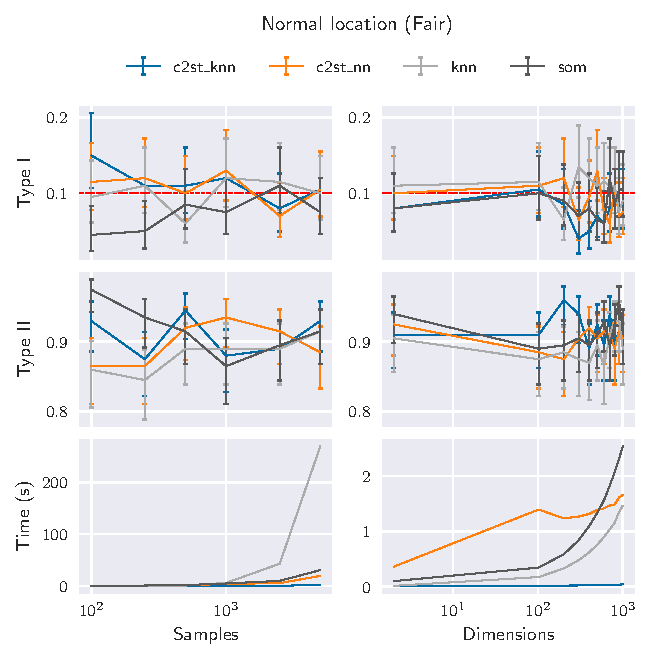
\includegraphics{images/6_som/normal_location_fair}
    \caption{Fair location test for two multivariate Gaussian distributions with $D=1000$}
    \label{fig:normal_fair_location}
\end{figure}

Finally, figure~\ref{fig:normal_fair_scale} shows the performance of the different
tests when only the scale of the first dimension differs, as Ramdas et al. propose
as a fair scale test. In this case it is more evident that the type II error of all
tests worsen as the number of the dimensions increase.

\begin{figure}[htbp]
    \centering
    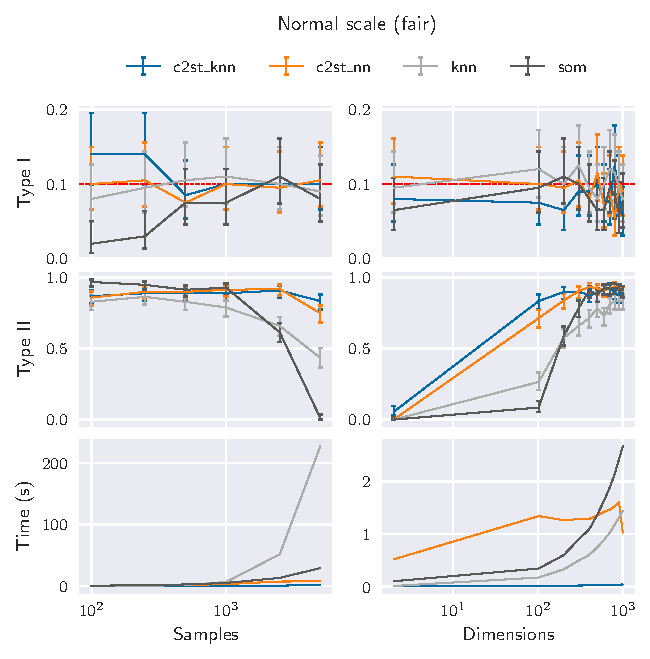
\includegraphics{images/6_som/normal_scale_fair}
    \caption{Fair scale test for two multivariate Gaussian distributions with $D=1000$}
    \label{fig:normal_fair_scale}
\end{figure}

We consider that Ramdas et al. raise a valid point: given the same amount of available
information, additional dimensions do not help. However, for our \PresQ use case this is an
unrealistic scenario: we are \emph{discovering} the matching dimensions, and each additional
feature will help in discriminating whether two samples follow the same distribution or not.

%%%%%%%
% DC2 %
%%%%%%%
\subsection{DC2}
The datasets from this challenge come from a single catalog of astronomical
objects, split based on the sky coordinates~\cite{EuclidDesprez2020}.

We generate three different samples:

\begin{enumerate}
    \item Samples from the full catalog
    \item Samples applying a magnitude cutout ($\text{MAG}_\text{VIS} < 22.)$
    \item Samples applying a signal-to-noise (SNR) cutout ($\text{VIS} / \text{VIS}_\text{Error} > 10.$)
\end{enumerate}

Following Ramdas et al. paper, in figure~\ref{fig:divergence_dc2} we report
the estimated \gls{KLD}~\cite{perez2008kullback} between the datasets for an
increasing number of dimensions. It can be seen that the amount of available information
rapidly increases for the magnitude cutout, but barely for the SNR one.

\begin{figure}[htbp]
    \begin{subfigure}[]{0.5\textwidth}
    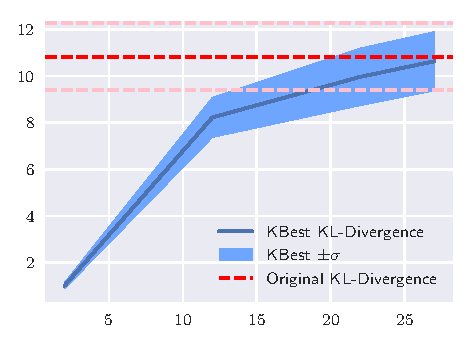
\includegraphics[width=\textwidth]{images/6_som/divergence/dc2_mag_divergence.eps}
    \caption{\gls{KLD} for the $\text{MAG}_\text{VIS}$ cutout}
    \end{subfigure}
    \hfill
    \begin{subfigure}[]{0.5\textwidth}
    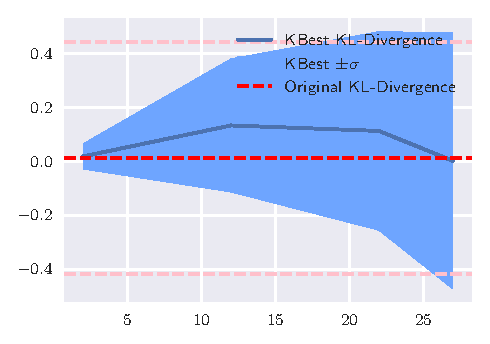
\includegraphics[width=\textwidth]{images/6_som/divergence/dc2_snr_divergence.eps}
    \caption{\gls{KLD} for the SNR cutout}
    \end{subfigure}
    \caption{\gls{KLD} for the DC2 samples}
    \label{fig:divergence_dc2}
\end{figure}

Figure~\ref{fig:dc2_mag} shows the measured performances for the DC2 with the magnitude
cutout. Even for a small sample size, the \gls{SOM}  test achieves very low type II errors, 
significantly better than the tests based on classifiers.
This may be due to the fact that the \gls{SOM} and kNN
tests can use the full sample while the classifiers must split the data into training and testing sets.


\begin{figure}[htpb]
    \centering
    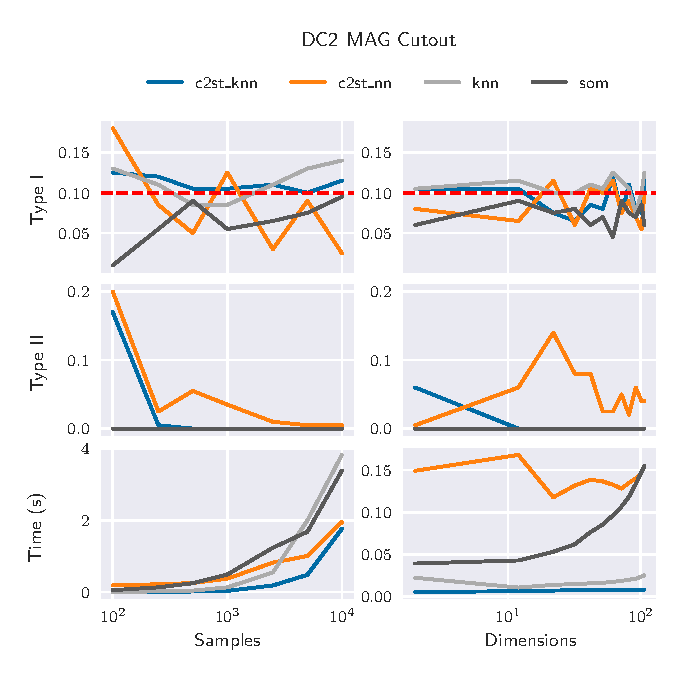
\includegraphics{images/6_som/dc2_mag}
    \caption{Statistical performance vs sample size (left) and dimensionality (right)}
    \label{fig:dc2_mag}
\end{figure}

Figure~\ref{fig:dc2_snr} shows the same performance metrics for the SNR cutout. In this case,
as suggested by the \gls{KLD}, adding dimensions does not help any of the tests.
However, as the sample size increases, both the \gls{kNN} and \gls{SOM}  tests achieve a good type II error rate,
while both classifiers remain with a high error rate.

\begin{figure}[htbp]
    \centering
    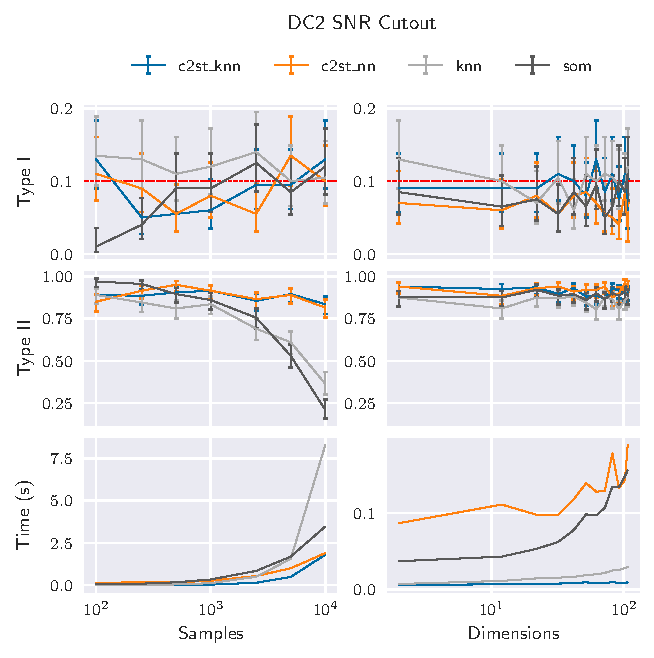
\includegraphics{images/6_som/dc2_snr}
    \caption{Statistical performance vs sample size (left) and dimensionality (right)}
    \label{fig:dc2_snr}
\end{figure}

\subsection{Open University Learning Analytics dataset}
\label{subsec:som_oulad}
The objective of this experiment is to prove that our proposed test can be successfully
used to test a hypothesis, providing an interpretable result, useful for further
investigating the data.

We base our test on the \emph{Open University Learning Analytics}
dataset, which contains anonymized data about student demographics~\cite{kuzilek_open_2017}.

Let us consider the case of a researcher with the hypothesis that gender, age, and
region of origin influence a student's economic situation, or perhaps they could
be trying to deanonymize the data.

From this dataset, we can use the \emph{Indices of Multiple Deprivations} (IMD) to measure poverty.
The null hypothesis $H_0$ would be that a sample from the overall population and a sample from
the poorest segment are indistinguishable, i.e., they come from the same distribution.

We take all students from the lower end of the poverty line and a sample of the same size
from the general population to test this hypothesis. We run the test using a \gls{SOM}  of size
$20\times20$. The null hypothesis is rejected with a p-value of $0$.

Unlike other statistical tests, in addition to the p-value, the researcher can use
the result of the \gls{SOM}  test to compare the projections of both samples.
Figure~\ref{fig:oulad_grid} shows the density of samples for each cell for the overall population
(left), the density of samples from the low-income students (center), and the relative difference
between both (right). The ``most different'' cells hint at how they are different.

\begin{figure}[t]
    \centering
    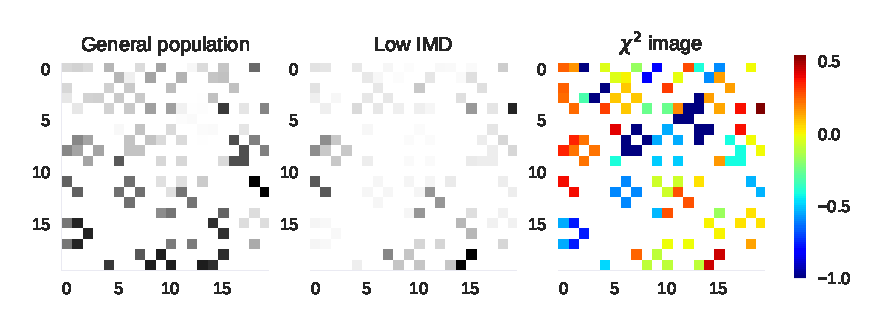
\includegraphics[width=\textwidth]{images/6_som/imd.eps}
    \caption[Comparing \gls{SOM} density variations]{Density of samples for the general population (left), poorest segment (center) and
    relative difference (right). Cells with a value of $-1$ do not have any low-income student,
    while those with a value of $0.5$ show an ``excess'' with respect to the general
    population.}
    \label{fig:oulad_grid}
\end{figure}

If we pick one of the cells with the most significant bias towards low-income students,
we can see it contains only young female students from the \emph{North Western Region}.
In figure \ref{fig:oulad_hist} we show the distribution of IMD for the overall population (left),
and for this subset (right). Indeed, the income distribution for this demographics is
heavily skewed towards the low end. We could obtain this hindsight without prior knowledge of which
attributes correlate with the difference, only with the ``hunch'' that
there is a relation. Thus, we prove that our proposed test can be useful for data exploration.

\begin{figure}[htbp]
    \centering
    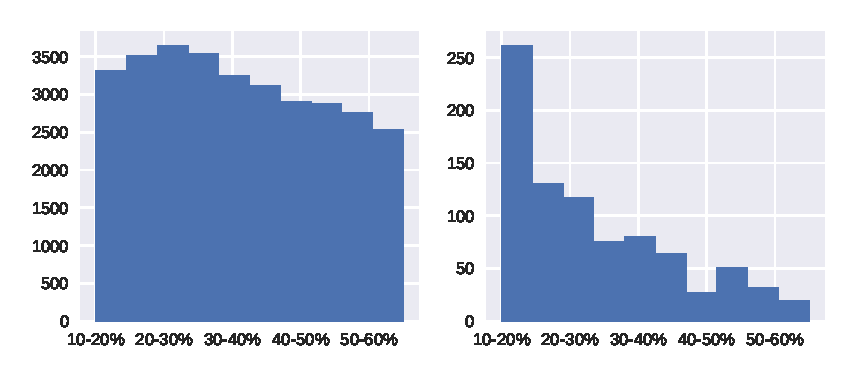
\includegraphics[width=\textwidth]{images/6_som/imd_histogram.eps}
    \caption[Histogram of the Indices of Multiple Deprivations for two populations]{
        \emph{Indices of Multiple Deprivations} for the general population (left) and for
        young female students from the \emph{North Western Region}.
    }
    \label{fig:oulad_hist}
\end{figure}

\subsection{Eye Movements}
\label{subsec:som_eye}
For generating this dataset, 11 subjects were shown a question and a list of ten 
associated sentences, of which one was the correct answer (C), four relevant (R), and five
irrelevant (I). Their eye movement was measured for each possible answer.
The overall measurements were summarized into 22 features, together with the
appropriate label for the sentence~\cite{salojarvi2005inferring}.

With this dataset, we aim to prove that our method can be competitive with other
start-of-the-art proposals, with the benefit of providing a trained model useful for
later purposes.

To evaluate the power of comparing different sets of measures, we replicate Song's
set up and run 2000 times\footnotemark the classifiers and \gls{SOM}  tests using a significance
level of $\alpha = 0.001$ for different sample sizes.
We report their statistical power on table \ref{tab:eye}. We have extracted the kernel-based
results from Song \etal paper~\cite{song2021fast}, including the second-best kernel
based method MMD-B~\cite{zaremba2013b}.

To evaluate the power of comparing different sets of measures, we replicate
Song's setup, and run 2000 times the classifiers and \gls{SOM}  tests
using a significance level of $\alpha = 0.001$ for different sample sizes.
We report their statistical power on table \ref{tab:eye}. The results from Song and
MMD-B are extracted from their paper~\cite{song2021fast}.

\footnotetext{Song uses 1000 repetitions.}

\begin{table}[htbp]
    \centering
    \begin{tabular}{c r r r r r r}
        \hline
        \multicolumn{7}{c}{\thead{I vs. C}} \\
        \hline
        \thead{m = n} & \thead{Song} & \thead{MMD-B} & \thead{KNN} & \thead{C2ST-KNN} & \thead{C2ST-NN} & \thead{SOM} \\
        \hline
        100 & 0.826 & 0.374 & \textbf{0.973} & 0.164 & 0.079 & 0.042 \\
        200 & 0.998 & 0.850 & \textbf{1.000} & 0.565 & 0.349 & 0.947 \\
        300 & \textbf{1.000} & 0.985 & \textbf{1.000} & 0.863 & 0.644 & \textbf{1.000} \\
        400 & \textbf{1.000} & \textbf{1.000} & \textbf{1.000} & 0.968 & 0.882 & \textbf{1.000} \\
        \\
        \hline
        \multicolumn{7}{c}{\thead{R vs. C}} \\
        \hline
        \thead{m = n} & \thead{Song} & \thead{MMD-B} & \thead{KNN} & \thead{C2ST-KNN} & \thead{C2ST-NN} & \thead{SOM} \\
        \hline
        100 & 0.670 & 0.236 & \textbf{0.845} & 0.062 & 0.023 & 0.007 \\
        200 & 0.969 & 0.685 & \textbf{0.996} & 0.298 & 0.139 & 0.672 \\
        300 & 0.999 & 0.941 & \textbf{1.000} & 0.558 & 0.314 & 0.987 \\
        400 & \textbf{1.000} & 0.988 & \textbf{1.000} & 0.811 & 0.560 & \textbf{1.000} \\
    \end{tabular}
    \caption{Empirical statistical power for the eye movement datasets}
    \label{tab:eye}
\end{table}

The results show that our test has low power for small samples, but it rapidly gains
terrain compared to the classifier-based methods, being competitive even with the
kernel-based techniques. The nearest-neighbors method is remarkably efficient in all cases.

To evaluate the usefulness of the trained model obtained as part of running the
statistical test, we use the trained \gls{SOM}  as a classifier by simply labeling
the input with a majority rule applied to each \gls{SOM}  cell. We performed a
50-fold cross-validation with a sample size of $n=m=409$, so each training set
is $n=m\approx 400$, corresponding
to the last entries in table \ref{tab:eye}.

The obtained mean accuracy where: C vs. I 68.42\%; C vs. R 67.84\%; I vs. R 53.90\%.
Even with relatively small sample sizes, our results are comparable with those
reported on the paper from which the dataset was obtained~\cite{salojarvi2005inferring}.

Finally, as an exercise on interpretability, figure~\ref{fig:eye_distinct_features}
shows the value of the two most distinct code-book dimensions. These attributes,
related to the regression (re-reading a word), show a sharp distinction that
matches the distribution of samples from the Correct and Incorrect samples quite
well.
Indeed, this matches the expectations from the original paper that the second-pass
measures indicate high-level cognitive processing and, therefore, correlate with
conscious efforts when choosing a correct answer.

\begin{figure}[htb]
    \centering
    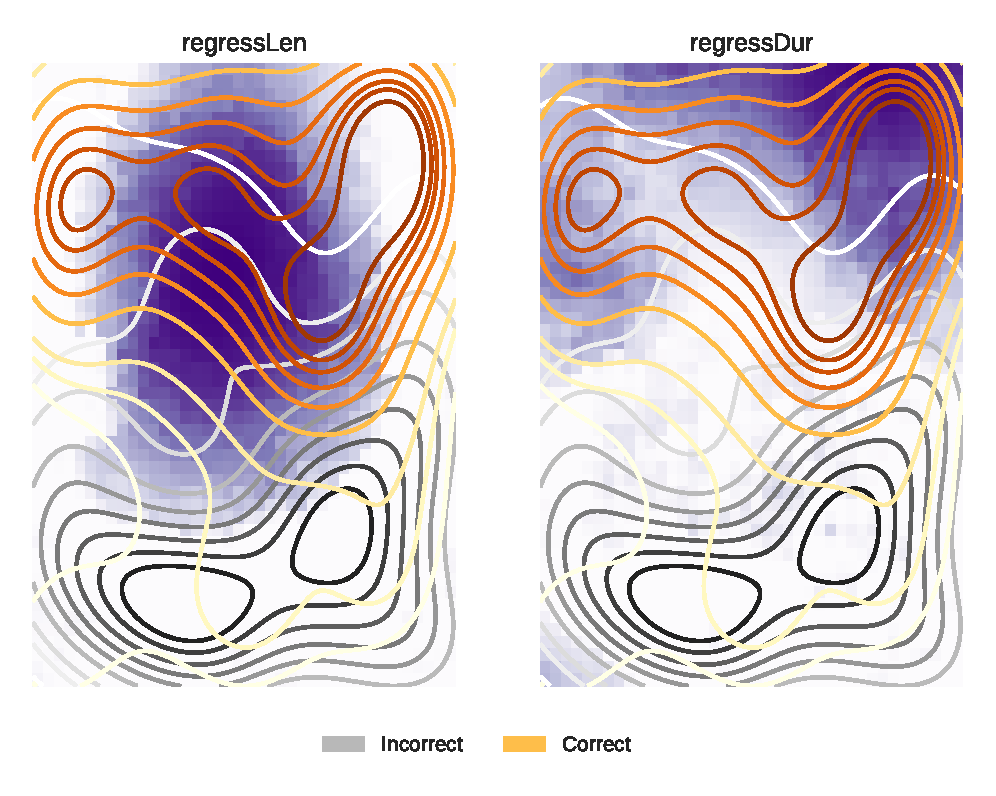
\includegraphics[width=\textwidth]{images/6_som/eye_regress.eps}
    \caption[Codebook values for the two most distinct features from the Eye dataset.]{
        Codebook values for the two most distinct features from the Eye dataset.
        Darker neurons are more sensitive to the given feature.
        The lines represent the density estimation for the Correct and \emph{Incorrect} samples over the \gls{SOM} .
        It is visible that the Incorrect category ``wraps'' around long regression distances, while the
        \emph{Correct} category correlates positively with the regression duration.
    }
    \label{fig:eye_distinct_features}
\end{figure}


\subsection{Age (IMDb Faces)}
The IMDb-WIKI dataset~\cite{rothe2018deep} contains 460,723 face images
extracted from IMDb. The authors additionally provide a neural network pre-trained
to predict the age of the face cutouts. Similarly to Song's experiments~\cite{song2021fast},
we have run the neural model over the IMDb faces, extracting the values from
the last hidden layer (4096 neurons) as the target multivariate distribution.

We then group the samples in age ranges, and verify our proposal comparing
500 samples from consecutive age groups, and repeat 500 times for each experiment. The
significance level is also set to $0.001$.

Table \ref{tab:age} shows the results for the \gls{SOM}  test, together
with the results reported by Song\etal for their kernel based method and for
MMD-B\cite{zaremba2013b}.

\begin{table}[htbp]
    \centering
    \begin{tabular}{lrrrr}
    \hline
    Age ranges & \thead{Song} & \thead{MMD-B} & \thead{KNN} & \thead{SOM} \\
    \hline
    15-20 vs. 20-25 & 1.000 & 1.000 & 1.000 & 1.000 \\
    20-25 vs. 25-30 & 1.000 & 0.800 & 0.984 & 0.990 \\
    25-30 vs. 30-35 & 0.990 & 0.790 & 0.876 & 0.726 \\
    30-35 vs. 35-40 & 1.000 & 0.830 & 0.866 & 0.812 \\
    35-40 vs. 40-45 & 0.950 & 0.250 & 0.784 & 0.564 \\
    40-45 vs. 45-50 & 0.930 & 0.400 & 0.812 & 0.606 \\
    \hline
    \end{tabular}
    \caption{Statistical performances for the Age dataset}
    \label{tab:age}
\end{table}

For this particular experiment Song's proposal outperforms both MMD-B and the \gls{SOM} 
test, although our method come second in statistical power.

%TODO: What about interpretability??

\subsection{\PresQ}
As we have mentioned in the introduction, the motivating example is the unsupervised
discovery of shared attributes between multiple datasets using \PresQ (chapter~\ref{chapter:presq}),
obtaining as a result the list of sets of attributes and a trained model that can be used to
cross-match the datasets.

We have run two examples from the \PresQ paper using the proposed \gls{SOM}  based test
instead of the \gls{kNN} statistical test. For each of the examples we measure:

\begin{description}
    \item[Ratio] of known shared attributes identified by \PresQ
    \item[Overhead] Number of tests per unique Equally-Distributed Dependency found
    \item[Time] that took \PresQ to finish, including the time taken for serializing the \gls{SOM}  models
\end{description}

Figure~\ref{fig:presq_som} reports the 95\% confidence interval ($\mu \pm 1.96 \sigma$)
for the \emph{relative differences} obtained when running with \gls{SOM}  vs
\gls{kNN}. Their distribution has been estimated using bootstrapping. The parametrization for
\PresQ was $\Lambda = 0.1$, $\gamma=0.95$, $\alpha=0.05$ and a sample size of 1000.

\begin{figure}[ht]
    \centering
    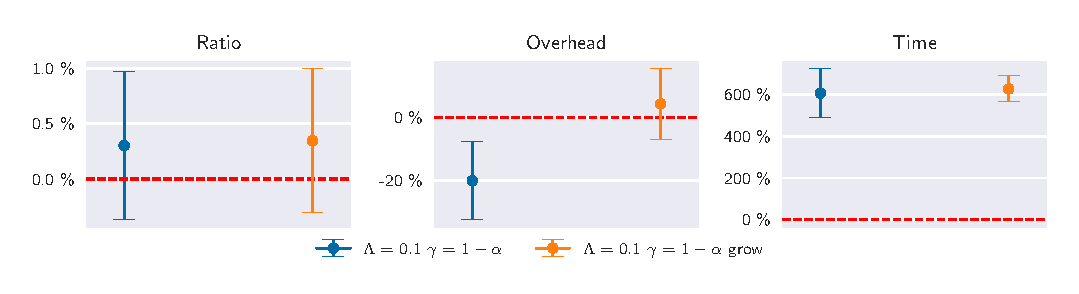
\includegraphics[width=\textwidth]{images/6_som/presq_som.eps}
    
    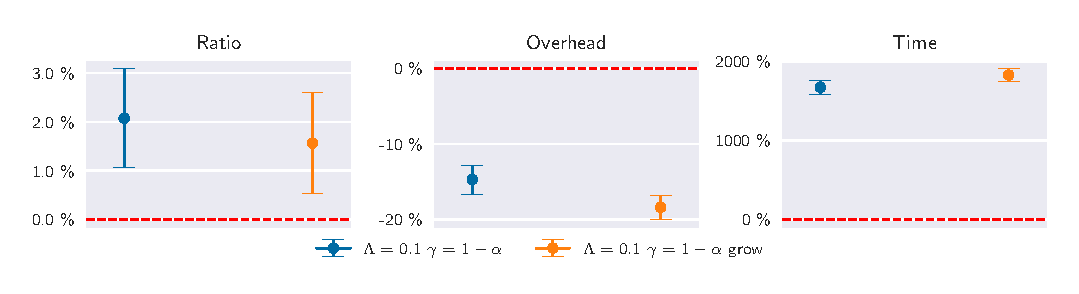
\includegraphics[width=\textwidth]{images/6_som/presq_som_aileron.eps}
    \caption[Relative difference between $\PresQ_{SOM}$ and $\PresQ_{kNN}$.]{
        Relative difference between $\PresQ_{SOM}$ and $\PresQ_{kNN}$.
        Top: DC2 dataset~\cite{EuclidDesprez2020}.
        Bottom: Ailerons / Elevators datasets~\cite{alcala2011keel}.
    }
    \label{fig:presq_som}
\end{figure}

The \gls{SOM}  test has a run-time penalty due to it being a more complex model to train.
However, for the same number of unique EDD found less tests are required. This is likely a consequence of
the $kNN$ test being slightly more prone to reject the equality of distribution than the \gls{SOM} 
test, as we can for instance see in figures \ref{fig:normal_location}, \ref{fig:normal_scale}.

\section{Conclusions}
\label{sec:som_conclusions}
As part of interactive data exploration, researchers may need to
compare multiple datasets.
These datasets can originate from multiple independent files or
generative models that need to be compared with reality. When these
datasets are of high dimensionality, especially if the exploration is
tentative, developing tailored statistical tests can become impractical.
In those cases, relying on heuristic approaches based on machine
learning techniques, as classifiers, to decide whether two samples are
distinguishable becomes a good
alternative~\cite{friedman2004multivariate,kim2021classification}.

However, some of these methods, like neural networks, are hard to interpret
when rejecting the null hypothesis $H_0: P = Q$. In other words, they
reject that both samples originate from the same underlying distribution,
but they do not assist the researcher any further.
Other models, such as random forests, are more  interpretable~\cite{friedman2004multivariate}.

In section~\ref{sec:som_chi2} we have proposed another machine learning
technique based on \glsfmtlongpl{SOM}~\cite{kohonen1982self} that is
understandable and capable of pointing the researcher to where the differences
in a multidimensional regime are. After all, \glspl{SOM} were initially
proposed as visualization aids. Nonetheless, they display interesting
emergent properties and can be used for clustering or classification as
well~\cite{ultsch2007emergence}.

In section~\ref{sec:som_results} we have proven that the power of this
technique is comparable to other machine learning techniques and even
superior for medium-size datasets.
We have also proven in the experiment~\ref{subsec:som_oulad} that the
output can guide researchers towards refining a hypothesis. Thus, our
test can be a valuable asset to the researcher's tool-set, and complementary
to more formal hypothesis testing whenever considered necessary~\cite{rosenblatt2021better}.

For future work, it would be interesting to explore the possibilities of
properties of emergent Self-Organizing Maps to assist the researcher
in examining the differences.
For instance, clustering could help identify whole regions that differ
rather than focusing on individual neurons.


\chapter{Discussion}
\label{chapter:discussion}

In section~\ref{sec:main_objective}, we defined that the main objective of this thesis
was \emph{to assist users during the exploration of unprocessed,
numerical, raw data distributed across multiple files}.
After a systematic literature mapping,
described in detail in chapter~\ref{chapter:literature_review}, in section~\ref{sec:objectives} we
narrowed the objectives to the \emph{multiple files with unknown, heterogeneous schemas, solely using the intrinsic data distribution}.

With this objective in mind, in chapter~\ref{chapter:diverse}
we proposed the concept of \gls{EDD},
proposed a novel algorithm, \PresQ, to mine these dependencies between multiple
datasets --- chapter~\ref{chapter:presq} ---, and a two-sample, machine-learning statistical
test that can visually assist users in examining how the two samples differ --- 
chapter~\ref{chapter:som}.

In section~\ref{sec:discuss_presq}, we discuss the behavior, performance, and results of
\PresQ, a tool for the discovery of multidimensional \glspl{EDD} via Quasi-Cliques
on Hypergraphs. In section~\ref{sec:discuss_som}, we argue how the
proposed solutions are relevant to the stated objectives. In
section~\ref{sec:threats}, we list the threats to the validity of this work and
what measures we have taken to minimize their impact.

\section{Discovery of Multidimensional Dependencies via Quasi-Cliques on Hypergraphs}
\label{sec:discuss_presq}

Identifying shared attributes between multiple numerical datasets is an interesting
problem. It combines the challenging nature of algorithms devised to find Inclusion Dependencies,
an NP-hard problem~\cite{kantola1992}, with the unavoidable uncertainty of statistical
methods.
This uncertainty reflects as falsely rejected \glspl{EDD} and falsely accepted \glspl{EDD}.

\Find is an algorithm that maps inclusion dependencies to hyper-cliques,
which generally performs  at least as well as the alternatives \cite{Dursch2019}.
It is loosely coupled with the discrete nature of the underlying data.
However, its ability --- and of most, if not all, of the existing algorithms --- to find
high arity \glspl{EDD} will be impaired by the number of false rejections,
which a lower rejection threshold could compensate for. Yet, this
solution increases the number of false detections, which is a known factor that 
significantly degrades its performance, similar to other hypergraph-based methods' \cite{koeller2006heuristic}.
We experimentally confirmed this problem in section \ref{sec:result_quasi_search}.

We propose a new algorithm based on quasi-cliques, where a candidate is accepted
even if some edges are missing. This algorithm has three parameters:

\begin{itemize}
    \item The ratio of missing edges ($\gamma$).
    \item The tolerance on the number of missing edges connecting a node from the quasi-clique ($\Lambda$).
    \item Whether to use the found quasi-clique as seeds.
\end{itemize}

We provide a generalization of this parameterization from regular 2-graphs
\cite{brunato2007effectively} to uniform $n$-graphs in equations~\ref{eq:edge_hyperclique}
and \ref{eq:deg_hyperclique}.

The results showed in the quasi-clique test set (section~\ref{sec:result_quasi_search})
demonstrate that the seed stage of \PresQ provides results close to the original
cliques on uniform $n$-hypergraphs. The growing stage
can recover them even for a high number of missing edges (up to $30\%$) at the expense of a higher run-time.
These results also prove that the degree threshold based on the hypergeometric distribution
offers comparable performance to a hand-picked ratio $\lambda$
while being more stable and predictable.

For real datasets, the ratio of missing edges can be intuitive to configure
(simply $\gamma = 1 - \alpha$, where $\alpha$ is the test significance level), 
but $\lambda$ can be harder to interpret. We propose instead an intuitive and statistically
interpretable method to dynamically adapt the threshold to the degree which is expected
to follow a hypergeometric distribution and can be adjusted based on the quasi-clique
itself, as shown in equation~\ref{eq:deg_hyperclique_hypergeom}.

While our tests on artificial hypergraphs seem to point to the redundancy of the parameter $\Lambda$,
the results shown in the real-world test set (section~\ref{sec:results_real}) prove that for real noisy graphs,
the combination of both performs consistently better than
either of them separately. The $\gamma$ parameter enables recovery from missing edges and,
simultaneously, $\Lambda$ avoids too many false positives due to 
spurious edges. Thanks to them, the efficacy can be kept even while maintaining or 
increasing the significance level of the tests. This reduces the risk of decreased
performance since the density of the graphs can be kept under control.

If a more exhaustive listing of maximal quasi-cliques is required, the initial set of
quasi-cliques can be used as \emph{seeds} to grow other quasi-cliques by adding suitable vertices.
The results shown in  section~\ref{sec:presq_experiments} demonstrate that this method is capable of
finding considerably more maximal quasi-cliques (not contained in any other found quasi-cliques)
at the expense of a higher run-time. This is due to the traversal of the search space and the
validation of the \glspl{EDD} represented by the quasi-cliques.

The loss of accuracy introduced by this growing stage is minor when starting at $n = 3$,
which means that the statistical test could not reject most candidates. However,
most candidates were rejected for an
initial $n = 2$. We consider this is mostly due
to the lack of power of the \gls{kNN} test for low dimensions, which introduces
many spurious edges.

The overall run-time of the \gls{EDD} finding algorithms is heavily influenced by the
chosen parameter values.
A strict parametrization will reject most seed candidates, and the quasi-clique search will fall
into exponential complexity. Conversely, a flexible one will be faster at finding
quasi-clique candidates. Yet, the statistical test will likely reject them, causing their decomposition
into an exponential number of newer, smaller candidates.
Generally, a balanced parametrization based on $\gamma$ and $\Lambda$ is more predictable.

As a final remark, the set of accepted \glspl{EDD} may contain several
false positives depending on the power of the multivariate statistical test.
A second, more detailed pass can refine this original set.
For instance, we can envision a ranking based on the previously discussed \emph{randomness}~\cite{Zhang2010}
to decide which set of \glspl{EDD} is more suitable for cross-matching the datasets.

In conclusion, \PresQ successfully identifies shared sets of attributes
between multiple data files containing raw, numerical data \emph{exclusively} based
on their distribution. This can guide users to cross-match datasets with unknown schemas,
but also to label attributes for which the metadata is lost as long as there is available
one dataset with properly labeled attributes.

Furthermore, \PresQ can also provide insights that drive serendipitous discoveries.
The \gls{AFDS} result shown in figure~\ref{fig:afds} is an example of such a case:
even with a set of files of unknown schema and unknown content, we could infer
a relation between samples confirmed by the paper that published the data.

\section{Two-sample test based on \glsfmtlong{SOM}}
\label{sec:discuss_som}
The results shown in section~\ref{sec:som_results} prove that the non-parametric,
two-sample \gls{SOM} test described in section~\ref{sec:som_chi2} generally outperforms,
in terms of power, other classifier-based two-sample tests, being in some cases
comparable to kernel-based methods. It has the added advantage of generating an
interpretable and usable model: for instance, the resulting \gls{SOM} could be used
as the basis for a \gls{SOM}-\gls{kNN} combined classification model~\cite{silva2011som}.

Like other machine-learning or kernel-based approaches, our method requires some
initial parameters, such as the \gls{SOM} size, to be set by the user. From our
tests, networks of size $O(100)$ neurons generally work well enough, but for more
precise control, the \gls{SOM} size can be set to the lengths of the two largest
principal components~\cite{KOHONEN201352}.

Rosenblatt \etal~\cite{rosenblatt2019better} argue that provable, \emph{proper} test statistics
should be, in general, preferred over heuristic alternatives. However, our
proposal is more oriented toward exploring abundant structured data. In this
case, developing a tailored statistic for all possible combinations is not viable,
and a pragmatic approach is more suitable~\cite{kim2021classification}.

Finally, if the null hypothesis --- that both samples come from the same underlying
distribution --- is rejected, the generated \gls{SOM}  model can be easily visualized
and examined in more detail.
In sections~\ref{subsec:som_oulad} and \ref{subsec:som_eye}, we demonstrated
that we can reject $H_0$ and obtain valuable information after exploring the learned model.
This exercise would not be possible with a black-box method such as
a neural network classifier~\cite{friedman2004multivariate}.

As a final note, \gls{SOM} maps can be generalizable to non-vectorial data
--- i.e., strings --- as long as more than one ordering relation is
defined~\cite{kohonen1982self, KOHONEN201352}.
Therefore, our proposed statistical test could also be used to verify whether
two sets of sequences --- i.e., proteins or DNA --- share their origin.
Unfortunately, since the \gls{SOM} implementation on which we based our implementation
only works with real-valued dimensions~\cite{wittek_somoclu_2017}, we were not
able to test this scenario.

\section{Threats to validity}
\label{sec:threats}

We now identify the internal and external
threats to the validity of our research, and the measures we took to
counteract their effect.

\subsection{Internal validity}

The \PresQ results shown in the experiments described in section~\ref{sec:presq_experiments}
could risk being just a fluctuation,
not due to an underlying algorithmic improvement. However,
the experimental design described in section~\ref{sec:experiment_design} significantly reduces
this possibility, thanks to the randomization of the initial conditions
and the number of measurements. In any event, we made explicit the uncertainties
of our results --- using 95\% confidence intervals or reporting distribution quartiles.

The results summarized in table~\ref{tab:ind2_summary} show that, on average, the
quasi-clique-based searching algorithm consistently performs
better both in terms of run-time and ability to find the maximal \gls{EDD}.
It has enough runs to make the difference significant.
It is worth mentioning that there are proposed heuristics~\cite{koeller2003discovery} to find higher
arity \glspl{EDD}, even when edges are missing, by merging found lower-arity
\glspl{EDD} and testing the resulting \gls{EDD} candidate.
Nonetheless, we consider that the run-time differences are significant enough to make
the quasi-clique-based search a better approach in those cases.
Even so, that heuristic can also be applied to the output of our proposed algorithm.

We implemented \Find and \PresQ from scratch, sharing 
many parts of the code --- i.e., data structures, statistical tests, etc.
While there is room for optimizations, both would benefit.
Since the relative differences would remain similar, we are confident that the gains come from the 
algorithm rather than its implementation.

\medskip

For the proposed two-sample statistical test, the results shown in
section~\ref{sec:som_results} originate from running the tests between 200 and 2000
times, with independent randomized samples.
Again, the comparisons took into account the error in our measurements,
making it easier to assess their significance.

\subsection{External validity}
The \PresQ experiments were run over four different datasets of
diverse nature and from three separate sources. The chosen statistical tests for
uni- and multi-dimensional distributions were not customized to any of them.
However, a better statistical test can be used if the underlying data distribution is more or
less known (or suspected), which may reduce, or even remove, the advantage of the
quasi-clique approach. Although it is also unlikely that the performance would be any worse:
since an entire clique is still a quasi-clique, our algorithm can identify all of them,
similar to the original \Find algorithm.

One significant caveat of our approach is that it may not find
any dependencies if prior filtering has been applied to only one of the two relations
(i.e., signal-to-noise filtering). This is a limitation of the validation
step. This issue was also recognized on the original \Find proposal \cite{koeller2003discovery}.

\medskip

Similarly, the experiments for the two-sample statistical test based on \gls{SOM}
were run over five different datasets and compared with kernel-based and machine-learning-based
alternatives. Given the performance shown by this test, we are confident in
its capabilities.


\chapter{Conclusions and Future Work}
\label{chapter:conclusions}
\glsresetall

\section{Summary}

\emph{In situ} Data Exploration is an active research area that requires
a multidisciplinary approach: algorithms, data structures, machine learning,
statistics,  data visualization, information sciences, and, unavoidably,
the domain knowledge --- or business understanding ---  provided by an expert.

Going back to the \gls{CRISPDM} model described in  chapter~\ref{chapter:introduction}
and shown in figure~\ref{fig:crispdm}, our initial objective was to identify
gaps in the tooling available for experts to understand data coming as a set of
unprocessed and perhaps inconsistent set of files. These files are not optimized
for access, and any early decision on how to ingest them into a database may be
counterproductive until the dataset is better understood.

The literature survey from chapter~\ref{chapter:literature_review} showed that
solutions for visualization, optimizations, indexing, storage,\ldots abound.
Still, there is little to no mention of assisting users on \emph{understanding}
data schema, especially when it comes to multiple files from diverse origins or
when meta-data is incomplete or inconsistent.
In chapter~\ref{chapter:diverse}, we have seen that users spend a non-negligible
amount of resources just examining the data structure and layout.

The question that followed was: can we leverage the data \emph{distribution} to
assist users in understanding the schema, on seeing how different datasets may come together?
This is particularly important when the data is numerical and uncertain since
one can not just compare tuples individually but needs to inspect distributions.

In the relational world, the \gls{IND} concept comes close to the objective:
parts of a relation contained (included) within another. However, this modeling
relies on the attributes' discrete nature, such as name, date of birth, etc.

In chapter~\ref{chapter:presq} we propose a generalization, the \gls{EDD}, that
relaxes the strict containment relation required by \glspl{IND}.
We then introduce \PresQ, a novel algorithm for \gls{EDD} finding that incorporates
uncertainty into its world modeling, proving that relying on data distribution alone is feasible.
Therefore, \PresQ is applicable in situations where most existing \gls{IND} solutions
are not: when the data is intrinsically uncertain --- measures of physical properties ---,
or when the validation strategy for the inclusion is an approximate heuristic.
The only requirement is that the expectation of false negatives --- i.e., significance
level for statistical tests --- can be estimated.

For the experiments used to evaluate \PresQ, described in ~\ref{sec:presq_experiments},
the statistical test of choice was based on the $k$-nearest neighbors. While this test
performs well for a wide range of datasets, the resulting trained \emph{model} is not
very useful.
Chapter~\ref{chapter:som} introduces a statistical test based on \gls{SOM}, which provides,
in addition to a $p$ value, a trained projection that we can later use for binning and
cross-matching both datasets using the matching set of features. The resulting \gls{SOM}
is also interpretable in case of rejection, which is also helpful in tentative data exploration.

\section{Contributions}

\subsection{Publications}
\begin{refsection}
\nocite{Alvarez2019,Alvarez2021inference,AlvarezAyllonPresQ2022}

\printbibliography[heading=none]
\end{refsection}

\subsection{Software}
\todo{Software (PresQ)}

\section{Future work}
\todo{Is it worth to mention dead-ends? i.e., structure on Probabilistic Graphical Networks}

\begin{itemize}
    \item In chapter~\ref{chapter:presq}, we prove that finding quasi-cliques in hypergraphs
    is a successful technique to find \gls{EDD}, or \gls{IND} based on approximate heuristics
    between relations. Therefore, a place for further research is to
    \textbf{improve the quasi-clique finding} algorithm, either via novel algorithms or by
    generalizing some of the many existing techniques~\cite{WU2015693}.
            
    \item On the other hand, the existing algorithms based on quasi-clique search forget
    about certain aspects of the datasets. For instance, the correlation matrix on both
    sides of the \gls{EDD} is likely to be similar, and it may be possible to leverage
    \textbf{data-aware} algorithms to augment the quasi-clique finding.
    
    \item Sometimes, the algorithms should not assume equality-of-distribution. For instance, one of the
    datasets may have been filtered beforehand --- i.e., signal-to-noise, value clipping, etc. This issue affects
    both \gls{EDD} and \gls{IND} algorithms~\cite{koeller2003discovery}. \textbf{Partial inclusion/equality-of-distribution}
    remains an open problem.
            
    \item \PresQ is based on frequentist probability, which does not allow incorporating \textbf{prior beliefs}
    into the algorithm. i.e., a \textbf{domain-expert} has no way of influencing the result based
    on her knowledge of the area.
    A Bayesian framework could prove helpful in this respect. Furthermore, in relation with the previous point,
    it can also be used to perform local null hypothesis testing~\cite{soriano2015bayesian}, which could help
    identify partial \glspl{EDD} --- as when a filter has been applied to one of the datasets.
    
    \item Searching for quasi-cliques involves exponential time complexity on the number of nodes.
    Thus, beforehand, applying a \textbf{dimensionality reduction} would reduce the total
    run-time and decrease the noise. Nonetheless, a complication arises from the premise that
    we do not know which attributes are shared.
        
    \item Finally, \textbf{finding other types of numerical dependencies} can be of interest.
    For instance, a single dataset may be split between multiple files based on the values
    from a given set of attributes, which may or may not overlap.
    As an example, figure~\ref{subfig:tu_multifile} shows an example where a single dataset is
    cleanly cut using two spatial dimensions, which can be easily \emph{learned} by a decision tree.
    Figure~\ref{subfig:mer_multifile} shows another dataset also cut using the same two
    coordinates, but where there exists an overlap between some of the files.
\end{itemize}

\begin{figure}[htbp]
    \begin{subfigure}[]{0.5\textwidth}
    \includegraphics[width=\textwidth]{images/8_conclusions/tu_multifile_tree.png}
    \caption{Without overlap}\label{subfig:tu_multifile}
    \end{subfigure}
    \hfill
    \begin{subfigure}[]{0.5\textwidth}
    \includegraphics[width=\textwidth]{images/8_conclusions/mer_multifile_tree.png}
    \caption{With overlap}\label{subfig:mer_multifile}
    \end{subfigure}
    \caption{
        Data-sets distributed multiple files based on two spatial coordinates.
        Each color corresponds to a single file.
    }
    \label{fig:tree_cat_cut}
\end{figure}


% Bibliography
\printbibliography[heading=bibintoc,segment=0]

% Appendices
\appendix
\newrefsegment

\chapter{\PresQ Benchmarking Tools}
\label{appendix:presq_benchmarks}
The repository \texttt{MatchBox}\footnote{\url{https://github.com/ayllon/MatchBox/}}
contains the Python implementation of \PresQ and \Find used as a reference for the
performance comparison shown in chapter~\ref{chapter:presq}, together with instructions
to reproduce the results.

For facilitating the replicability of the results, the repository contains an \linebreak
\texttt{environment.yml} file that allows re-creating a working Python environment
with all the requirements installed using \href{https://docs.conda.io/en/latest/}{\texttt{Conda}}:

\begin{minted}{bash}
conda env create
conda activate matchbox
\end{minted}

\section{Benchmarking quasi-clique finding}

\texttt{benchmark-quasiclique.py} compares the performances of \Find (baseline) and \PresQ
when searching for a known quasi-clique generated randomly based on an initial parameterization:
rank, cardinality, the ratio of missing edges, the number of nodes not belonging to the
quasi-clique, and the ratio of spurious edges. The results are written to a \gls{CSV} file.

The script snippet~\ref{script:quasi_missing} shows the relevant extract used to evaluate
the capacity of \PresQ to recover from missing edges, as reported in figure~\ref{fig:3hyper_alpha}.

\begin{code}
\caption[Benchmark quasi-clique search with a set of missing ratios.]{
Benchmark quasi-clique search with a set of missing ratios. The comments need to be removed.}\label{script:quasi_missing}
\begin{minted}{bash}
for alpha in 0.05 0.10 0.15 0.20 0.25 0.30; do
  ./bin/benchmark-quasiclique.py \
    --out "results/quasi3.csv" \ # Output CSV
    --rank 3 \                   # 3-hypergraph
    --cardinality 10 20 30 \     # Number of nodes on the quasi-clique
    --additional 0.5 \           # |V| * 0.5 additional nodes
    --repeat 15 \                # Generate 15 different hypergraphs
    --missing-edges ${alpha} \   # Remove $alpha edges from the quasi-clique
    --extra-edges 0 \            # Do not add any spurious edge
    --timeout 300                # Limit execution to 5 minutes
done
\end{minted}
\end{code}

On the other hand, snippet~\ref{script:quasi_spurious} shows the call used to evaluate
the capacity of \PresQ to recover from both missing and spurious edges, as reported in
figure~\ref{fig:hyper_ab_corr}. The set of spurious edges $S$ contains \emph{all} possible edges
on the hypergraph \emph{not} belonging to the quasi-clique.

\begin{code}
\caption[{Benchmark quasi-clique search with a set of additional edges.]{Benchmark quasi-clique search with a set of additional edges. The comments need to be removed.}\label{script:quasi_spurious}
\begin{minted}{bash}
for beta in 0.2 0.4 0.6 0.8; do
  ./bin/benchmark-quasiclique.py \
    --out "results/quasi3.csv" \ # Output CSV
    --rank 3 \                   # 3-hypergraph
    --cardinality 10 20 30 \     # Number of nodes on the quasi-clique
    --additional 0.5 \           # |V| * 0.5 additional nodes
    --repeat 15 \                # Generate 15 different hypergraphs
    --missing-edges 0.1 \        # Remove 10% of edges from the quasi-clique
    --extra-edges ${beta} \      # Add $beta * |S| spurious edges
    --timeout 1200               # Limit execution to 20 minutes
done
\end{minted}
\end{code}

\section{Benchmarking \glsfmtlong{EDD} finding}

\texttt{benchmark.py} is a script that can be used to measure the performance of
\PresQ and the custom implementation of \Find over datasets available in any of
the supported formats: \gls{FITS}, \textsc{KEEL} \texttt{.dat} files, \gls{CSV},
and \textsc{SQLite}.
The script needs a minimum of two relations and supports running multiple
parameterizations of \PresQ with a single invocation.

The measurements are written to a set of \gls{CSV} files:

\begin{center}
\resizebox{\textwidth}{!}{%
    \begin{tabular}{r|l}
    \thead{Name} & \thead{Description} \\ \hline
    \texttt{sampling.csv}  & Sampling time \\
    \texttt{uind.csv}      & Statistics about unary EDD \\
    \texttt{bootstrap.csv} & Statistics about initial edges tested and accepted \\
    \texttt{find2.csv}     & \Find runs \\
    \texttt{findg\_\{$\Lambda$\}\_\{$\theta$\}\_\{grow\}.csv} & \PresQ runs with different parameterizations \vspace{1em} \\
    \texttt{\{uuid[0:2]\}/\{uuid\}/histogram.txt} & Histogram of the EDD arity found for run \texttt{uuid} \\
    \texttt{\{uuid[0:2]\}/\{uuid\}/nind.txt} & List of EDD found for run \texttt{uuid}
\end{tabular}}
\end{center}

Note that the effective value of $\gamma = 1 -\alpha \times \theta$. i.e, \texttt{findg\_0.05\_1.00\_1.csv} contains
the results for a run of \PresQ with $\Lambda = 0.05$, $\gamma = 1 - 0.1 \times 1 = 0.9$ (for $\alpha = 0.1$),
and the growing stage enabled.

\subsection{\Find vs. \PresQ}

The snippet~\ref{script:edd_finding} shows, as an illustration, how the comparison for the
datasets \texttt{Ailerons vs Elevators} was executed for table~\ref{tab:ind2_summary}.
For completeness, it also shows the parameters that kept their default values.

\begin{code}
\caption[Benchmark \Find vs. \PresQ over the \texttt{Ailerons vs Elevators} datasets.]{
Benchmark \Find vs. \PresQ over the \texttt{Ailerons vs. Elevators} datasets. The comments need to be removed.}\label{script:edd_finding}
\begin{minted}{bash}
ID="ailerons_$(date +%Y%m%d)"

./bin/benchmark.py \
    --output-dir "./results/" \ # Write the results to this directory
    --id "${ID}"              \ # Under the given folder name
    --repeat 1000             \ # 1000 randomized runs
    --timeout 3000            \ # With a timeout of 50 minutes for one run
    --sample-size 200         \ # Sample size (DEFAULT)
    -k 3                      \ # Neighbors for the kNN test (DEFAULT)
    --permutations 500        \ # Permutations for the kNN test (DEFAULT)
    --nind-alpha 0.05         \ # Significance level for EDDs (DEFAULT)
    --bootstrap-arity 2       \ # Rank for the initial hypergraph (DEFAULT)
    --lambdas 0.05 0.1        \ # PresQ parameter Lambda (DEFAULT)
    --gammas 1.               \ # gamma = 1 - alpha * 1 (DEFAULT)
     # Significance levels for initial edges/2-EDD (DEFAULT)
    --bootstrap-alpha 0.05 0.1 0.15 \
    "./data/keel/ailerons/ailerons.dat" \
    "./data/keel/elevators/elevators.dat"
\end{minted}
\end{code}

\subsection{Scalability}

The snippet~\ref{script:perf_columns} corresponds to the performance evaluation shown
in figure~\ref{fig:scalability}, where new relations are incrementally added to measure
the scalability of \PresQ with respect to the number of attributes.
One instance of \textsc{ChemBL} contains 80 relations. Note that the script
originally expected one file per relation; thus, the \texttt{SQLite} back-ends abuses
nomenclature for the parameter \texttt{--files}.

\begin{code}
\caption[Benchmark performance with respect to the number of columns.]{
Benchmark performance with respect to the number of columns. The comments need to be removed.}\label{script:perf_columns}
\begin{minted}{bash}
ID="chembl_$(date +%Y%m%d)"

for i in {82..160..6}; do       # From 82 to 160 relations
  ./bin/benchmark.py \
    --output-dir "./results/" \ # Write the results to this directory
     --id "${ID}"             \ # Under the given folder name
    --repeat 10               \ # 10 randomized runs
    --timeout 3000            \ # With a timeout of 50 minutes for one run
    --lambdas 0.1             \ # PresQ parameter Lambda
    --bootstrap-alpha 0.05    \ # Significance levels for initial edges/2-EDD
    --no-find2                \ # Do not run Find2 in this case
    --files $i                \ # Number of relations
    --sample-size 200         \ # Sample size (DEFAULT)
    -k 3                      \ # Neighbors for the kNN test (DEFAULT)
    --permutations 500        \ # Permutations for the kNN test (DEFAULT)
    --nind-alpha 0.05         \ # Significance level for EDDs (DEFAULT)
    --bootstrap-arity 2       \ # Rank for the initial hypergraph (DEFAULT)
    --gammas 1.               \ # gamma = 1 - alpha * 1 (DEFAULT)
    ./data/chembl/chembl_??.db
done
\end{minted}
\end{code}


\chapter{Prototypes Overview}
\label{appendix:prototypes}
Iterating over a set of ideas is an intrinsic part of both the
\emph{Engineering Design Process} and research, and some end being discarded.
Nevertheless, knowing about the discarded paths can be helpful~\cite{conroy_three_2020}
since they can point to either future lines of work or dead-ends not worth pursuing.

In this appendix, we briefly describe one insight and two prototypes generated during
the development of this thesis that did not prove successful.

\section{Types of Data Correlation}

In 2017, \cite{Kraska2017} proposed a novel idea: an index over a dataset
is just a model. This model takes as input a value, or a range of values,
and ``predicts'' the physical location of the corresponding tuples.
In this work, Kraska \etal propose \emph{learned} alternatives to well-known data
structures often used on databases for different access patterns:
value range (typically modeled with B-trees), unique values (hash tables),
and existence queries (Bloom filters).
However, Kraska \etal trained models over a single attribute.
Extending these types of models might also be possible when multiple files exist.

Thus, based only on the data, we can learn models to predict the value of
other attributes --- i.e., what we normally understand by machine learning ---,
the file where it is stored, and its offset.
This is possible under the assumption that there are three types of \emph{correlations}
or \emph{dependencies}:

\begin{itemize}
    \item \textbf{File Correlation} Dependence between values and containing file.
    \item \textbf{Offset Correlation} Dependence between values and offset within the
        file~\cite{Kraska2017}.
    \item \textbf{Tuple Correlation} Dependence between the attribute values of a tuple.
\end{itemize}

Note that the first two correlations depend on the acquisition method, and the third
on the measured properties.

\PresQ builds on the third assumption in order to find \glspl{EDD}: same set of attributes
from the same population follow the same distribution.

We now describe an attempt to leverage the first type of correlation in
section~\ref{sec:file_correlation}, a naive indexing approach on section~\ref{sec:offset_correlation},
and an early prototype for schema matching in section~\ref{sec:attribute_correlation}.

% See informe 2020 for details
\section{File Correlation}
\label{sec:file_correlation}

Large datasets may be partitioned into multiple files to facilitate their use.
This partitioning can be done as a function of some data features: spatial coordinates,
alphanumerical order, temporal order, etc. Therefore, machine learning techniques
should be able to model (index) this partitioning without user intervention.

As a proof-of-concept, we took two astronomical catalogs partitioned into multiple
files generated by two different processes: simulation and measurement.

We can see the indexing as a ``classification'' task: we want to model the file (label)
corresponding to a given data set. For the feature selection, we use Random Forest
with 100 trees. Features with higher weight are those used to partition the data.
Code~\ref{code:sel_attr_multifile} shows an snippet of the feature selection.
We executed it over a random sample of 5000 tuples per file.
We obtained that the sky coordinates --- right ascension and declination --- were
the best features for both the simulation and the measurement catalogs.

\begin{listing}[H]
\begin{minted}[linenos]{python}
# feat_cols contains all features except the file index
classifier = RandomForestClassifier(n_estimators = 100)
classifier.fit(train[feat_cols], train['FILE'])
# Contains the weight for each feature
classifier.feature_importances_
\end{minted}
\caption{Feature selection for file correlation}
\label{code:sel_attr_multifile}
\end{listing}

Since trees are a data structure commonly used for spatial partitioning
--- KD-Tree, Binary Partition Tree, R-Tree --- we trained two decision trees over
both catalogs using the sky coordinates as features.
We display the resulting ``learned'' partitioning over the actual data distribution
in figure~\ref{fig:tree_cat_cut}.
We can see that in the simulated catalog, the prediction is very accurate.
However, the results are suboptimal over the real-world catalog due to overlapping catalogs.
This issue could be fixed by training a binary classifier by file.

\begin{figure}[htbp]
    \begin{subfigure}[]{0.5\textwidth}
    \includegraphics[width=\textwidth]{images/A2_prototypes/tu_multifile_tree.png}
    \caption{Without overlap}\label{subfig:tu_multifile}
    \end{subfigure}
    \hfill
    \begin{subfigure}[]{0.5\textwidth}
    \includegraphics[width=\textwidth]{images/A2_prototypes/mer_multifile_tree.png}
    \caption{With overlap}\label{subfig:mer_multifile}
    \end{subfigure}
    \caption{
        Data-sets distributed multiple files based on two spatial coordinates.
        Each color corresponds to a single file.
    }
    \label{fig:tree_cat_cut}
\end{figure}


\section{Offset Correlation}
\label{sec:offset_correlation}

We work with the assumption that the data acquisition method influences
the data distribution within a file. Although this correlation is not always
true, we expect it to be for raw data.

To validate the idea, we obtain random samples from three astronomical catalogs
(\gls{Cosmos}\cite{laigle2016cosmos2015}, \gls{SDSS}\cite{SDSS14}, and \gls{KiDS}\cite{de2013kilo}),
all extracted from the same sky region.

As for the file correlation case, the best features are sky coordinates.
The target variable is the page offset within the file, which we obtained via code~\ref{code:page}.
Rather than training a simple regression model and predicting the exact page, we trained models
capable of predicting a page range: \textit{Quantile Regression Forests}~\cite{meinshausen2006}
and \textit{Gradient Boosting}~\cite{mason2000}.
The training set comprises 10\% of the tuples (1\% for Cosmos given its size), and the test
set 20\% of the remaining tuples.

The same test were run over a non astronomical data-set\footnote{\url{https://www.kaggle.com/sobhanmoosavi/us-accidents}}, for which
the best features are \texttt{Start\_Time}, \texttt{End\_time} and
\texttt{Weather\_Timestamp}\footnote{\texttt{ID} is a better feature, but arguably not very interesting.}.

\begin{listing}[htpb]
\begin{minted}[linenos]{python}
block_size = os.statvfs("/path/to/files").f_bsize
row_size = np.array(table[0:1]).nbytes
page = (np.arange(len(table)) * row_size) // block_size
\end{minted}
\caption{Computation of the page offset}
\label{code:page}
\end{listing}

Table~\ref{tab:offset_prediction} summarizes the results of both models
for the four datasets. \textit{Quantile Regression Forests} can be accurate --- it predicts
the correct range --- but the overhead is not negligible --- it needs to read
a considerable portion of the file per prediction.

\begin{table}[htpb]
    \begin{tabularx}{\linewidth}{X l c r r r}
    \thead{Catalog} & \thead{N.Pages} & \thead{Method} &
    \thead{Time (s)} & \thead{Accuracy} & \thead{Precision}\\
    \hline

    \multirow{2}{*}{Cosmos} & \multirow{2}{*}{78 499} &
        QRF &  16.69 & 94.30\% & 0.39\% (306) \\
    & & GB  & 128.07 & 63.30\% & 1.57\% (1236)  \\

    \hline

    \multirow{2}{*}{SDSS} & \multirow{2}{*}{1 825} &
        QRF &  6.86 & 95.74\% & 6.53\% (119) \\
    & & GB  & 21.28 & 60.73\% & 3.15\% (57) \\

    \hline

    \multirow{2}{*}{KiDS} & \multirow{2}{*}{7 773} &
        QRF &  8.62 & 97.37\% & 0.36\% (28) \\
    & & GB  & 41.22 & 62.33\% & 1.63\% (127) \\
    
    \hline
    
    \multirow{2}{*}{Accidents} & \multirow{2}{*}{261 193} &
        QRF &127.56 & 84.86\% & 19.11\% (49926) \\
    & & GB  &  9.13 & 61.00\% & 14.10\% (36820) \\
    
    \end{tabularx}
    \caption{QR vs GBR over different datasets.
    \emph{Time}: Training time
    \emph{Accuracy}: Ratio of predicted ranges that contain the queried tuple.
    \emph{Precision}: Average range size with respect the total file size.}
    \label{tab:offset_prediction}
\end{table}


\section{Attribute Correlation}
\label{sec:attribute_correlation}

Within a relation, we expect some attributes to be closely correlated.
This correlation is inherent to the attributes and the sampled population.
Thus, two files containing samples for the same attributes from the same
underlying population should display a similar.

This correlation is intrinsic to the data and independent of the physical
schema of the data --- i.e., file layout or attribute names. Alternatively,
two datasets with different schemas but containing a similar subset of
measures should show the same dependencies between attributes. We can
expect to use these dependencies to match schemas\footnotemark.

\footnotetext{This insight directed the research toward the Equally-Distributed-Dependencies.}

Since Bayesian networks~\cite{pearl1988}  model the data dependencies
as a directed acyclic graph, we can expect that graphs trained over different
datasets containing the same information should be similar.

For validating the idea, we have trained three Bayesian networks using
\textsc{Pomegranate}~\cite{schreiber2018pomegranate} over the catalogs
\gls{SDSS}, \gls{KiDS} and \gls{Cosmos}. Figure~\ref{fig:bayes1} shows the
resulting graphs for the first two, and figure~\ref{fig:bayes2} for the last.

Indeed, these graphs are significantly similar for \gls{SDSS} and \gls{KiDS},
even on the order of the bands. This match is less evident for \gls{Cosmos},
given the different bands in the catalog. However, the correspondence is
remarkable if we consider the physical order of the bands --- shown in table~\ref{tab:bandas}.

However, there remain two problems:

Most existing algorithms do not support learning Bayesian networks over continuous features,
and it is necessary to discretize them first. If this approach is not enough, there are some
proposals to train Bayesian networks using a combination of continuous and discrete
variables~\cite{Lucas2015,chen2017}.

There needs to be more than the correspondence between nodes in the graphs to compute
the correspondence between attributes. The Bayesian networks may not be stable, with
attributes changing relative positions or relations being missed.

\begin{figure}[htpb]
    \centering
    \begin{subfigure}[]{\textwidth}
    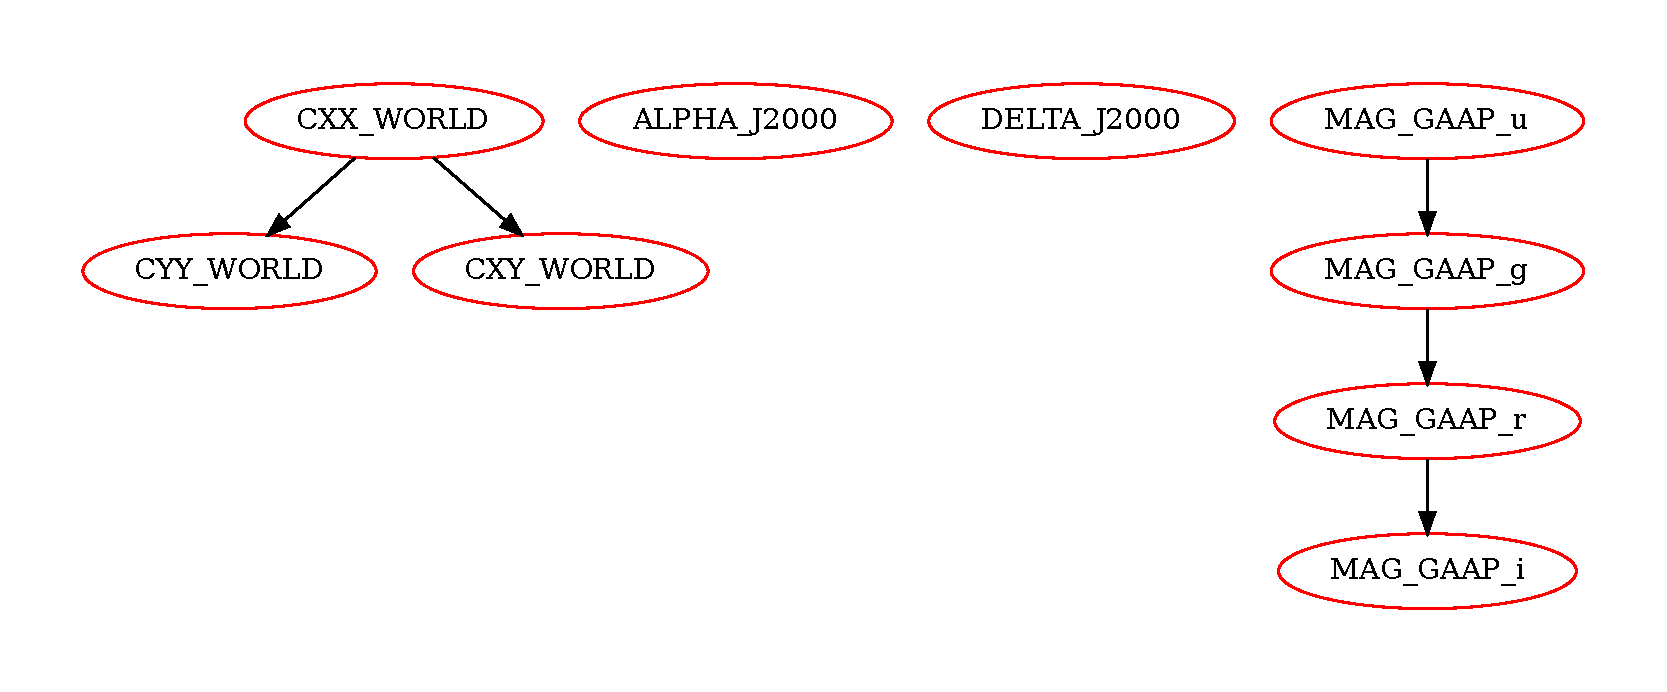
\includegraphics[width=\textwidth]{images/A2_prototypes/png_kids.pdf}
    \caption{\gls{KiDS}}
    \end{subfigure}
    \begin{subfigure}[]{0.5\textwidth}
    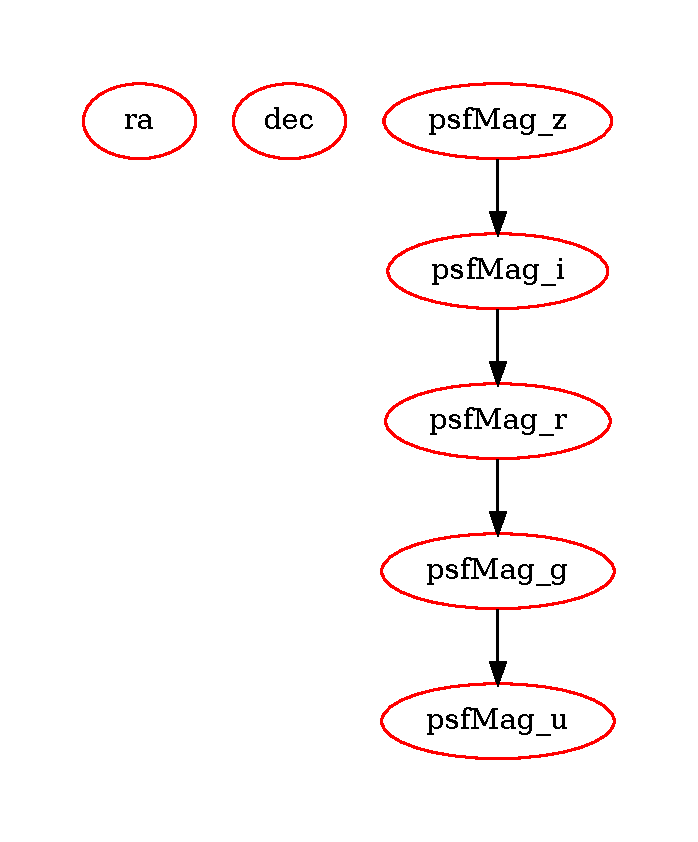
\includegraphics[width=\textwidth]{images/A2_prototypes/png_sdss.pdf}
    \caption{\gls{SDSS}}
    \end{subfigure}
    \caption{Two \glspl{PGN} trained over two different astronomical catalogs.}
    \label{fig:bayes1}
\end{figure}

\begin{figure}[htpb]
    \centering
    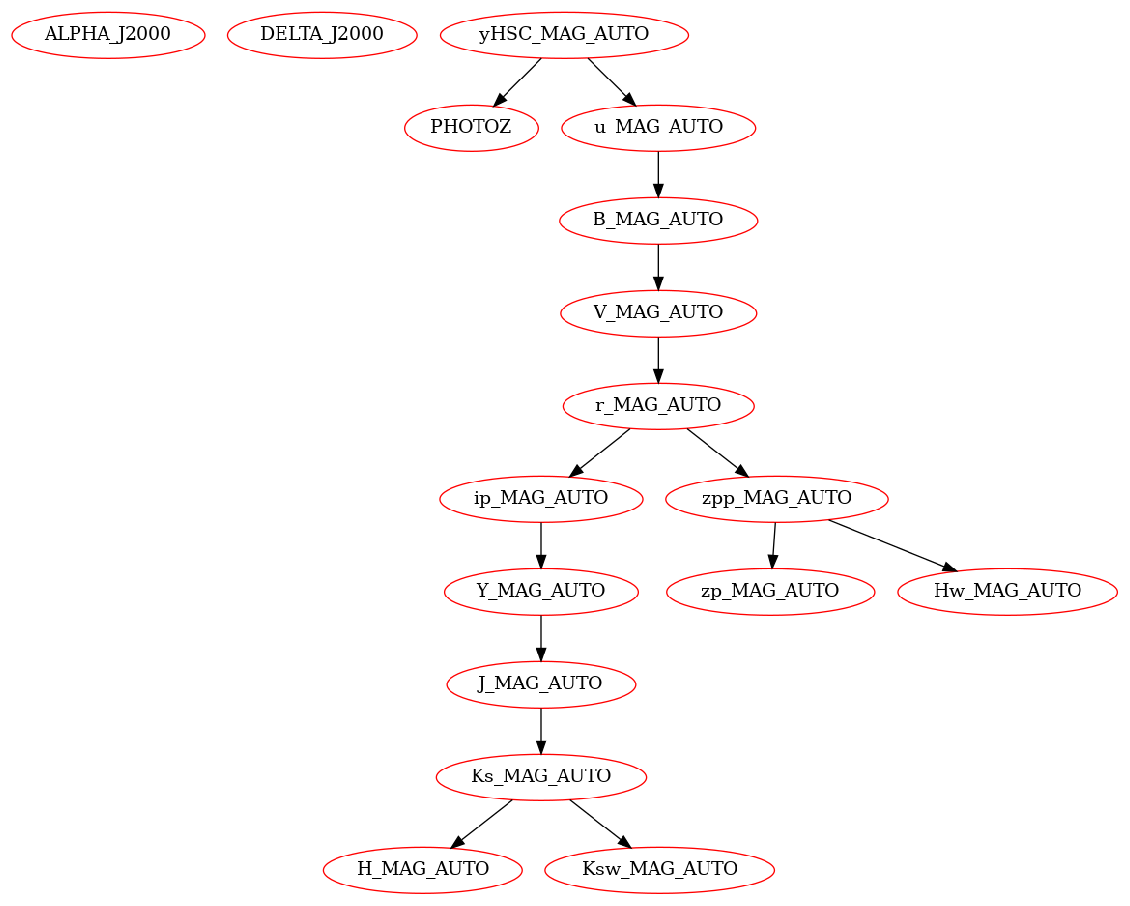
\includegraphics[width=\textwidth]{images/A2_prototypes/cosmos_bayes.png}
    \caption{\gls{PGN} trained over \gls{Cosmos}.}
    \label{fig:bayes2}
\end{figure}

\begin{table}[htpb]
    \begin{tabularx}{\textwidth}{c c c X c}
        \textbf{Bands} & \textbf{$\lambda$} &
        \textbf{\glsxtrshort{FWHM}} & \textbf{Filters} & \textbf{Description} \\ \hline
        \multicolumn{5}{c}{\textbf{Ultraviolet}} \\ \hline
        U & 365 nm & 66 nm  & u, u', u*             & \\
        \multicolumn{5}{c}{\textbf{Visible}} \\ \hline
        G & 464 nm & 128 nm & g'                    & Green \\
        R & 658 nm & 138 nm & r, r', R', Rc, Re, Rj & Red \\
        \multicolumn{5}{c}{\textbf{Near Infrared}} \\ \hline
        I & 806 nm  & 149 nm & i, i', Ic, Ie, Ij     & Infrared \\
        Z & 900 nm  &        & z, z'                 & \\
    \end{tabularx}
    \caption{\href{https://en.wikipedia.org/wiki/Photometric_system}{Subset of
            electromagnetic bands}. $\lambda$ corresponds to the wavelength.}
    \label{tab:bandas}
\end{table}


\printbibliography[segment=1]

\end{document}
